\chapter{Evaluation}
\label{chapter:validation}

\epigraph{``\textit{Let us change our traditional attitude to the construction
of programs: Instead of imagining that our main task is to instruct a computer
what to do, let us concentrate rather on explaining to human beings what we want
a computer to do.}''}{Donald E. Knuth}

 
This chapter describes the experimentation we conducted for
\correctingText{evaluating} the $\pi$SOD-M methodology. The chapter presents
three \correctingText{examples}. The first two \correctingText{examples} concern simplified
service-based applications that focus on the application's logic and explicit business rules. They show
how $\pi$SOD-M can be used for developing applications and exemplify the
consideration of non-functional aspects along the whole
development process. The last \correctingText{example}
(\textit{GesIMED}~\cite{valeriaThesis} application) \correctingText{aims to perform an
evaluation of our approach, analyzing the main differences and particularities
between SOD-M and $\pi$SOD-M.}

\newText{The objective of the experimentation was to evaluate the features and
concepts proposed by $\pi$SOD-M, considering the implementation of some
examples, and perform a comparison with SOD-M. This comparison focuses on
verifying which of those proposed aspects favored the development of
service-oriented applications in the presence of non-functional requirements. 
In this direction, our intention is: (i) analyze if it is possible to model
non-functional requirements from initial levels of abstraction in the
service-oriented development, (ii) and verify what are the advantages of using
the proposed approach, compared with the original proposal of SOD-M.}

% O objetivo principal deste capítulo é avaliar as características e conceitos
% adicionados em piSOD-M e fazer uma comparação com SOD-M, com a intenção de
% destacar que é possível modelar requisitos não funcionais desde níveis iniciais
% de abstração no desenvolvimento orientado a serviços. 


%  used for
% validating the specification and generation of the models proposed in
% $\pi$SOD-M. The validation split the thesis into parts, each one can be
% validated individually. This parts are: (i) the modelling of each $\pi$SOD-M
% model, (ii) the model transformations and (iii) the results.
% 
%  
% The validation is performed through three case studies. The first case study
% aims to perform a qualitative evaluation of our approach, analyzing the main
% differences and particularities between SOD and $\pi$SOD-M. The others case
% studies aim to validate and verify the use of $\pi$SOD-M and its
% environment, analyzing the positive results and the benefits to 
% model non-functional requirements from early stage of development.


%The thesis' validation of the  follows from the sub-validations.   
  
%\bigskip


% The \textit{IEEE Standard Computer Dictionary} \cite{ieeeDict} defines
% validation as \textit{the process of evaluating a system or component during or
% at the end of the development process to determine whether it satisfies specified
% requirements}. If we apply this definition to a methodology: \textit{Validation
% is the process of evaluating a method during or at the end of the development process to determine whether it
% satisfies specified requirements and eases the development of a system}. This
% chapter validates the methodology proposed in this thesis in order to verify
% whether it promotes a better development of reliable
% services composition applications. 

% The steps during the thesis were analyzed by application of laboratory case
% studies with an iterative and incremental approach. Thus, while the $\pi$SOD-M
% concepts have been defined, the concepts application have been made in each case
% studies to verify its validity. 

% The validation process has been performed in a continuous and
% progressive approach along the definition of $\pi$SOD-M. 


This chapter is organized as follows: section
\ref{sec:toPublishMusic_inpractice} shows the \textit{To Listen Music}
\correctingText{example}, section \ref{sec:crimes_inpractice} introduces the
\correctingText{example} \textit{Crime Map} and section \ref{sec:siw_gesimed}
introduces the \textit{GesIMED} \correctingText{example} that we used for
validating the methodology. Section \ref{sec:leassonsLearned} presents the lessons learned
with the validation process. Finally, Section \ref{sec:conclusion_validation} concludes
the chapter and discusses on validation results.


% From strategy for
% validation, the process was carried out with the development resolution step as
% part of an iterative process and feedback cyclic, allowing solve problems of
% concepts and its application while the methodology was being defined. Thus, in
% each step of methodology the validation was applied iteratively
% on two different case studies.
% 
% The process defined in the research method validation was therefore not
% a linear process, but iterative and incremental, thus providing the opportunity
% to go strengthen the results and learning from each research step.  
% 
% Following, each developed case study is described, indicating both the needs
% identified, and new contributions emerged from them, which are also shown
% graphically, using the methodology models. The case studies resolution were
% performed using the proposed approach. 



% \section{$\pi$SOD-M in Practice}
% \label{sec:execution}

% This section presents, in detail, the design and implementation of two case
% studies conducted to validate the method proposed in this
% thesis. Both case studies were developed using the models proposed by
% $\pi$SOD-M. 

% Following all models will be developed for this case and then
% describe the main aspects of the implementation of each of them.


\section{Example 1: To Publish Music}
\label{sec:toPublishMusic_inpractice}

 
An organization wants to provide the service-based
 application that monitors the music a person is listening during some periods
 of time and sends the song title to this person's Twitter or Facebook accounts.
 Thus, this social network user will have her status synchronized in Twitter or
 Facebook. The scenario begins by get through the music service Spotify for
 fetching the user's musical status. The social network services are then
 contacted to modify the user's status with the music information. The user can
 also download a specific music, he can proceed with the download process, which
 includes the payment process. 

The user can download a music, after having proceed with the
 payment via PayPal or credit card. All services are available via Spotify and
 this application needs to interact with Spotify users, so they can listen
 music, publish them on Facebook and Twitter, or buy music online. The scenario
 to monitor and publish songs has the User and Spotify actors.

The functionality of the application are: \textit{Search music;
Choose music; Download music; Listen Music; Buy music} and \textit{Publish music}. 

 \subsection{$\pi$-UseCase Model}
\label{sec:usecase_topublishMusic}

  
Figure \ref{fig:publishMusic_usecase} shows the main part of the use case model
for the \textit{To Publish Music} application\footnote{The complete
\textit{$\pi$-UseCase} model can be found in appendix \ref{append:diagrams}.}.
The $\pi$-UseCase model describes the system functions and constraints. Figures
\ref{fig:toolpublishMusic_usecase} and \ref{fig:toolpublishMusic_usecase2}
detail the model and configuration properties for the described example
(actual view taken from the $\pi$SOD-M environment).
Three restrictions are specified on the use cases described by the
model, two on the \textit{buy music} use case and a restriction on the
\textit{pay} use case. These restrictions are value and business constraints.
\textit{Buy music} restrictions are related to secure connection and to
ensure that the user needs to have an account in the music network. They are
marked using \textit{\#\ldots\#}, figures \ref{fig:publishMusic_usecase},
\ref{fig:toolpublishMusic_usecase} and \ref{fig:toolpublishMusic_usecase2}.
Notice that those NFRs and constraints will be the base to define assertions and
contracts by the transformations of models.



\begin{figure}[ht!]    
\centering
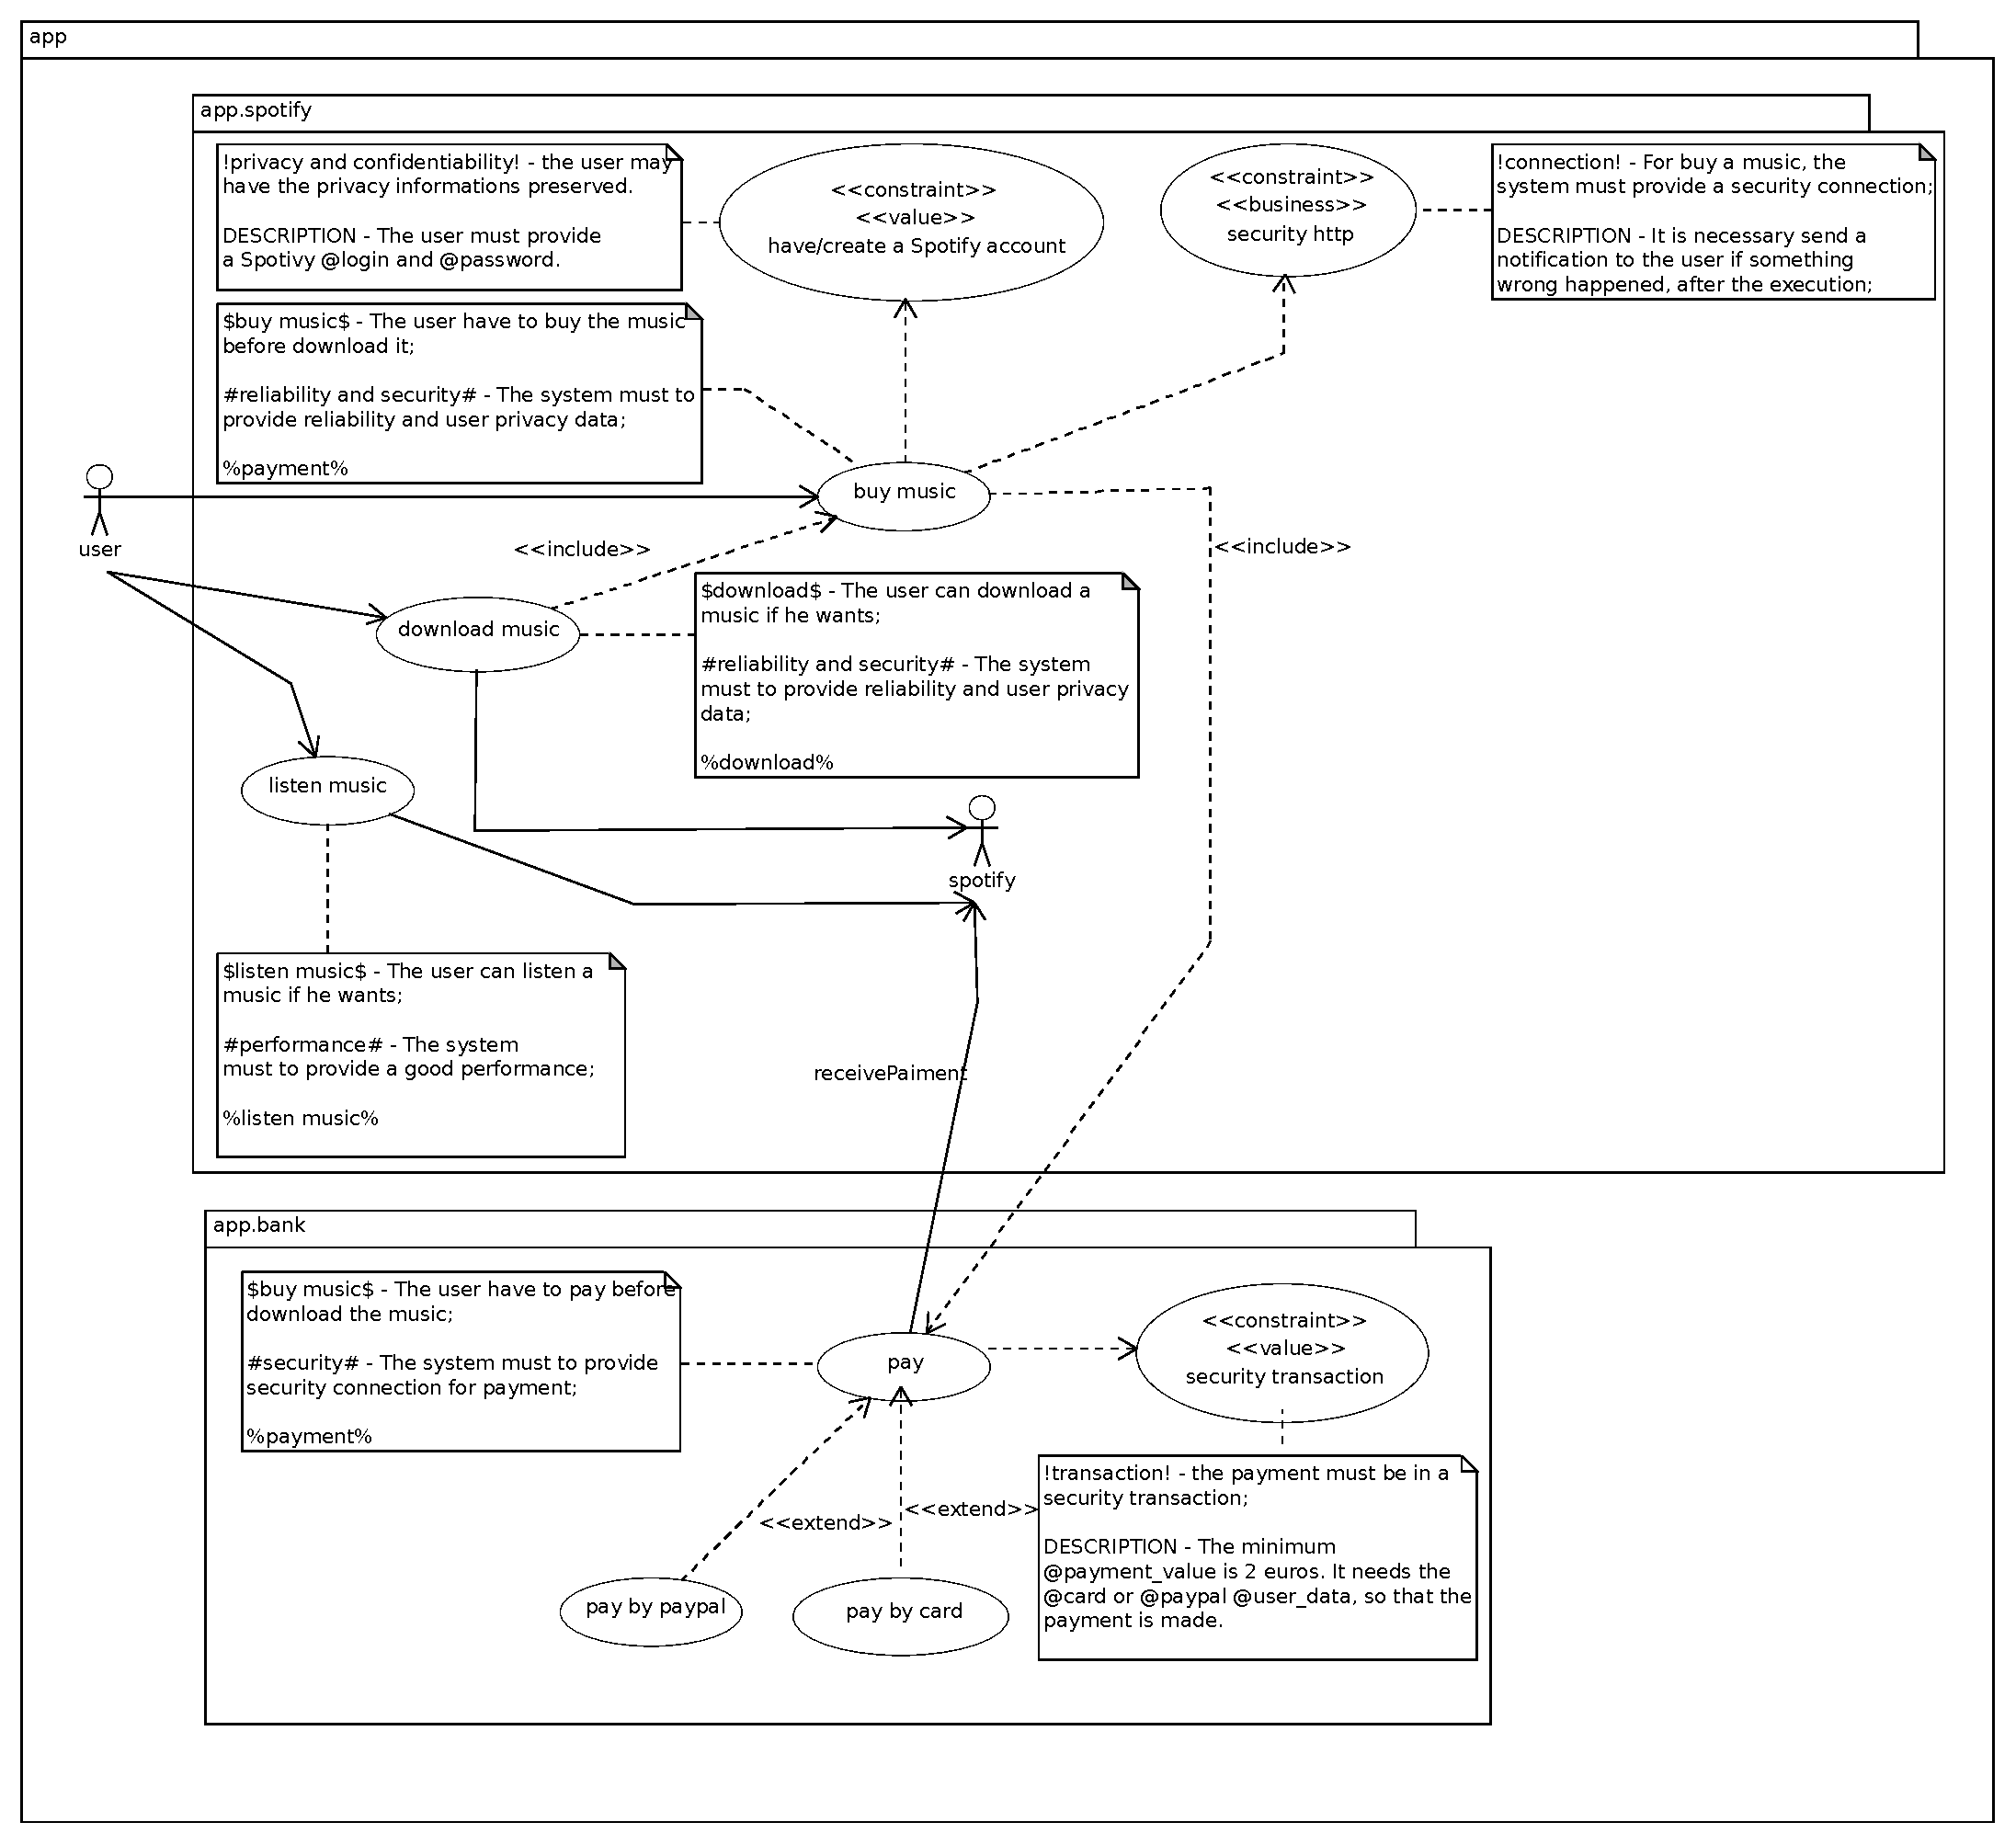
\includegraphics[width=.99\textwidth]{chapters/methodology/figs/piusecase/application/packages2.pdf}
\caption{\textit{To Publish Music} $\pi$-UseCase.}
\label{fig:publishMusic_usecase}
\end{figure} 


\begin{figure}[ht!]
\centering
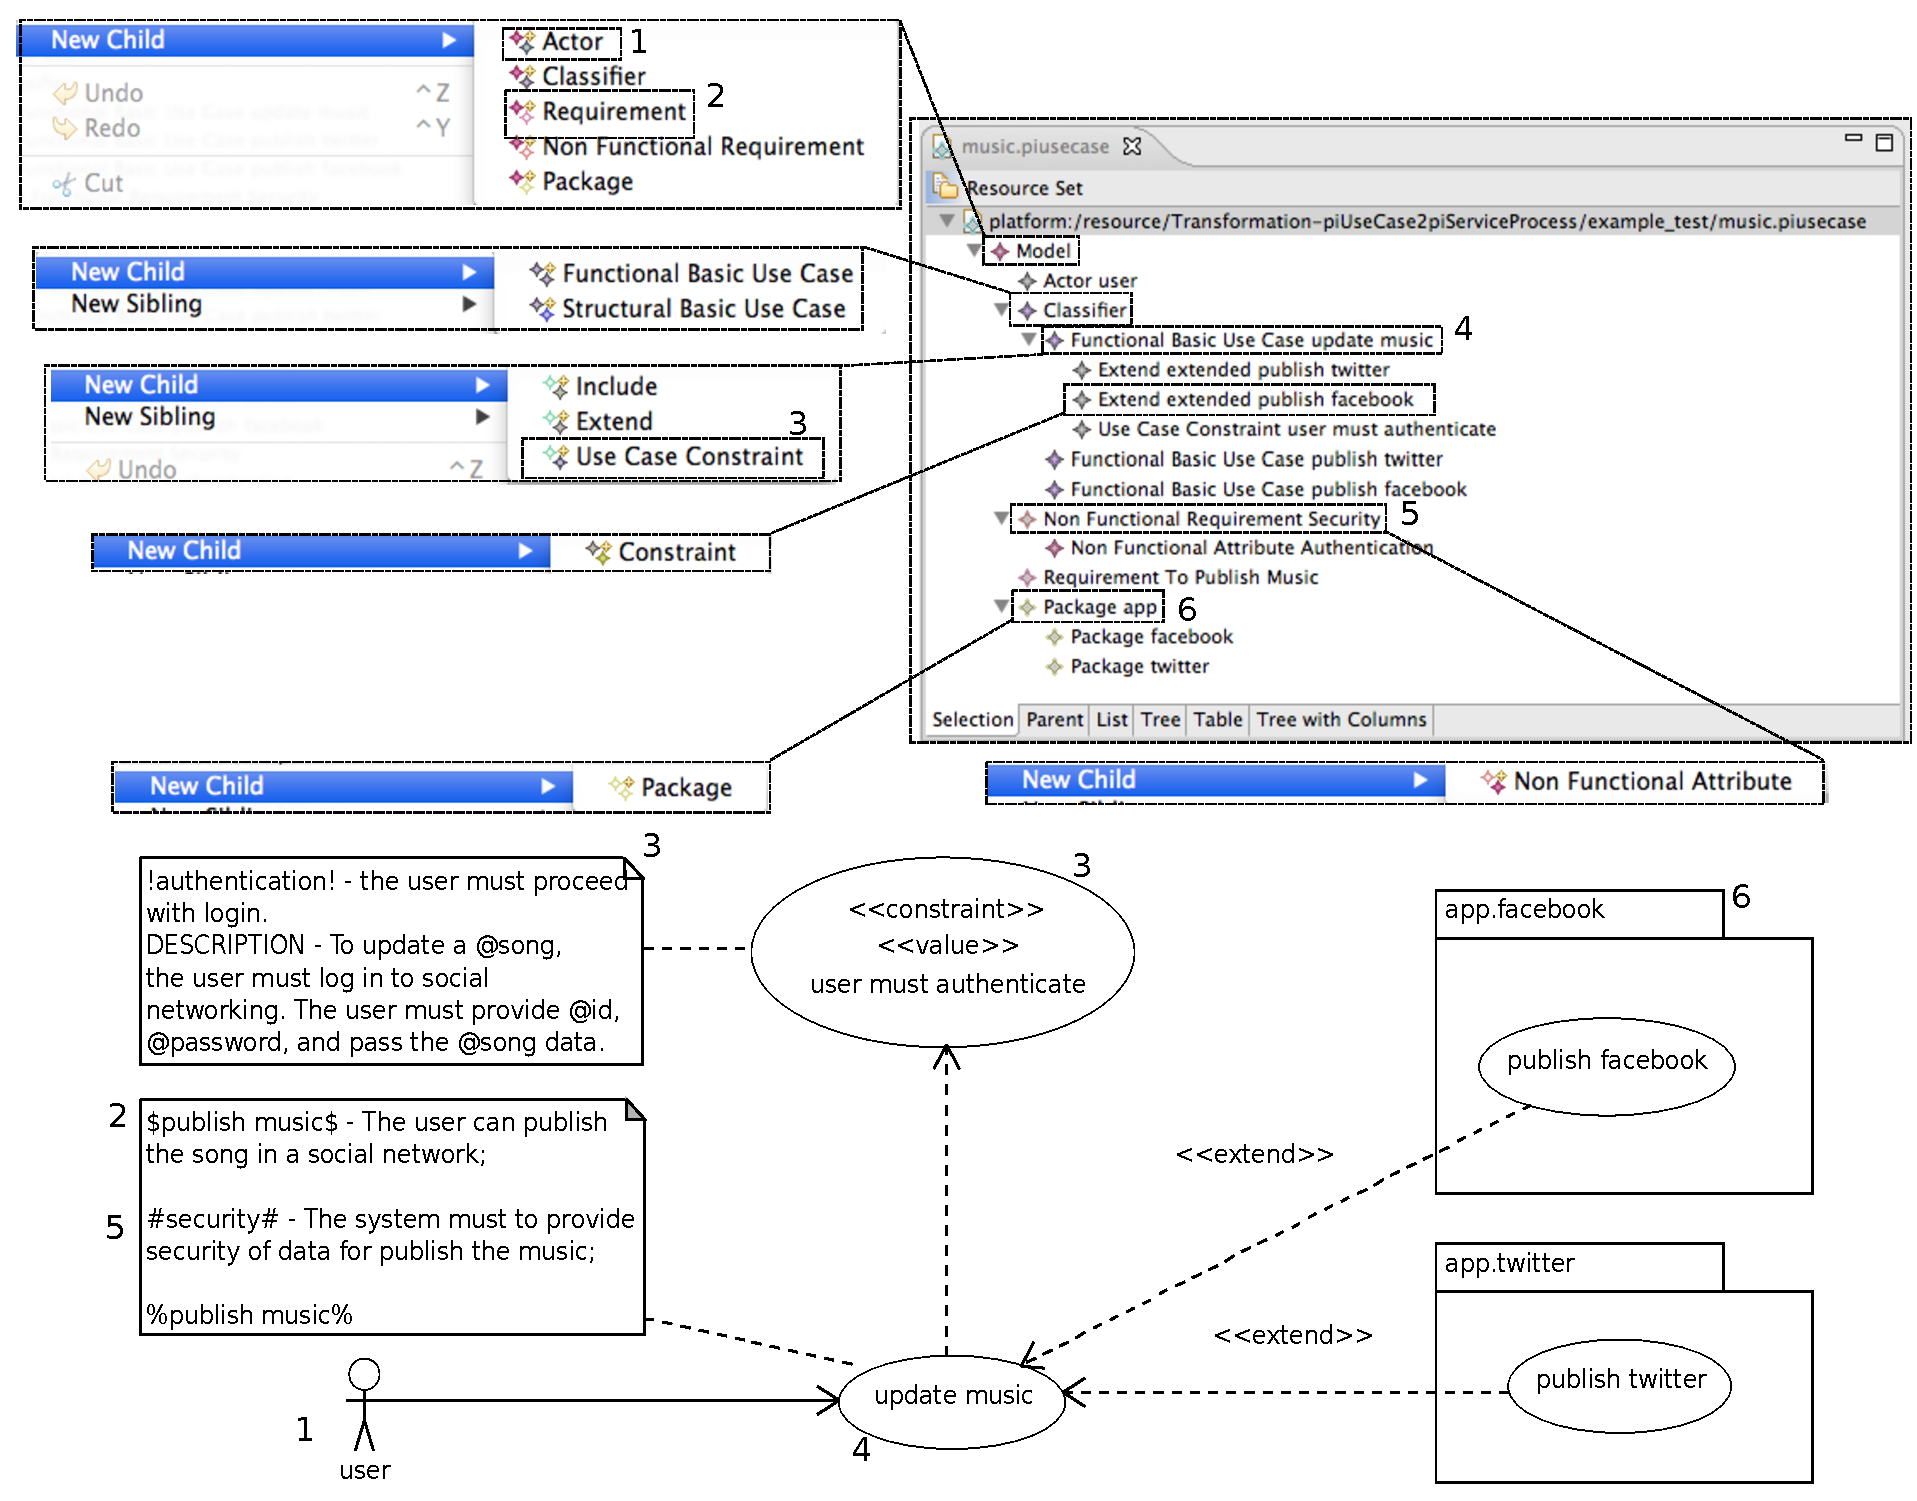
\includegraphics[width=.99\textwidth]{chapters/implementation/figs/create_model-UseCase.pdf}
\caption{\textit{To Publish Music} $\pi$-UseCase Environment Detail.}
\label{fig:toolpublishMusic_usecase}
\end{figure}

Figures \ref{fig:toolpublishMusic_usecase} and
\ref{fig:toolpublishMusic_usecase2} present the update music model and show how
the properties are defined in the $\pi$SOD-M environment. This example describes
the properties over the \textit{update music} (item 4, figure
\ref{fig:toolpublishMusic_usecase}) use case and the restriction over the
authentication process (item 3, figure \ref{fig:toolpublishMusic_usecase}). To
update a music in a social network, the user must be authenticated.

\begin{figure}[ht!]
\centering
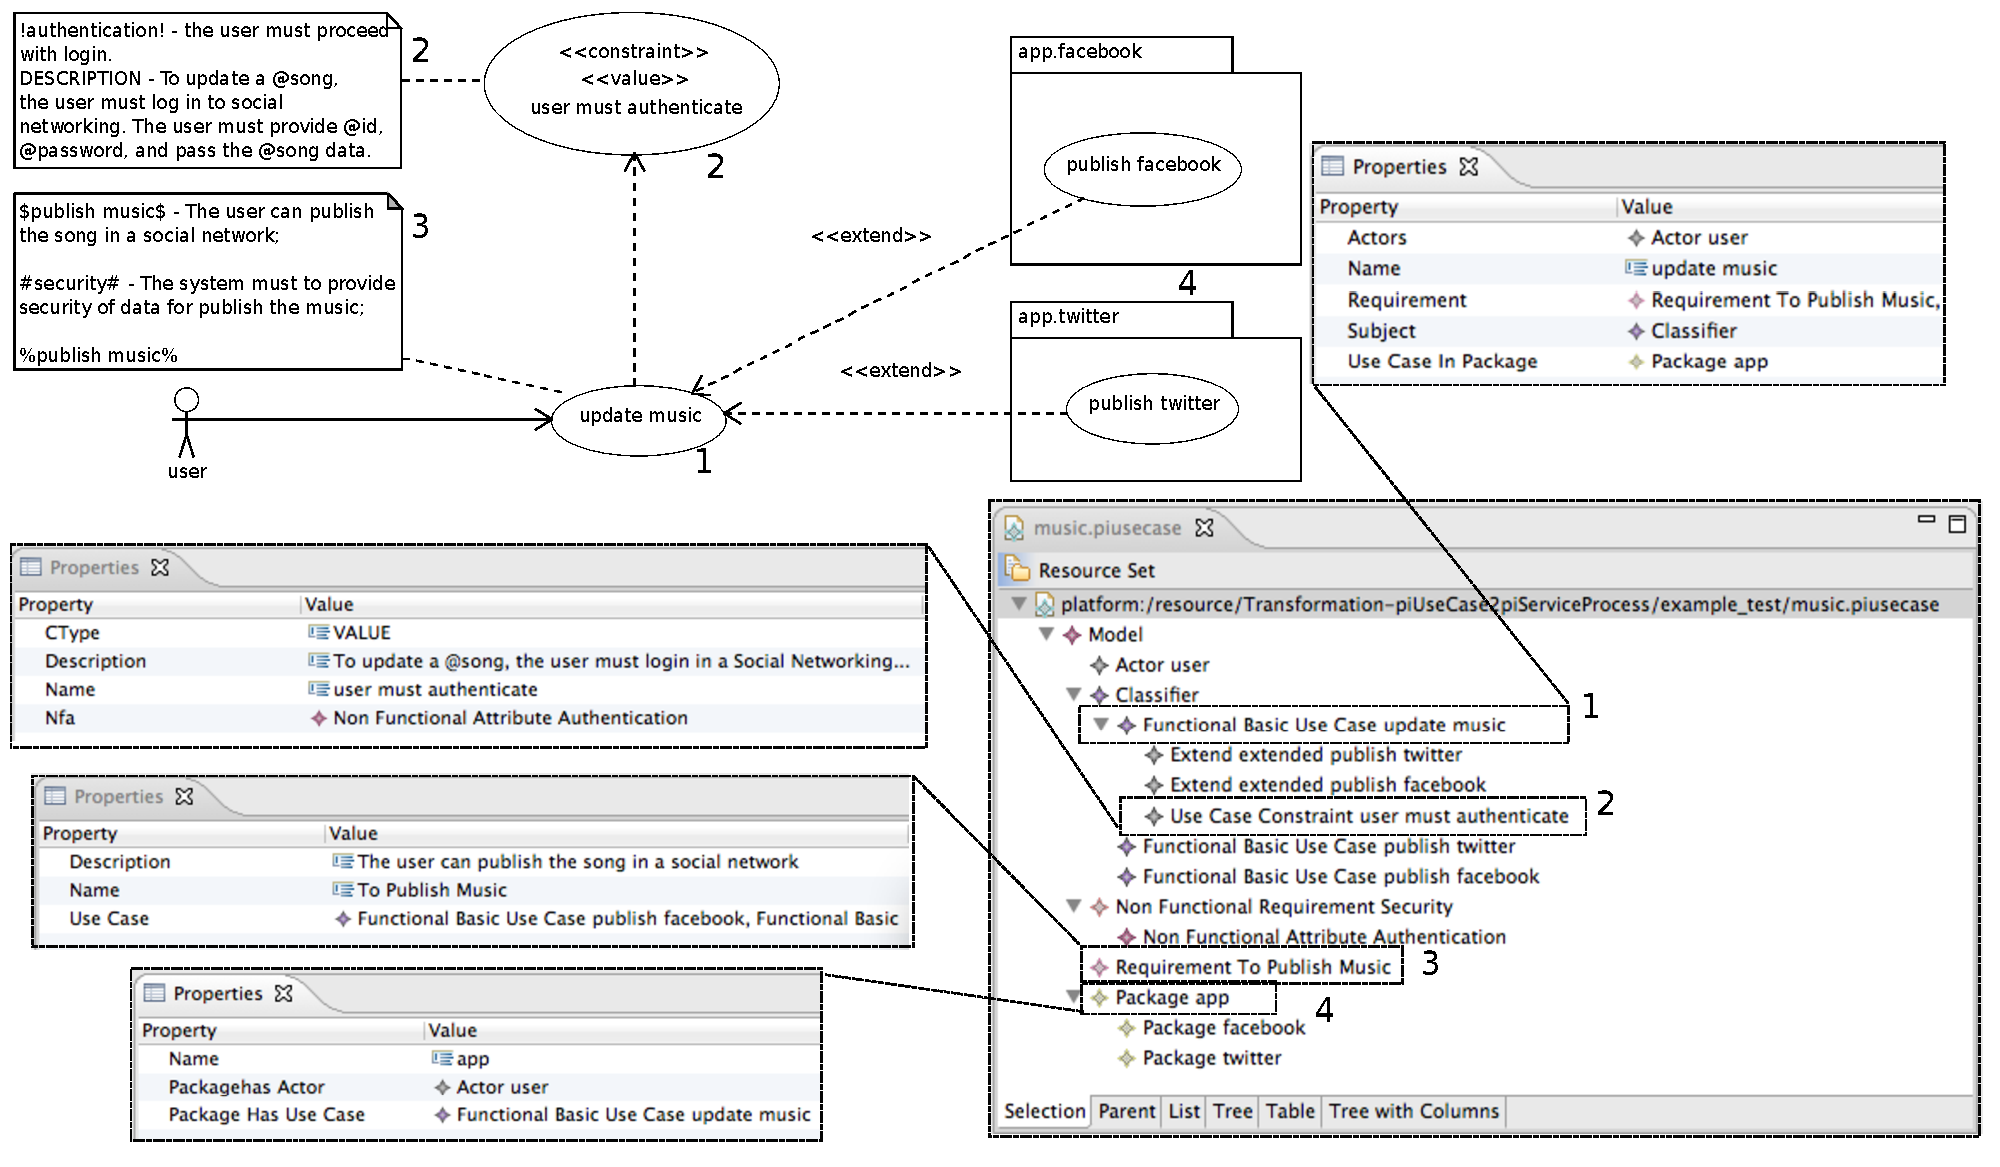
\includegraphics[width=.99\textwidth]{chapters/implementation/figs/model-UseCase.pdf}
\caption{\textit{To Publish Music}$\pi$-UseCase Environment Detail.}
\label{fig:toolpublishMusic_usecase2}
\end{figure}

The modeling of the application properties using the environment $\pi$SOD-M
are the same presented in the $\pi$-UseCase model, as described in Figure
\ref{fig:toolpublishMusic_usecase2}. For example, the authentication restriction
 details the type of constraint (\textit{VALUE}), a \textit{description},
 \textit{name} and a \textit{non-functional attribute}
 (\textit{authentication}). These properties are described in all constraints
 (item 2, figure \ref{fig:toolpublishMusic_usecase2}).

Figure \ref{fig:servicesToPublishMusic} shows the service components that must
interact with the \textit{application} and the interaction among them. There are
four services that are invoked to produce results for the \textit{Publish Music} application:
\textit{Spotify, Facebook, Twitter} and \textit{Bank}. 

\begin{figure}[ht!]   
\centering
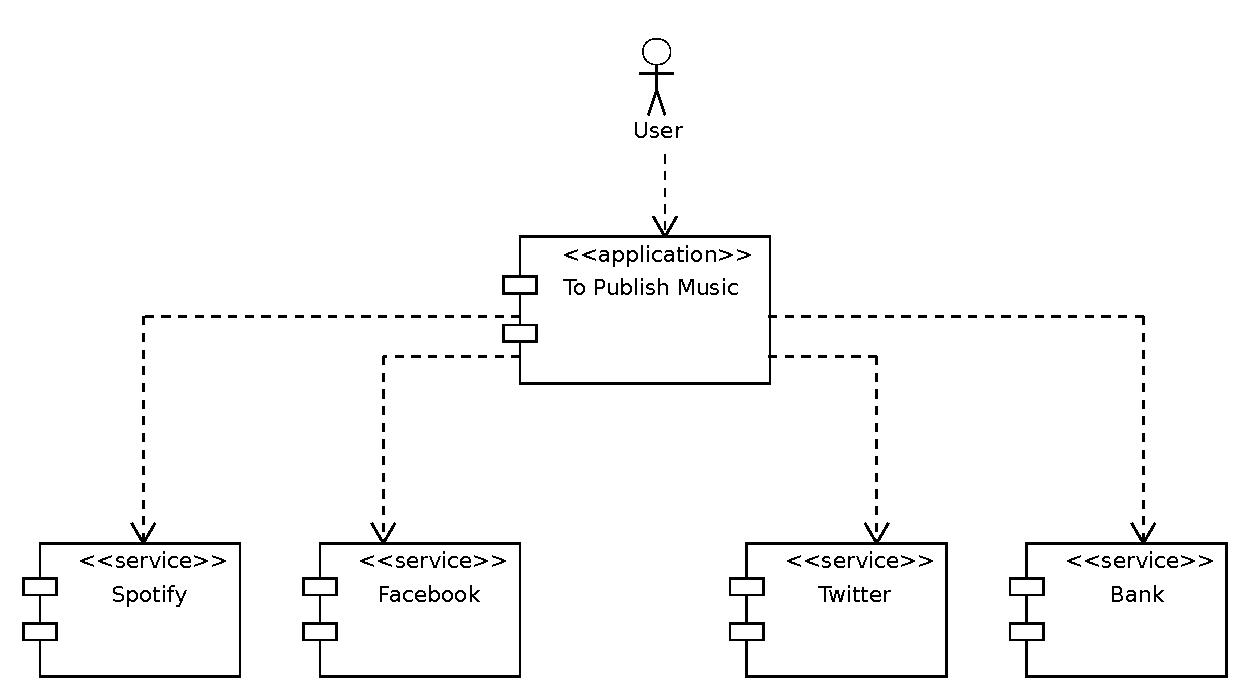
\includegraphics[width=0.8\textwidth]{chapters/validation/figs/toPublishMusic}
\caption{To Publish Music Services.}
\label{fig:servicesToPublishMusic}
\end{figure}  


 \subsection{$\pi$-ServiceProcess Model}
\label{sec:serviceProcess_topublishMusic}


Figure \ref{fig:publishmusic_piserviceProcessToolModelProperties} shows the
\textit{$\pi$-ServiceProcess} diagram for the execution of activities based on
contracts. We present here the part of the diagram produced from the concepts of the figure
\ref{fig:toolpublishMusic_usecase2}. The complete \textit{$\pi$-ServiceProcess}
diagram of the application is shown in figure \ref{fig:serviceprocessContract}.
Notice that it is necessary to represent each {\sc Constraint} modelled in a {\sc Contract} based service activity diagram. Each constraint
described in the previous model is transformed into a contract in the
$\pi$-ServiceProcess model.

\begin{figure}[ht!]
\centering
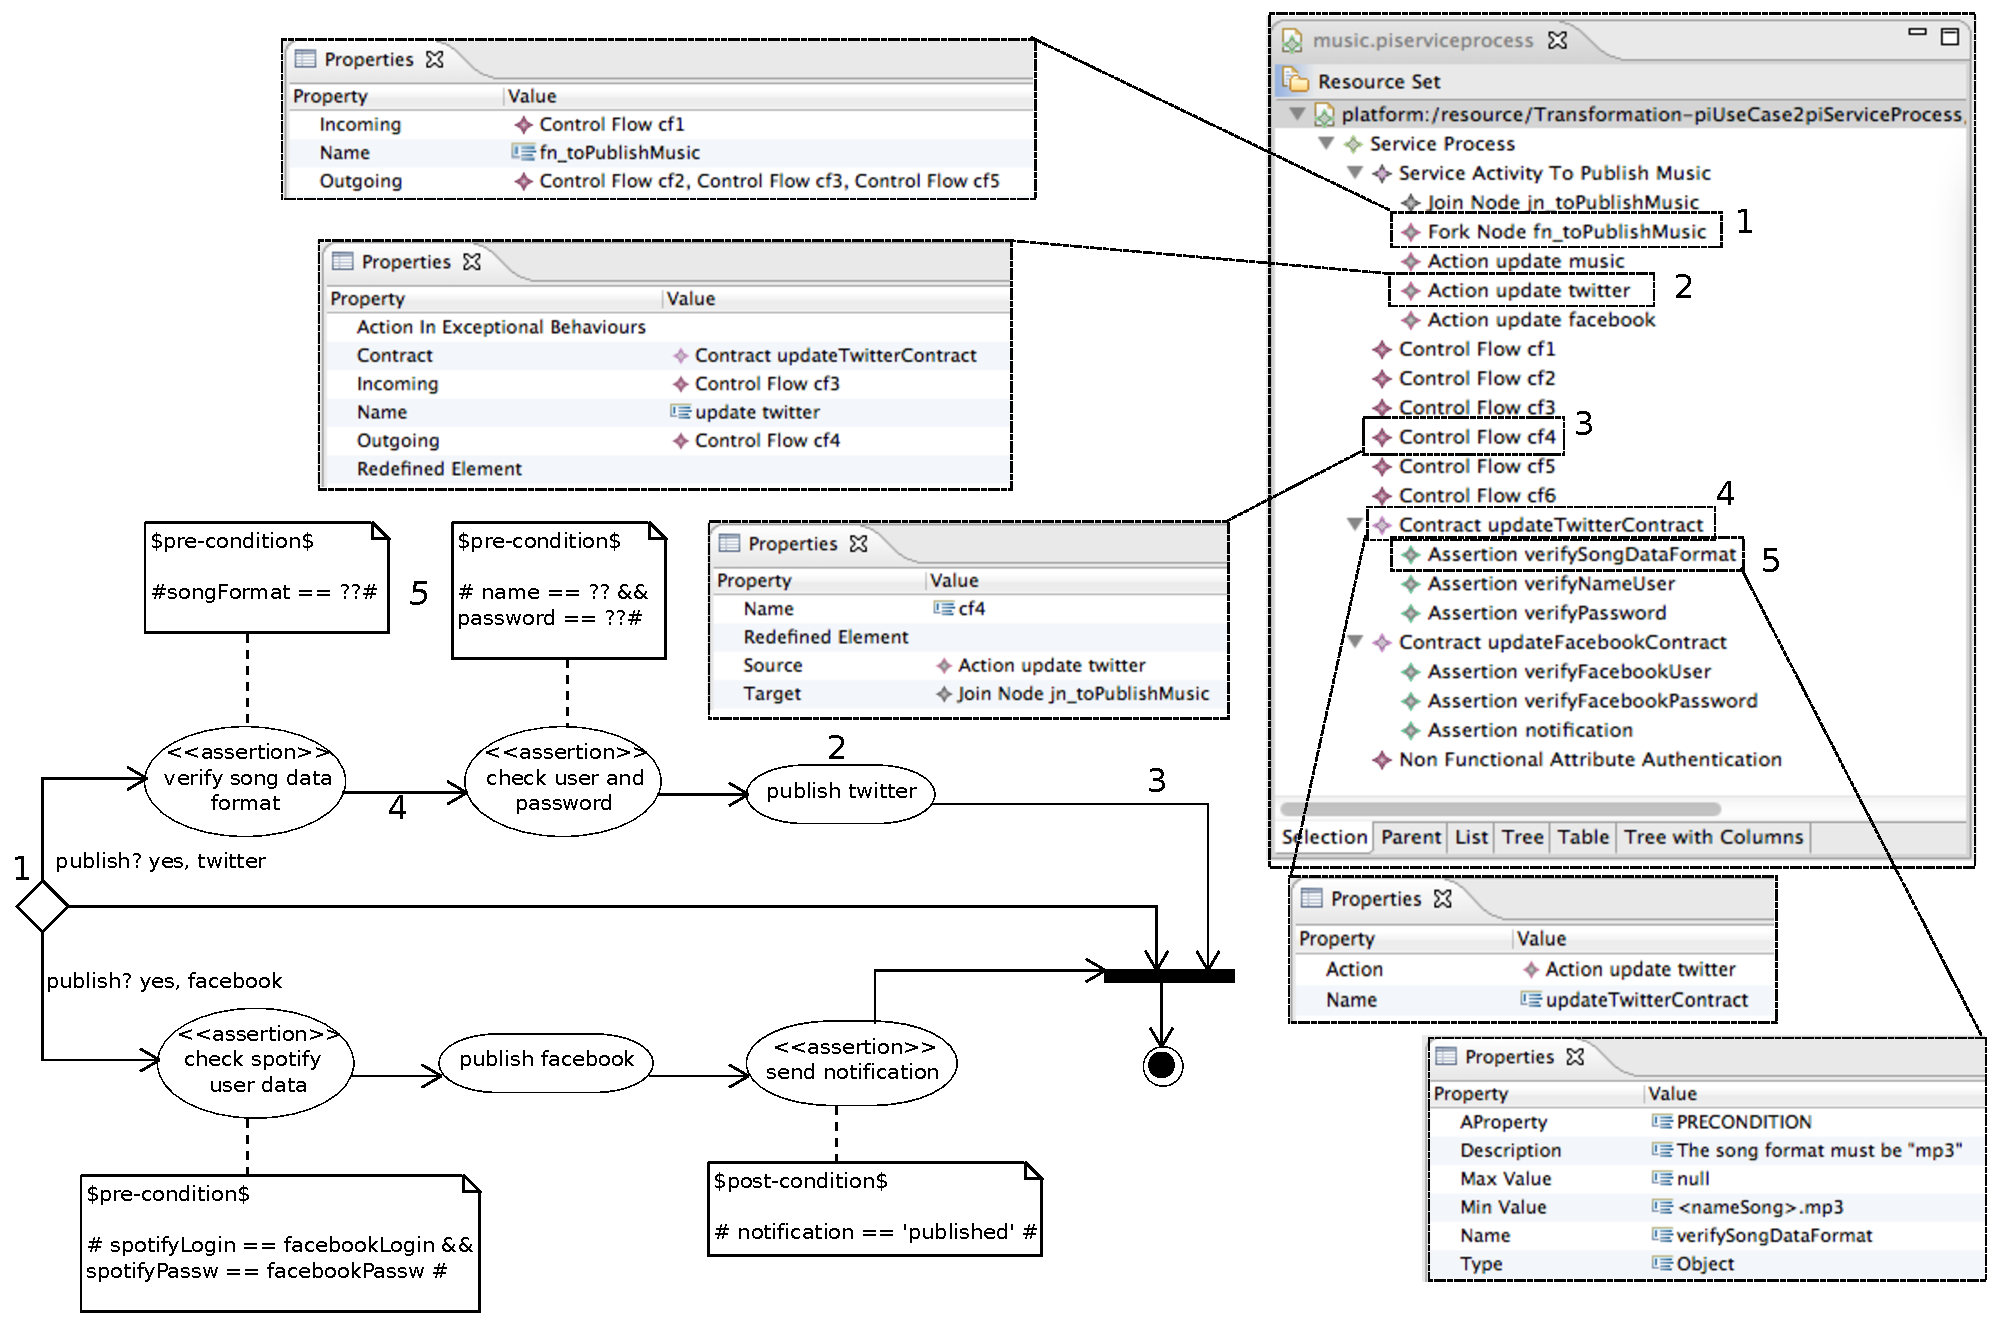
\includegraphics[width=.99\textwidth]{chapters/implementation/figs/model-ServiceProcess.pdf}
\caption{\textit{To Publish Music} $\pi$-ServiceProcess.}
\label{fig:publishmusic_piserviceProcessToolModelProperties}
\end{figure} 

\textit{Publish Twitter} and \textit{publish Facebook} (figure
\ref{fig:publishmusic_piserviceProcessToolModelProperties}) have pre- and
post-conditions assertions that are grouped into a contract for each service:
(i) verify if the user data are correct; (ii) if the user is already logged in
Spotify; As post-condition, it ensures the complete transaction and
verifies whether the payment authorization notification was sent to the user and to Spotify.
There may be different restrictions depending on the services participating in
the publish process. The user must be logged in Spotify in order to access
Facebook, and Facebook must send a ``successful login'' acknowledge which is
verified by the post-condition. For publishing a message, Twitter imposes
pre-conditions on the length of the message and user data login. In contrast,
Facebook only sends a confirmation acknowledge. Items 4 and 5 in figure
\ref{fig:publishmusic_piserviceProcessToolModelProperties} show the
pre-conditions for ``\textit{publish Twitter}'' concerning \textit{(i)} the format
of the music file and (\textit{ii}) access authorization credentials, namely
login and password.

\correctingText{The development of the $\pi$-ServiceProcess refine
the constraints into contracts for the services as shown
in Figure \ref{fig:publishmusic_piserviceProcessToolModelProperties}.}


% , about the payment authorization. To \textit{update} services, depending of each
% service, there may be different restrictions.

%  The Facebook service requires that the user is already logged on
%  Spotify and these data are the same as Facebook. As post-condition, it ensures
%  that the Facebook service send a notification of success. The Twitter service
%   requires pre-conditions over the message length and user privacy data, while
%   to update the Facebook is a necessary precondition and a confirmation notice
%   as post-condition. As a precondition for ``\textit{publish twitter}'' (itens
%   4 and 5, figure \ref{fig:publishmusic_piserviceProcessToolModelProperties}) it is necessary that
%   \textit{(i)} the music format is correct and (\textit{ii})  the twitter login and password is correct for the update.



 \subsection{$\pi$-ServiceComposition Model}
\label{sec:serviceComposition_topublishMusic}

 There are four external {\sc Business
Collaborators} in this application: \textit{Bank, Spotify, Twitter} and
\textit{Facebook} (items 3, figure
\ref{fig:topublishMusic_piserviceCompositionToolModel}). Figure \ref{fig:topublishMusic_piserviceCompositionToolModel} shows the application
services that consist of a set of functions: \textit{search music, select
music, buy music, download music, listen music} and \textit{publish music}. The
\textit{publish music} action calls two service collaborators (Facebook and
Twitter), and the \textit{buy music} action calls two functions of the Bank
service collaborator.
 
\begin{figure}[ht!]
\centering
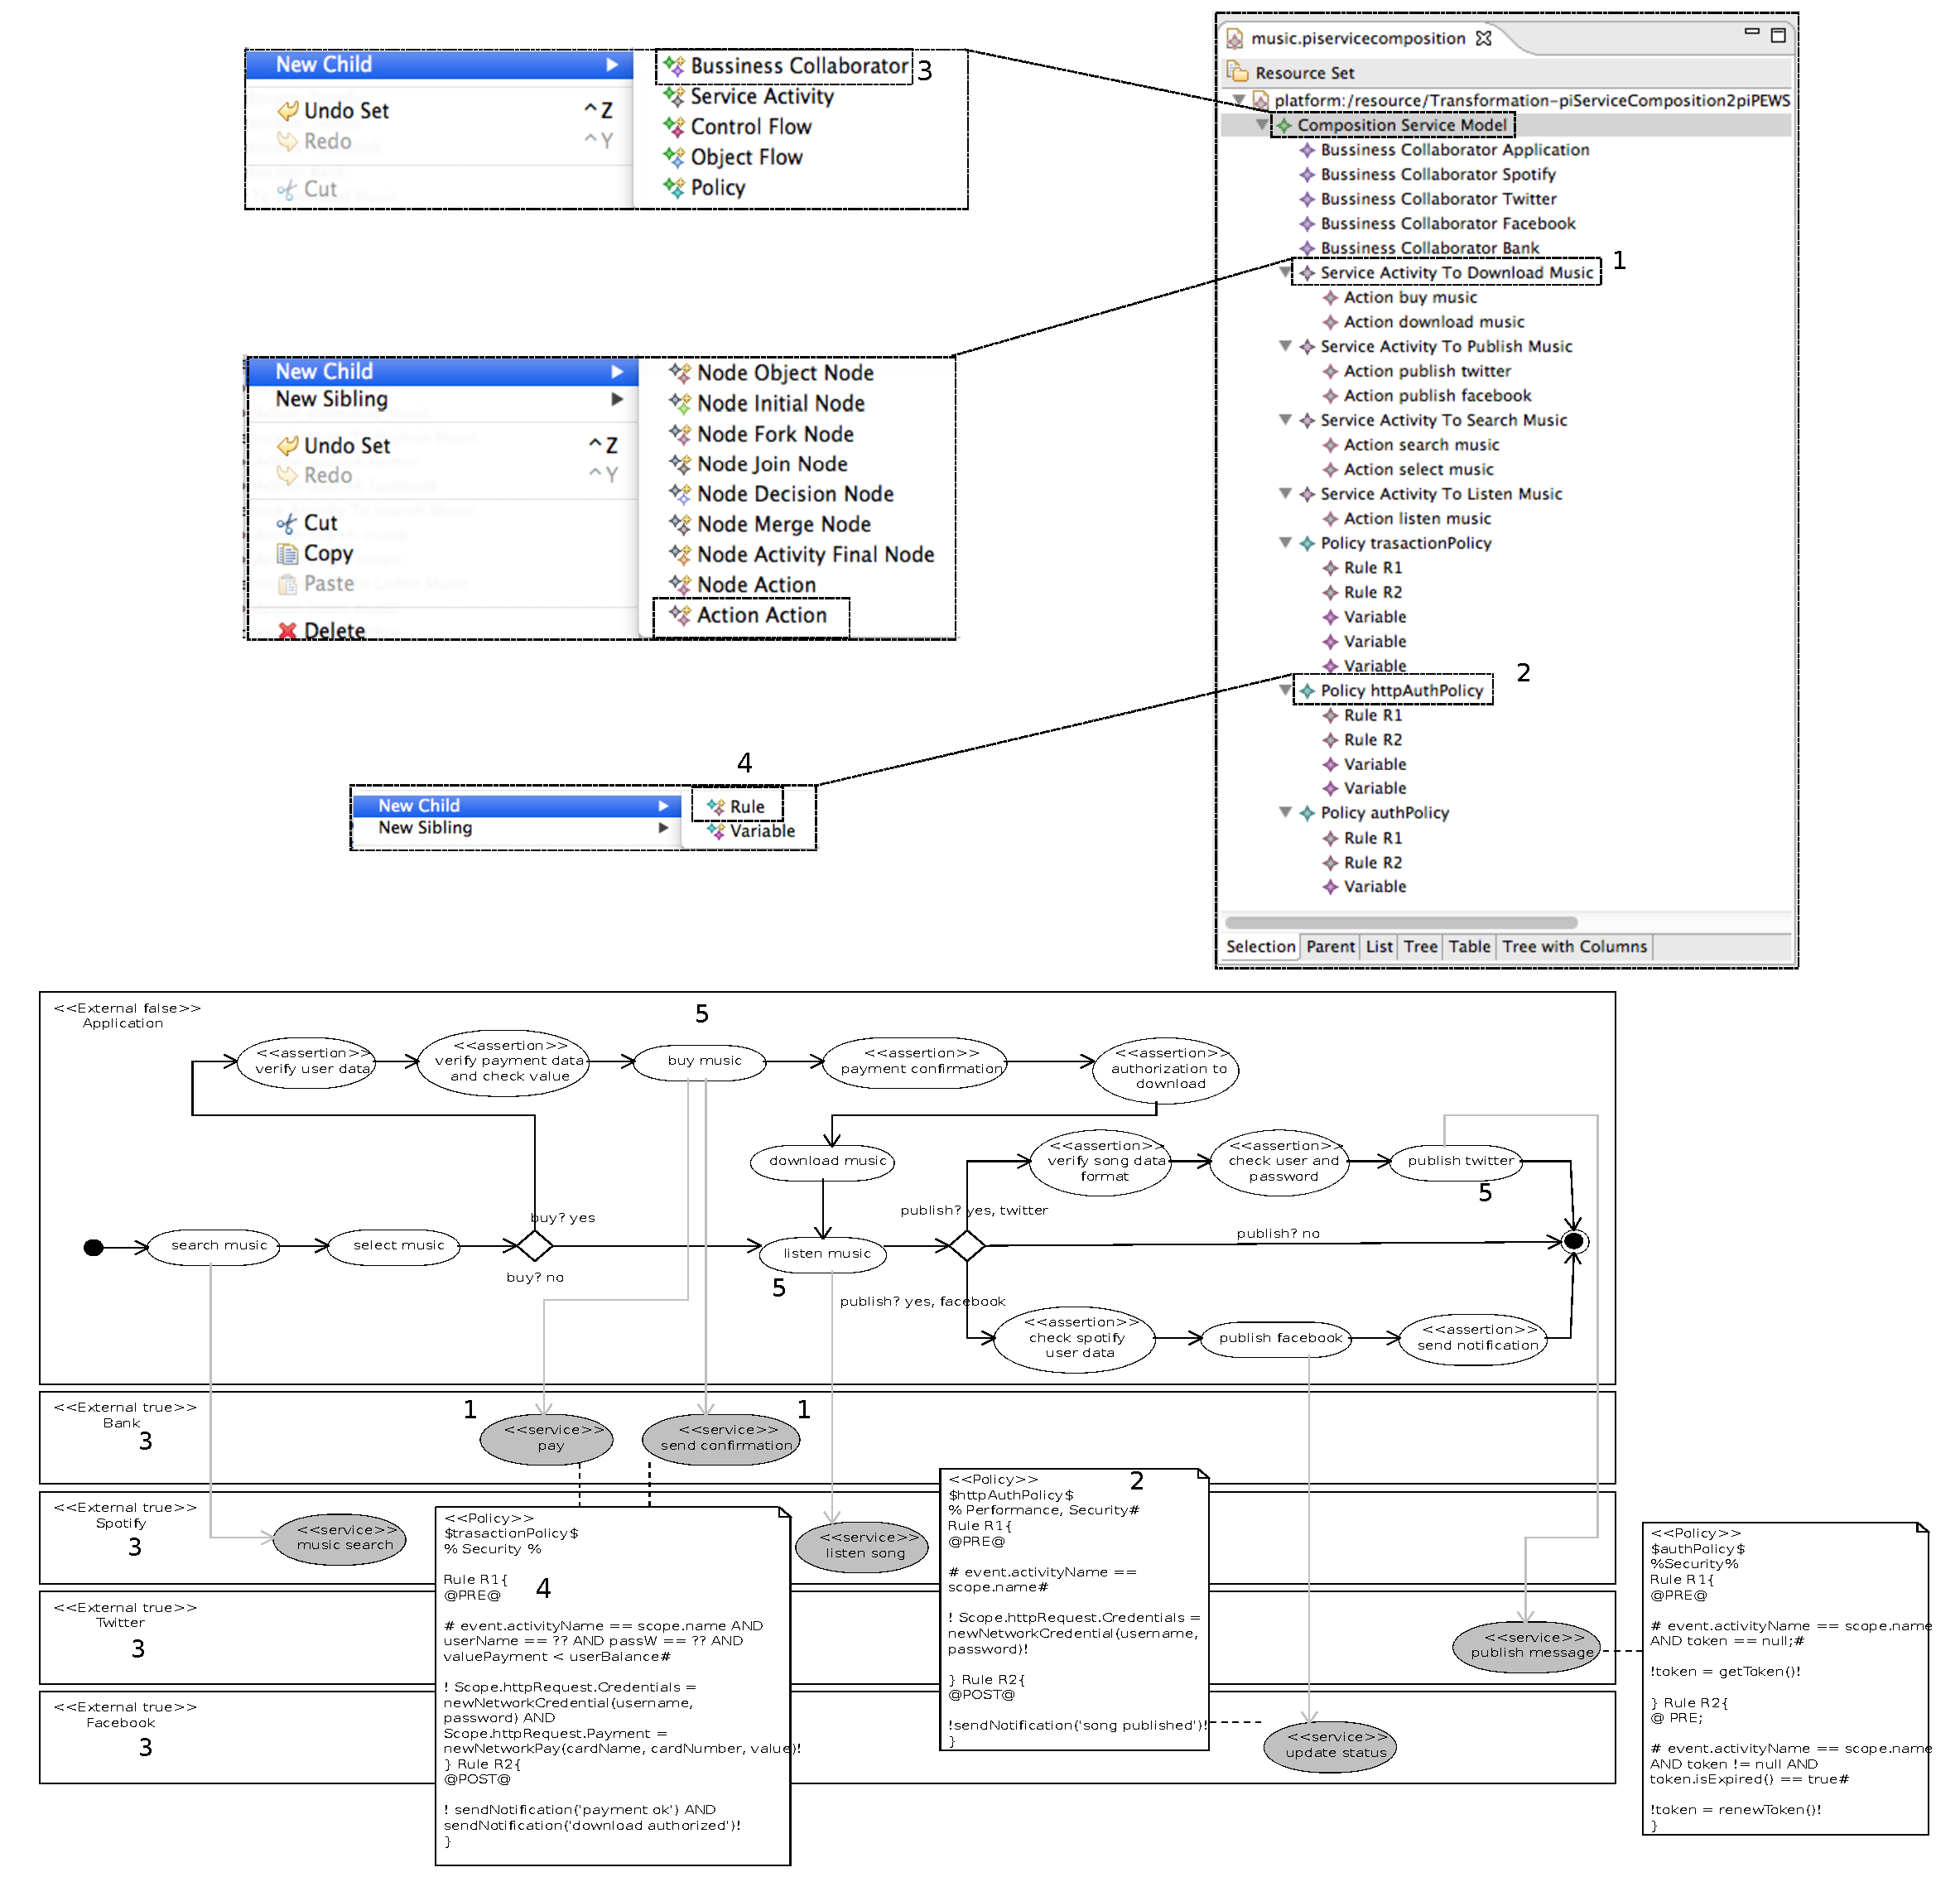
\includegraphics[width=.99\textwidth]{chapters/implementation/figs/create-model-Serviceconposition.pdf}
\caption{\textit{To Publish Music} $\pi$-ServiceComposition Model.}
\label{fig:topublishMusic_piserviceCompositionToolModel}
\end{figure}


The \textit{To Publish Music} $\pi$-ServiceComposition model defines three
policies: \textit{transactionPolicy} (item 4, figure
\ref{fig:topublishMusic_piserviceCompositionToolModel}), \textit{httpAuthPolicy}
(item 2) and \textit{authPolicy} (item 6). The \textit{trasactionPolicy}
verifies the Bank data restrictions over the payment and confirmation process.
The \textit{httpAuthPolicy} policy specifies rules over the
Facebook function for the authentication and notification processes. These rules
are executed during the publish massage function request. The
\textit{authPolicy} policy implements the open authentication protocol
required for accessing the Twitter service.


From the \textit{To Publish Music} rules and policies it is possible to model
and associate non-functional properties to services' compositions,
\textit{e.g.} the integration of information retrieved from different
social network services, automatic generation of an integrated view of the
operations executed in different social networks or for providing security in
the communication channel when the payment service is called.

From this stage, the \textit{$\pi$-PEWS} model (PSM) depicted in figures
\ref{fig:pewsRepresentation} and \ref{fig:contractRepresentation} can be
generated.

%  \subsubsection{$\pi$-PEWS Model}
% \label{sec:pews_topublishMusic}

 
% \begin{figure}[ht!]
% \centering
% 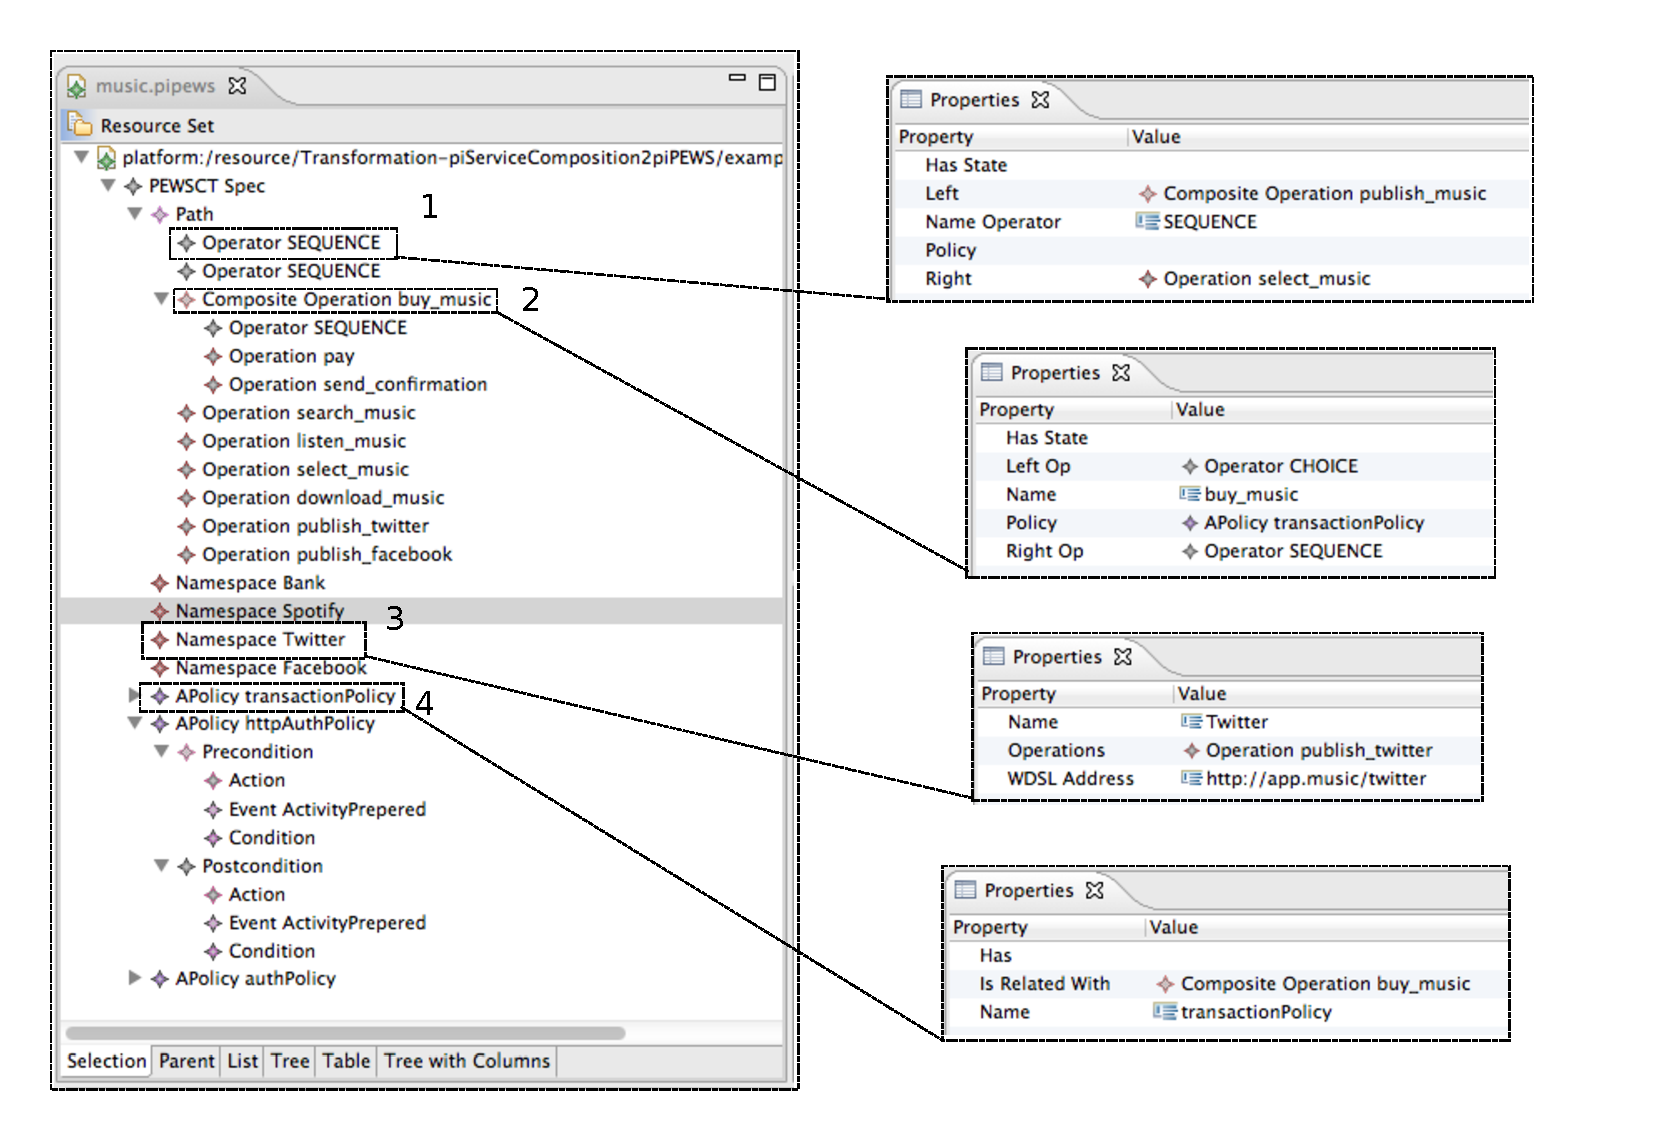
\includegraphics[width=.90\textwidth]{chapters/implementation/figs/create_model-PEWSProperties.pdf}
% \caption{$\pi$-PEWS Model Properties in $\pi$SOD-M Eclipse Plugin.} 
% \label{fig:piPEWSToolModelProperties}
% \end{figure}


% \section{Results}
% \label{sec:results} 
   

 
\section{Example 2: Crime Map}
\label{sec:crimes_inpractice}


The \textit{Crime Map} \correctingText{example} addresses the design and
implementation of a system that deals with statistical data on criminal activities. The system works
in conjunction with third-party services, in order to process a search supplied
by a user. The system must provide a public utility service to inform
citizens about the real crime situation in a particular location or region.
Making use of third party services, the application must provide a statistics crime portal. The result depends on user queries and upon a user
demand results can be presented on a map. The system also interacts with
micro-blogging, for looking up messages containing specific crime
information. The presentation of the data concerning criminal activities is
provided by the \textit{Police service}. The presentation of a locality map
crime is made by the \textit{Google Maps service} and messages presentation on
the micro-blogging is done by the \textit{Twitter service}. The system also has
a \textit{Post service}, for searching an address location that can be then
presented in a map by Google maps. The scenarios to query data and crime
statistics have the following actors: \textit{(i) User, (ii) Map service, (iii) Post service, (iv) Micro-blogging
service} and \textit{(v) Police service}, to query the criminal activities
(figure \ref{fig:usecaseCrimeMap_total}).

Considering the application functions, the crimes may be searched by types,
\textit{e.g.} \textit{theft, murder, kidnapping}, etc. The search can also be
made by city' district or region, for example, \textit{center, west, south,
north} or \textit{east}, and it can process search temporal criteria, for
example, crimes of the previous day of the last weeks or months. Finally, the
service can also process conjunctive queries, \textit{e.g.}, \textit{the number of kidnapping of a specific district in the last month}.

Whenever a new crime is published by the police, the system should post a
 message on Twitter stating the new crime, with a specific hashtag,
 \textit{e.g.} \textit{\#crime043\_kidnapping\_center\_05-08-2012}. The hashtag
 structure contains the crime number, type, local and the day it happens. From
 this, users can comment about the crime and these comment will appear in the
 application interface. All users must have an account to use the application.

 The application functionalities are: \textit{Choose search type of crime; see
 crime information; Receive information on the chosen query; See map; List crimes;}
 and \textit{Comment about a crime.}
 
 Non-functional requirements for this application include: \textit{queries
 response performance, crime information validation}, \textit{crime
 information presented in a map} and \textit{ensuring crimes data security.}

\subsection{$\pi$-UseCase Model}
\label{sec:usecase_crimesMap}


% The modeling of the system starts with the $\pi$-UseCase model. This involves
% determining the services identified in the list of requirements, which final
% consumers identified in the list of business services, and which of the will be
% end consumers or service users. Thus, it is possible to identify the modeling
% elements that are part of the use case model.
 
 Figure \ref{fig:usecaseCrimeMap_total} presents the Crime Map $\pi$-UseCase
model. This model includes examples of \textit{business, value}
and \textit{exceptional behaviours} constraints. The application accesses
data from third party services to provide the user an easy way to visualize new
information, these services are: \textit{Map, Police, Postal} and
\textit{Microb-logging Services}. 

The user interacts with the application that will perform the services
for obtain and publish details about the crimes. The services are modeled as
actors (they are external applications). Each service has a set of functions
that can be performed. The $\pi$-UseCase model describes both the external services
and the functionality of the application (see figure
\ref{fig:usecaseCrimeMap_total}).

\begin{figure}[ht!]   
\centering
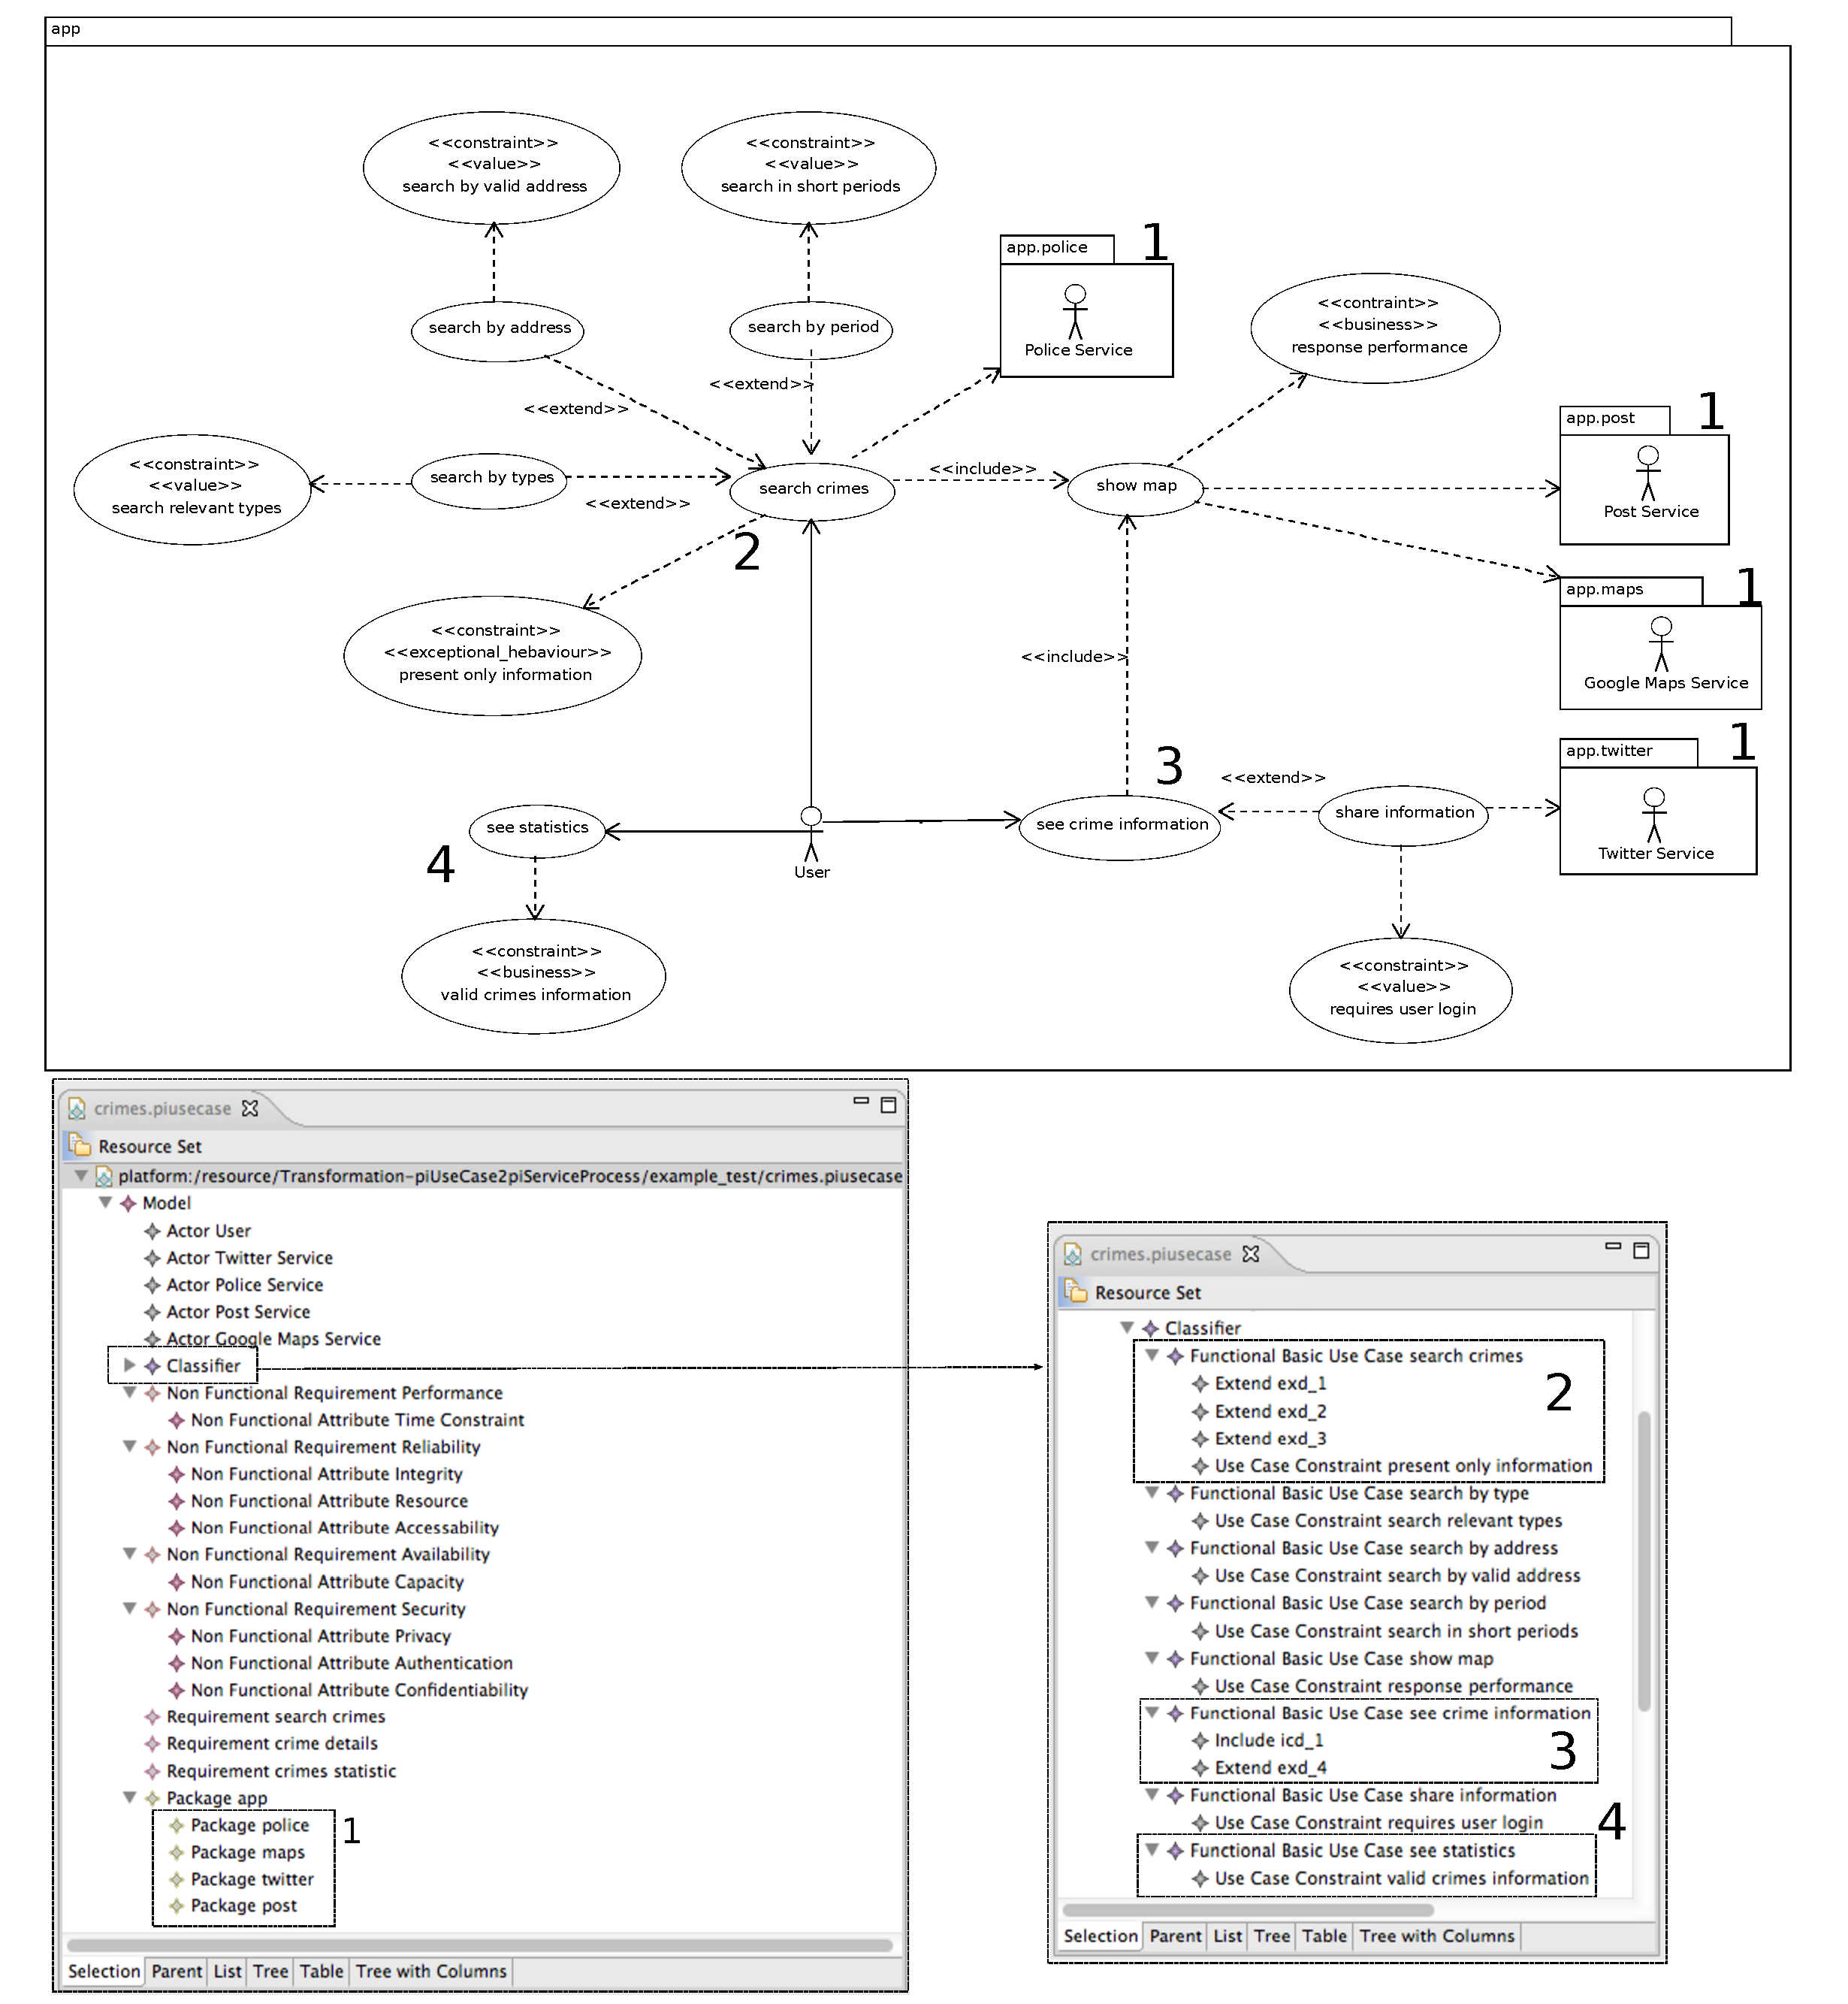
\includegraphics[width=0.99\textwidth]{chapters/validation/figs/crimes_useCase}
\caption{Crime Map $\pi$-UseCase.}
\label{fig:usecaseCrimeMap_total}
\end{figure}  

The user can search for crimes and view its occurrences in a map. The search may be performed by \textit{type of
crime, region} or \textit{period}. The user can also perform a search that
combines these criteria. If the application's user does not choose any
option, the search will retrieve up to 30 recent occurrences. If the location
maps service is unavailable or there is no response from it after 5 seconds,
only the crimes information will be presented, without a map view.


Figure \ref{fig:usecaseCrimeMap_total} also
presents the $\pi$-UseCase model tree representation generated by the $\pi$SOD-M
environment model .Figures \ref{fig:usecaseCrimeMap1} and \ref{fig:usecaseCrimeMap2} detail the
use cases and constraints presented in Figure
\ref{fig:usecaseCrimeMap_total}. 

\begin{figure}[ht!]   
\centering
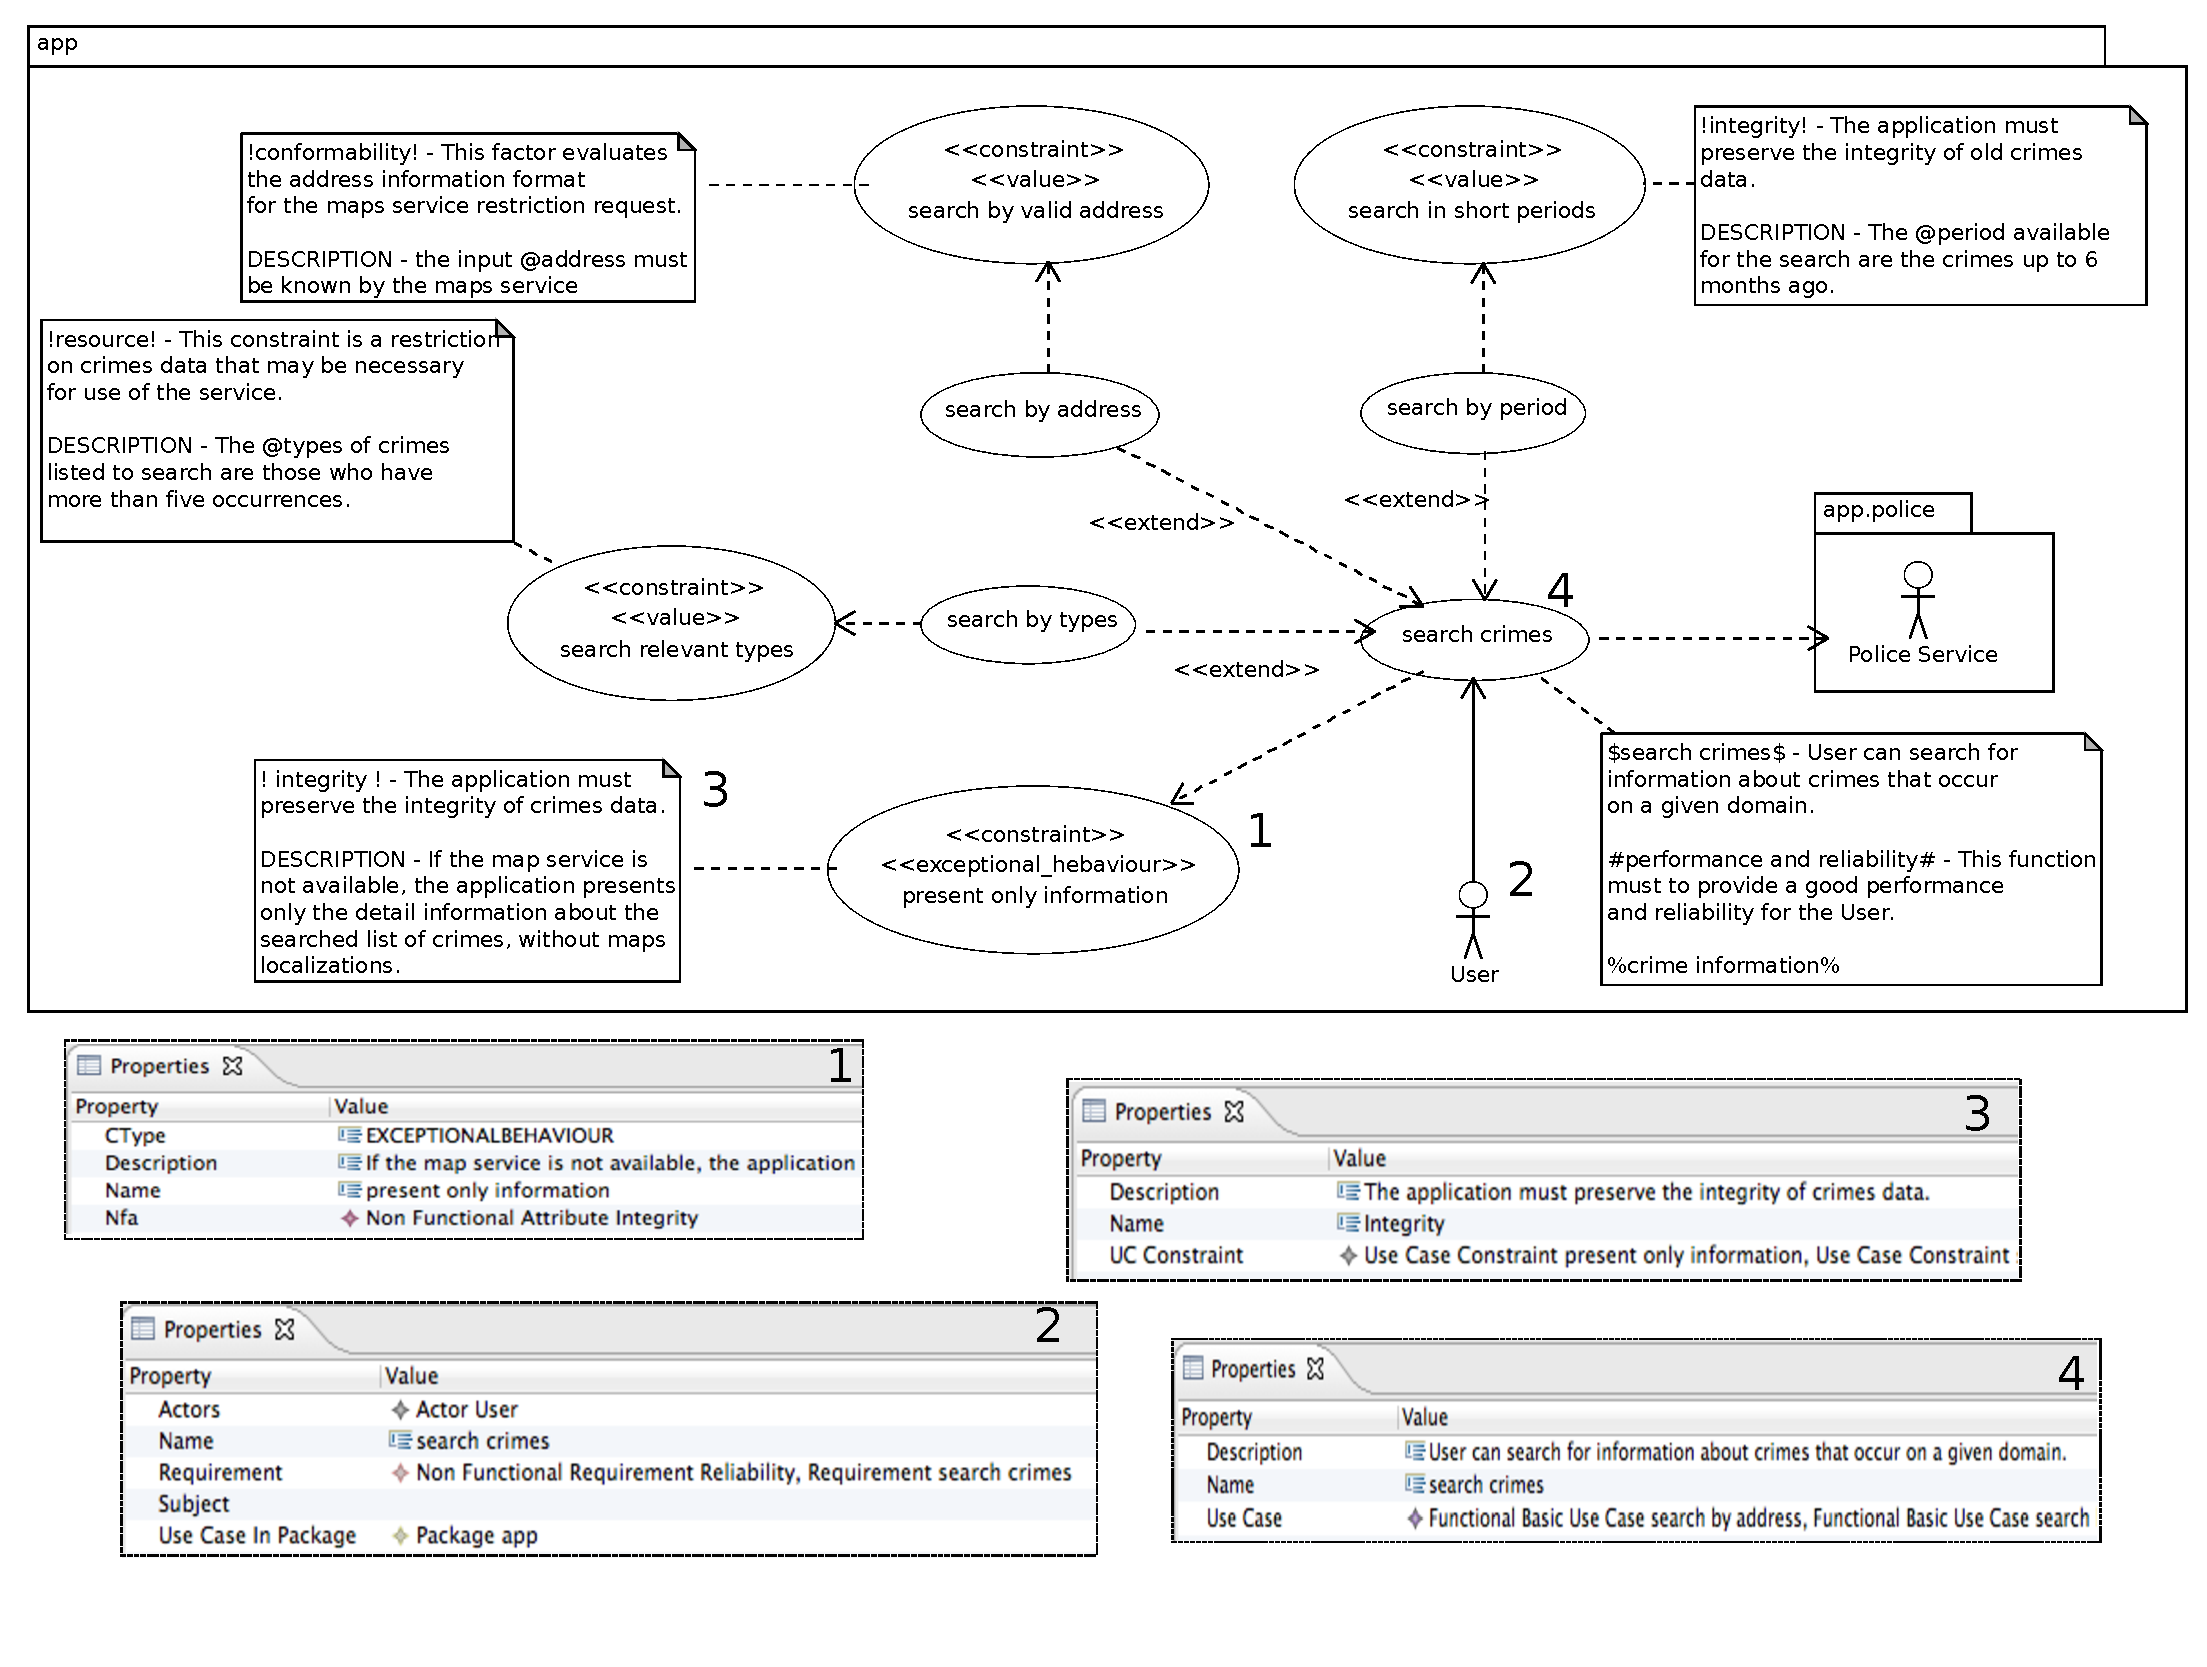
\includegraphics[width=0.99\textwidth]{chapters/validation/figs/crimes_useCase1}
\caption{\textit{Search crime} $\pi$-UseCase Detail.}
\label{fig:usecaseCrimeMap1}
\end{figure}  

The \textit{search crimes} use case (Figure \ref{fig:usecaseCrimeMap1})
requests the \textit{Police} service to verify the crimes according to the
parameters supplied by the user. The restriction of this use case depends on
the parameters selected by the user. If the user chooses one or several types of
specific crime's type, the system will present those crimes that have more than
five occurrences. For \textit{search by address}, the address must comply with
the restrictions of the police service, the research can be done by street,
neighborhood, city or district. \textit{Search by period} will provide only
occurrences within the last six months.
 
\begin{figure}[ht!]   
\centering
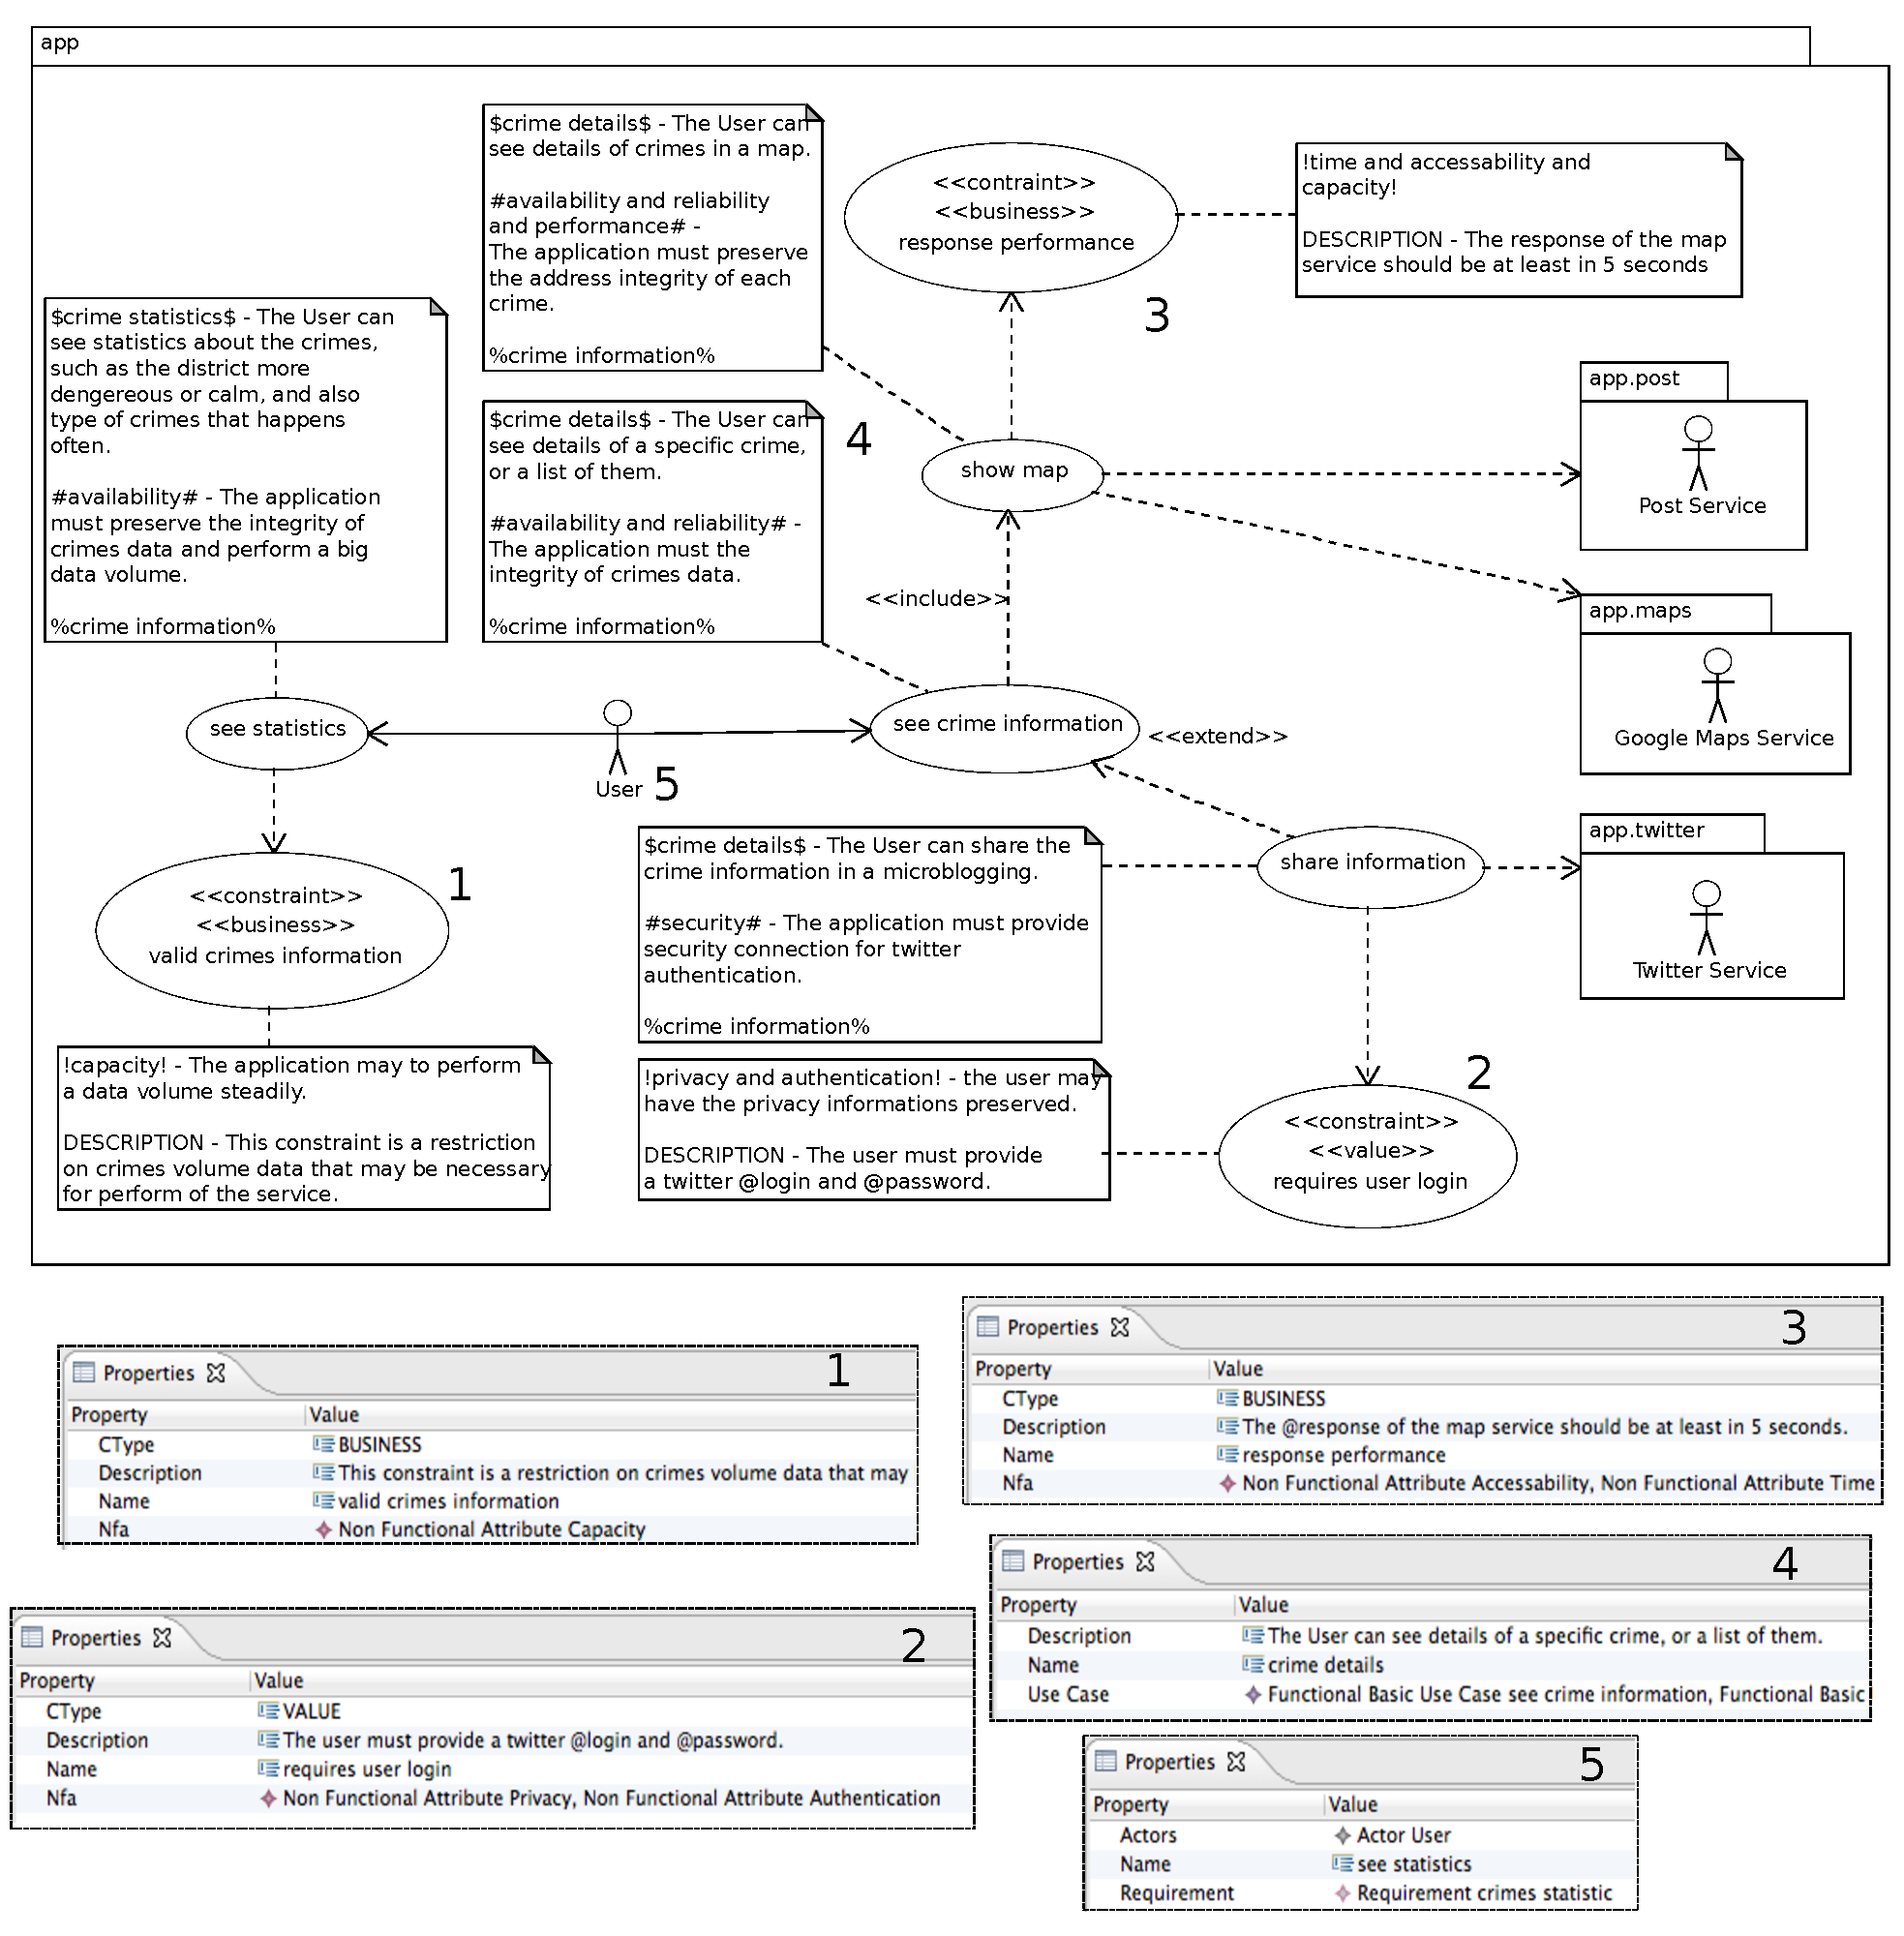
\includegraphics[width=0.99\textwidth]{chapters/validation/figs/crimes_useCase2}
\caption{\textit{See crime information} $\pi$-UseCase Detail.}
\label{fig:usecaseCrimeMap2}
\end{figure}  

Figure \ref{fig:usecaseCrimeMap2} describes the design of the use cases:
\textit{see crime information, see statistics, show map} and \textit{share
information}. To share information of a crime, it is necessary to access the
Twitter micro-blogging service to proceed with the authentication and posting.
The service requires the user id and password, however the
application must ensure the User privacy information while performing
authentication. To see statistics of crimes, the application should process a
larger volume of data to generate statistical results. Thus, it is required to
provide resources to ensure the data processing performance. The restriction on
map presentation is over response time and accessibility of the \textit{Postal}
and \textit{Google maps} services. The response time limit is 5 seconds. If the
map is not processed, only the information of the crime are presented. Figures
\ref{fig:usecaseCrimeMap1} and \ref{fig:usecaseCrimeMap2} also show the
properties used in the $\pi$SOD-M environment and the equivalent concepts in the
model.
 
\begin{figure}[ht!]   
\centering
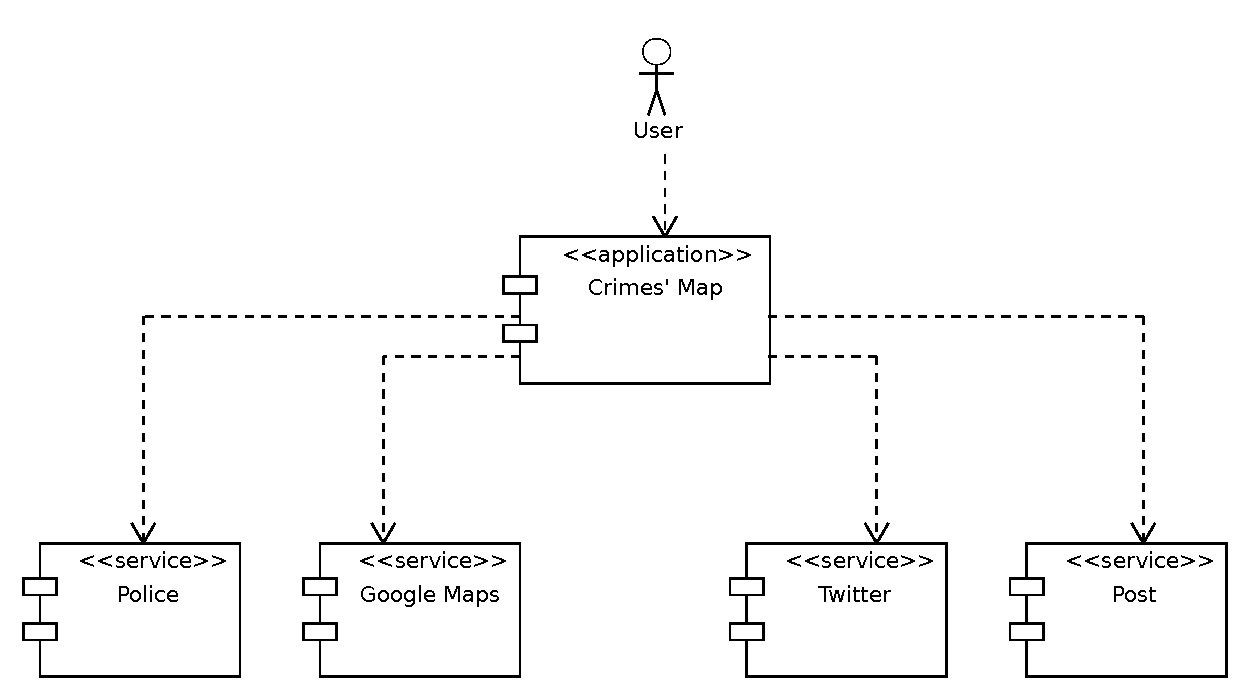
\includegraphics[width=0.8\textwidth]{chapters/validation/figs/crimesMap}
\caption{Crime Map Services.}
\label{fig:servicesCrimeMap}
\end{figure}
 
After the identification the various functions that are required by the system
to perform the business services, the $\pi$-ServiceProcess model is used to
represent the workflow necessary to perform a service within the system.
 
 
\subsection{$\pi$-ServiceProcess Model}
\label{sec:serviceprocess_crimesMap} 

The $\pi$-ServiceProcess model is used to represent the workflow necessary to
perform the system service. The service processes execution is described in two
steps. Figures \ref{fig:serviceProcessCrimeMap} and \ref{fig:serviceProcessCrimeMap2} show the
flow of functions execution described in the $\pi$-UseCase models shown
in Figures \ref{fig:usecaseCrimeMap1} and \ref{fig:usecaseCrimeMap2}. Each
diagram can represent different business services (see figures
\ref{fig:usecaseCrimeMap1} and \ref{fig:usecaseCrimeMap2}).

The diagrams of figures \ref{fig:serviceProcessCrimeMap} and
\ref{fig:serviceProcessCrimeMap2} were obtained by applying the
\textit{$\pi$-UseCase2$\pi$-ServiceProcess} transformation to the diagrams of
figures \ref{fig:usecaseCrimeMap1} and \ref{fig:usecaseCrimeMap2}, respectively.  

%  Thus, it makes easier to represent the performance of services. It is also possible to describe the
% process in a large workflow, but for applications running multiple
% services, it is better to have smaller processes to better represent the
% service execution. Thus we present the services business through the different
% processes as presented in Figures \ref{fig:usecaseCrimeMap1} and
% \ref{fig:usecaseCrimeMap2}.

\begin{figure}[ht!]   
\centering
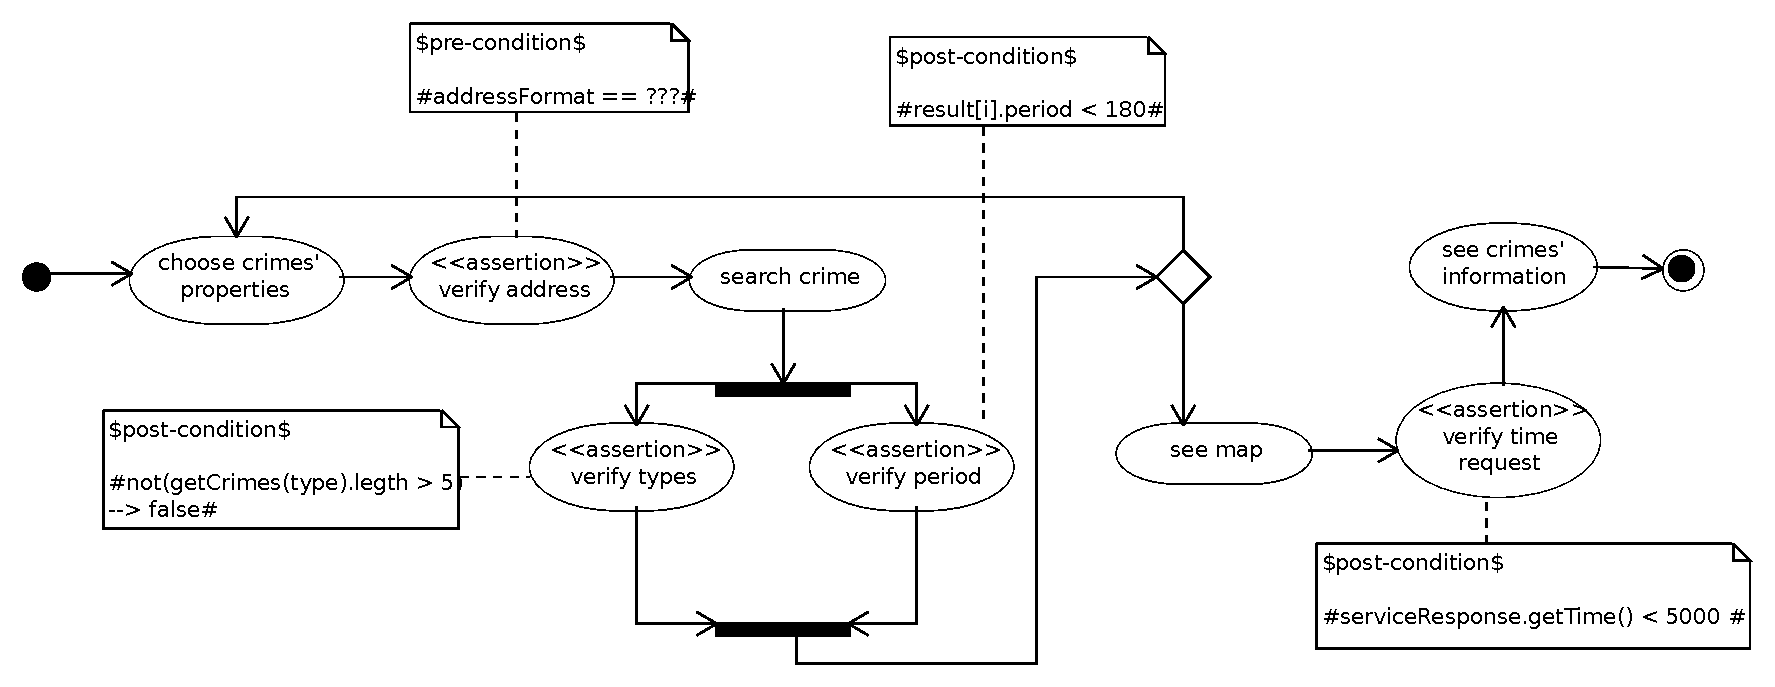
\includegraphics[width=0.99\textwidth]{chapters/validation/figs/model_piServiceProcess}
\caption{\textit{Crime information} $\pi$-ServiceProcess.}
\label{fig:serviceProcessCrimeMap}
\end{figure}  

\begin{figure}[ht!]    
\centering
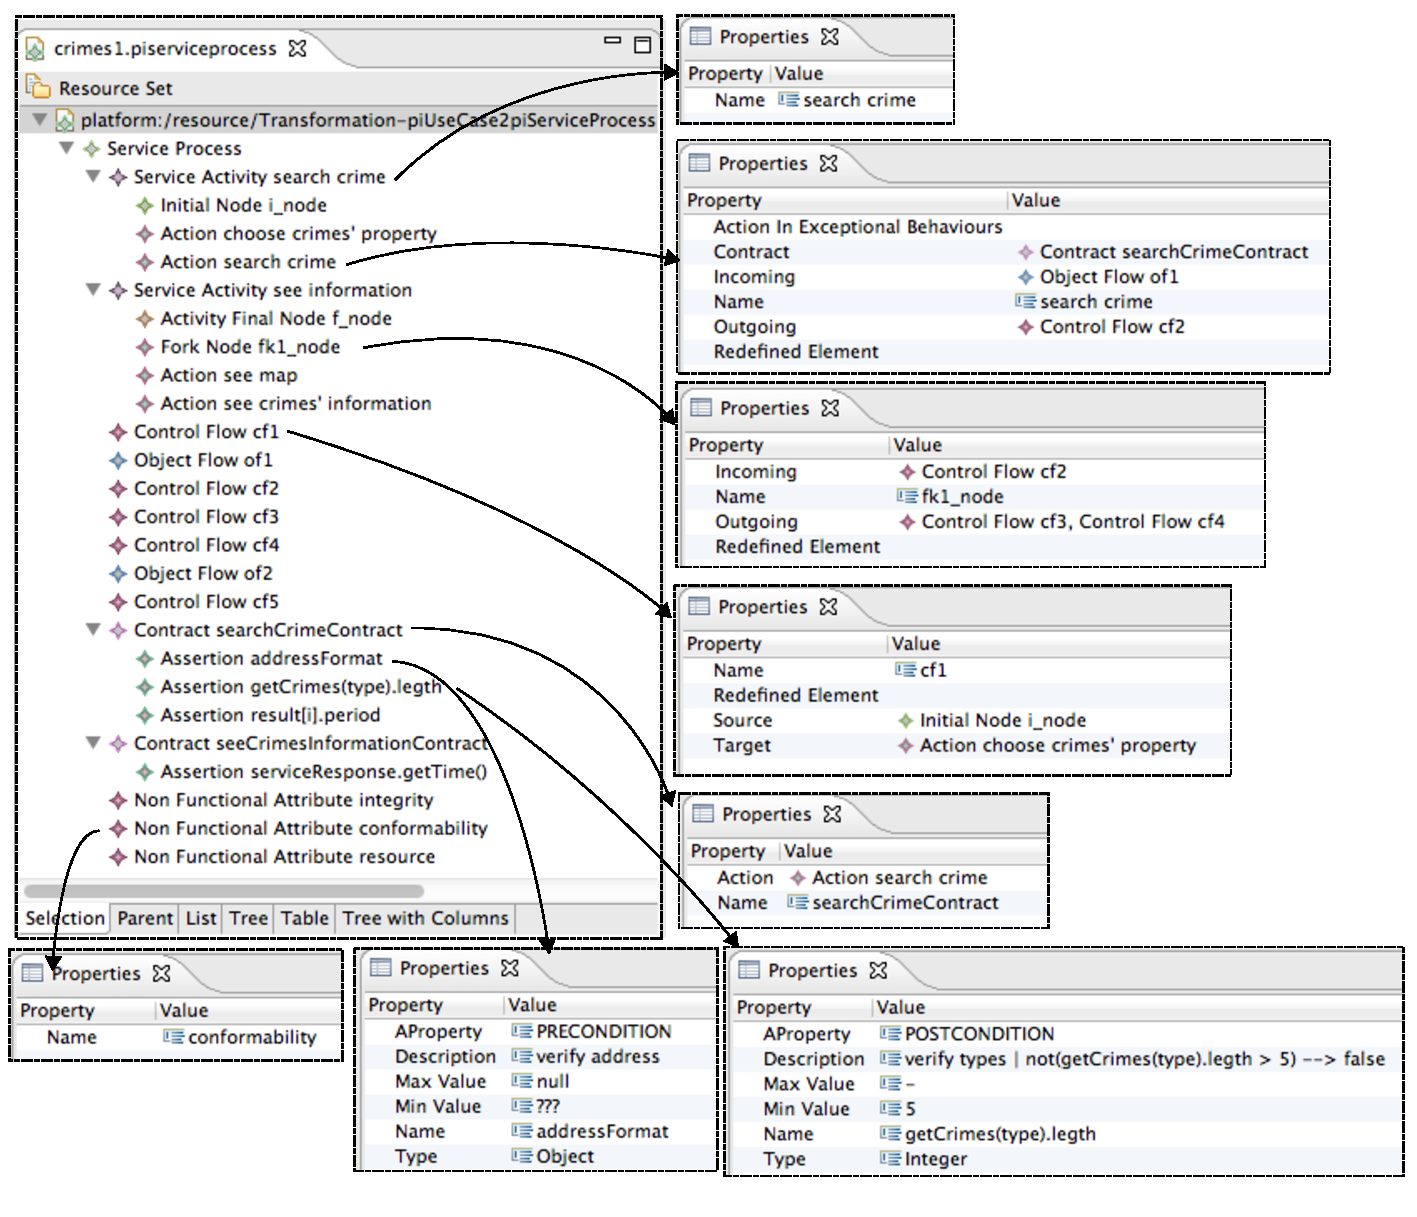
\includegraphics[width=0.99\textwidth]{chapters/validation/figs/toolServiceProcess_crime1}
\caption{\textit{Crime information}
$\pi$-ServiceProcess Environment.}
\label{fig:toolserviceProcessCrimeMap}
\end{figure} 

Each constraint of figures \ref{fig:serviceProcessCrimeMap} and
\ref{fig:serviceProcessCrimeMap2} are transformed into assertions. For example,
the assertions of address format,  crime types and time are restrictions over 
the action \textit{search crime}, being one pre-condition and two
post-conditions. These restrictions form the contract on the \textit{search
crime} function. Similarly, for viewing maps, if the answer to the request
takes longer than 5 seconds (5000 milliseconds), the map display is suspended and only 
the information is presented. Each assertion in this $\pi$-ServiceProcess model
stems from the $\pi$-UseCase model constraints. These restrictions are shown
in Figure \ref{fig:serviceProcessCrimeMap}. Figure
\ref{fig:toolserviceProcessCrimeMap} presents the equivalent model
generated by the methodology transformation in the $\pi$SOD-M environment for
the process detailed in Figure \ref{fig:serviceProcessCrimeMap}. Each node
defines the process element and its properties.

In Figure \ref{fig:toolserviceProcessCrimeMap}, \textit{i\_node} corresponds
to the initial process node. {\sc Actions} are grouped into  {\sc Service
Activities}, such as \textit{choose crimes property} action that is part of
the \textit{search crime} service activity. A {\sc Control Flow} is an edge that
links two nodes, for example \textit{cf1} connect the initial node
\textit{i\_node} (source) with the \textit{choose crimes property} action
(target). Figure \ref{fig:toolserviceProcessCrimeMap} also presents the
assertions described in Figure \ref{fig:serviceProcessCrimeMap} grouped into 
{\sc Contracts}. The contracts are: \textit{searchCrimeContract} and
\textit{seeCrimeInformationContract}. These contracts are related with the
actions \textit{search crime} and \textit{see crimes information}.

\begin{figure}[ht!]   
\centering
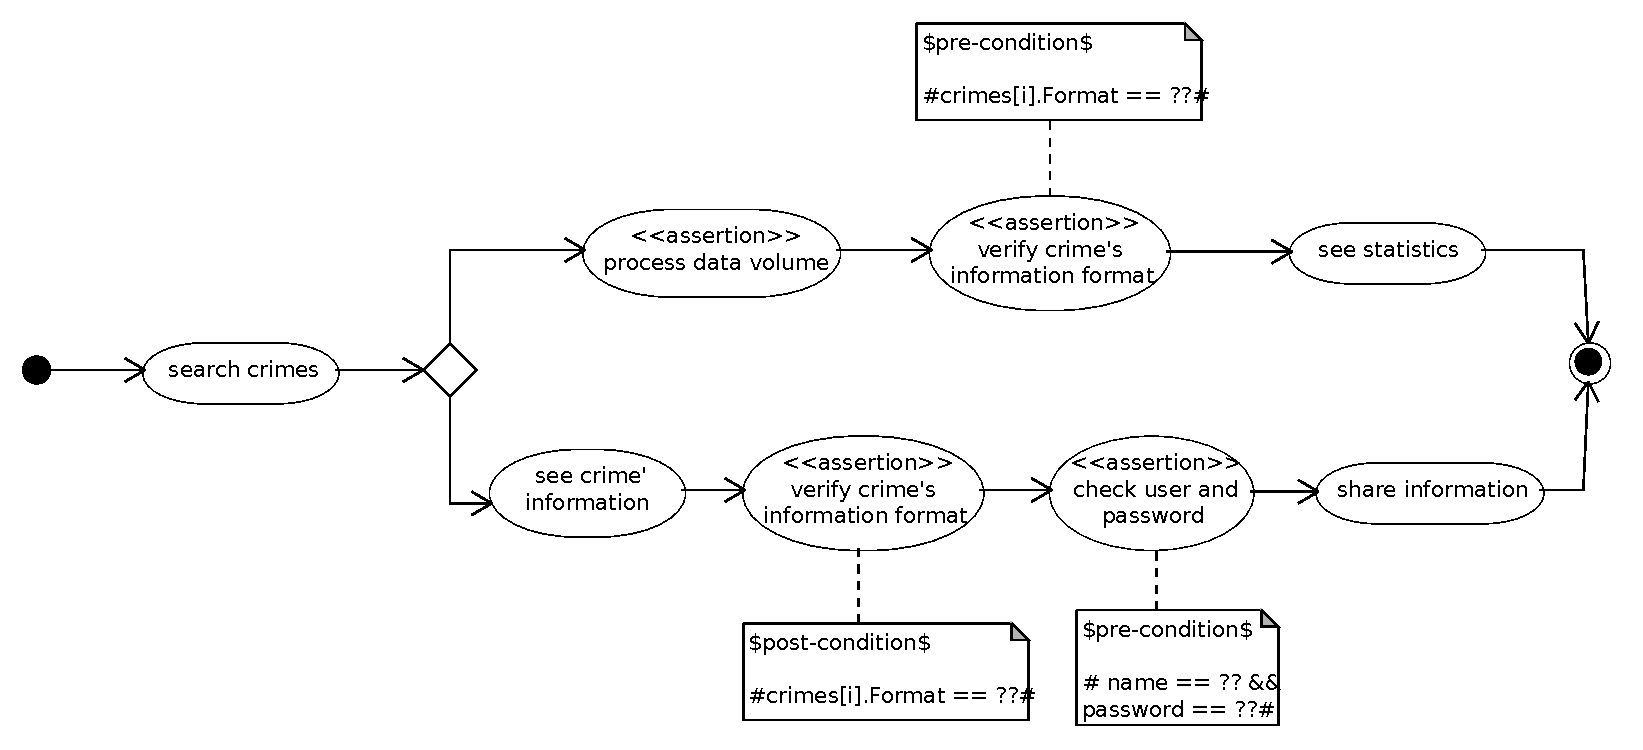
\includegraphics[width=0.99\textwidth]{chapters/validation/figs/model_piServiceProcess2}
\caption{\textit{See crime statistic and share information} $\pi$-ServiceProcess
Detail.}
\label{fig:serviceProcessCrimeMap2}
\end{figure}   


Figure \ref{fig:serviceProcessCrimeMap2} presents the assertions over the
 \textit{see statistics} and \textit{share information} actions. Both have 2 
pre-conditions. To \textit{share information} on Twitter it is necessary
to verify the format of crime information (140 characters) and the Twitter id
and password, for authentication. Regarding the \textit{see statistics} action, there is a
business restriction over data volume, and a value restriction over the crime
information format. Thus, the presentation of the crimes statistics must be done
after the contract verification. Figure
\ref{fig:toolserviceProcessCrimeMap2} presents the equivalent model
generated by the methodology transformation in the $\pi$SOD-M environment for
the process detailed in Figure \ref{fig:serviceProcessCrimeMap2}. Each node
defines the process element and its properties. Figure
\ref{fig:toolserviceProcessCrimeMap2} also presents the assertions grouped
into three contracts that are related with its specific actions. The contracts
are: \textit{seeStatisticsContract}, \textit{seeCrimeInformationContract} and
\textit{shareInformationContract}. The contracts are related with the action
\textit{see statistics}, \textit{see crimes information} and \textit{share
information}, respectively. 

\begin{figure}[ht!]    
\centering
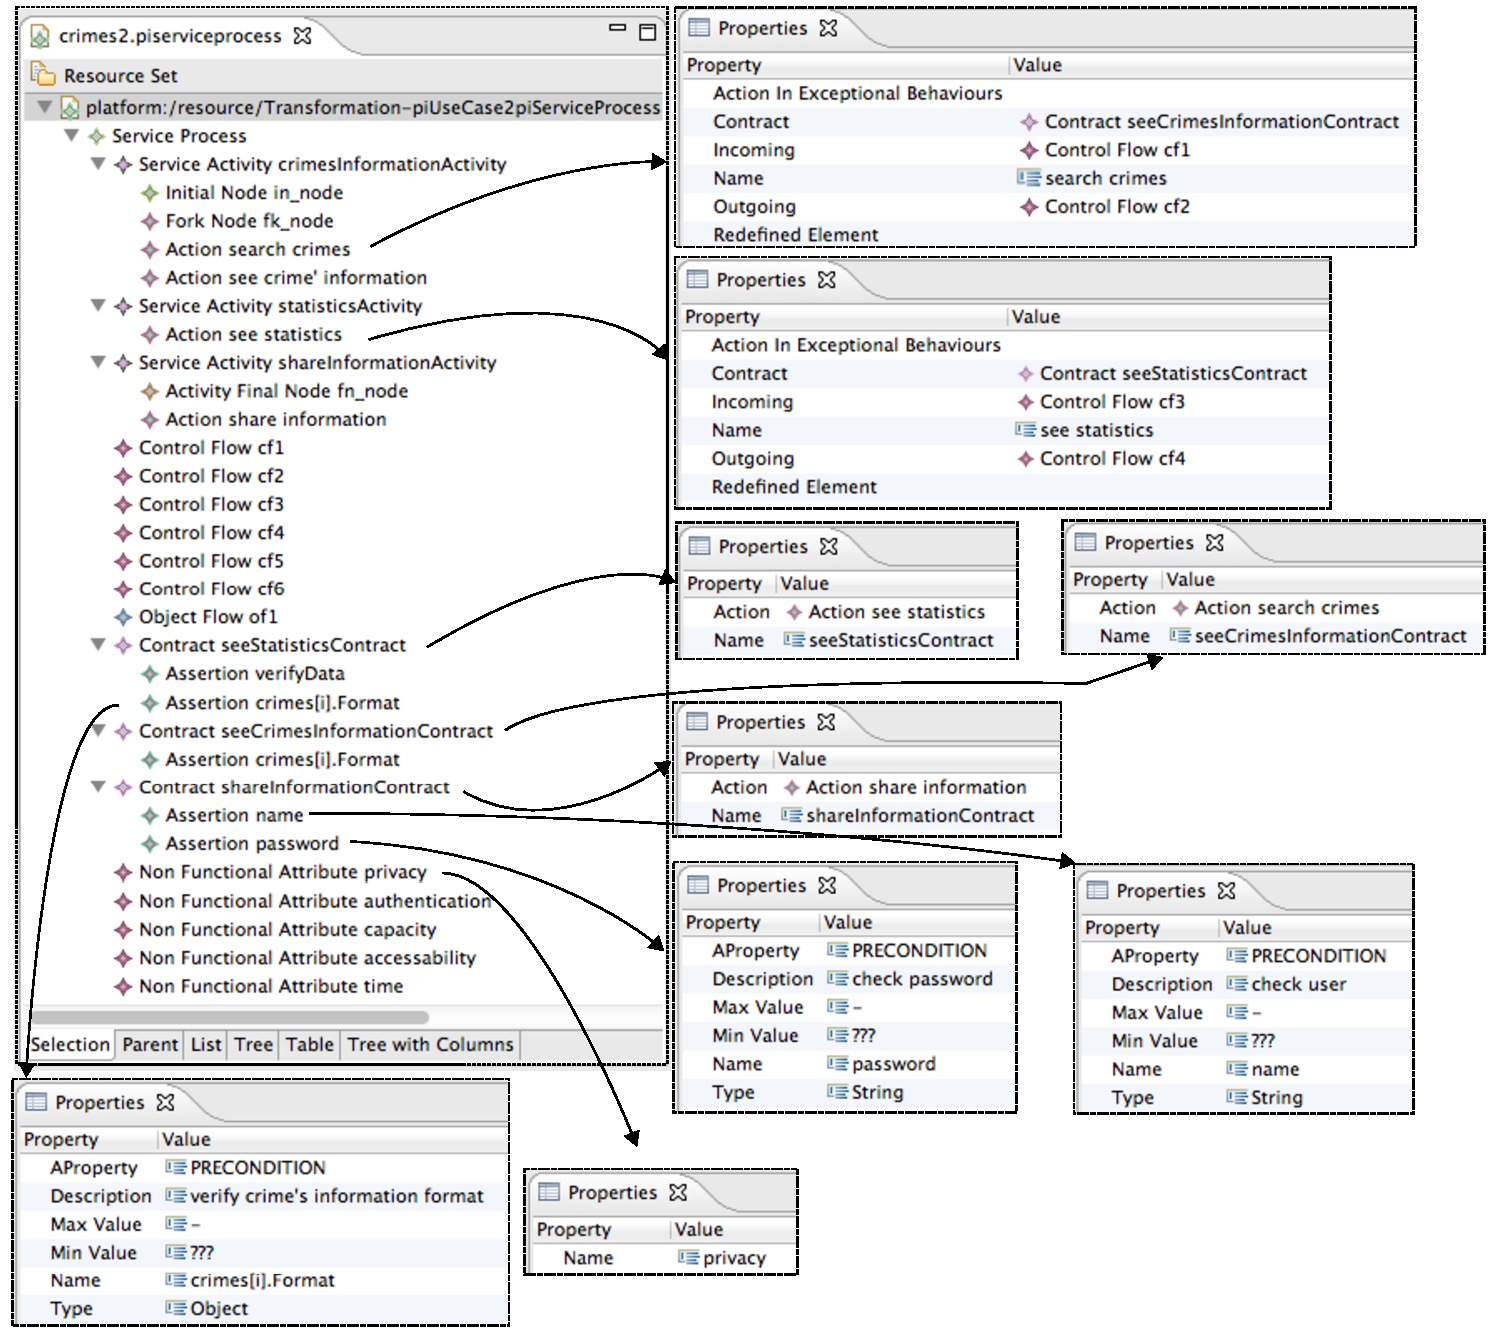
\includegraphics[width=0.99\textwidth]{chapters/validation/figs/toolServiceProcess_crime2}
\caption{\textit{Crime statistic and share information}
$\pi$-ServiceComposition Environment.}
\label{fig:toolserviceProcessCrimeMap2}
\end{figure} 


These models provide an overview of the business processes from the requirements
described in the $\pi$-UseCase model. These models also provide a more detailed
view of the execution of business processes and the possible
interaction with external services. The description of this interaction is the
result of the refinement of these models ($\pi$-ServiceProcess models) through
the $\pi$-ServiceComposition model.

\subsection{$\pi$-ServiceComposition Model}
\label{sec:servicecomposition_crimesMap} 

Figures \ref{fig:serviceCompositionCrimeMap} and
\ref{fig:serviceCompositionCrimeMap2} show the $\pi$-ServiceComposition models,
which represent the service composition processes of each
business service and additional indication of which are members of the business
that execute the action. Actions are derived from service activities,
identifying the set of actions that are necessary for the completion of each service.

The main partition expresses the \textit{Application} execution
(\textit{External false}) that represents the general process. Actions have the equivalent
service relation, which realize the external service, such as \textit{Police}, \textit{Google Maps} or
\textit{Twitter} services. They are expressed by a {\sc Business Collaborator}.
Both, Figure \ref{fig:serviceCompositionCrimeMap} and
\ref{fig:serviceCompositionCrimeMap2} present two external {\sc Business
Collaborators} describing the application services that are invoked. These
$\pi$-ServiceComposition models refine the $\pi$-ServiceProcess models, matching
action with real service functions that may be executed by the system
application. 

\begin{figure}[ht!]   
\centering
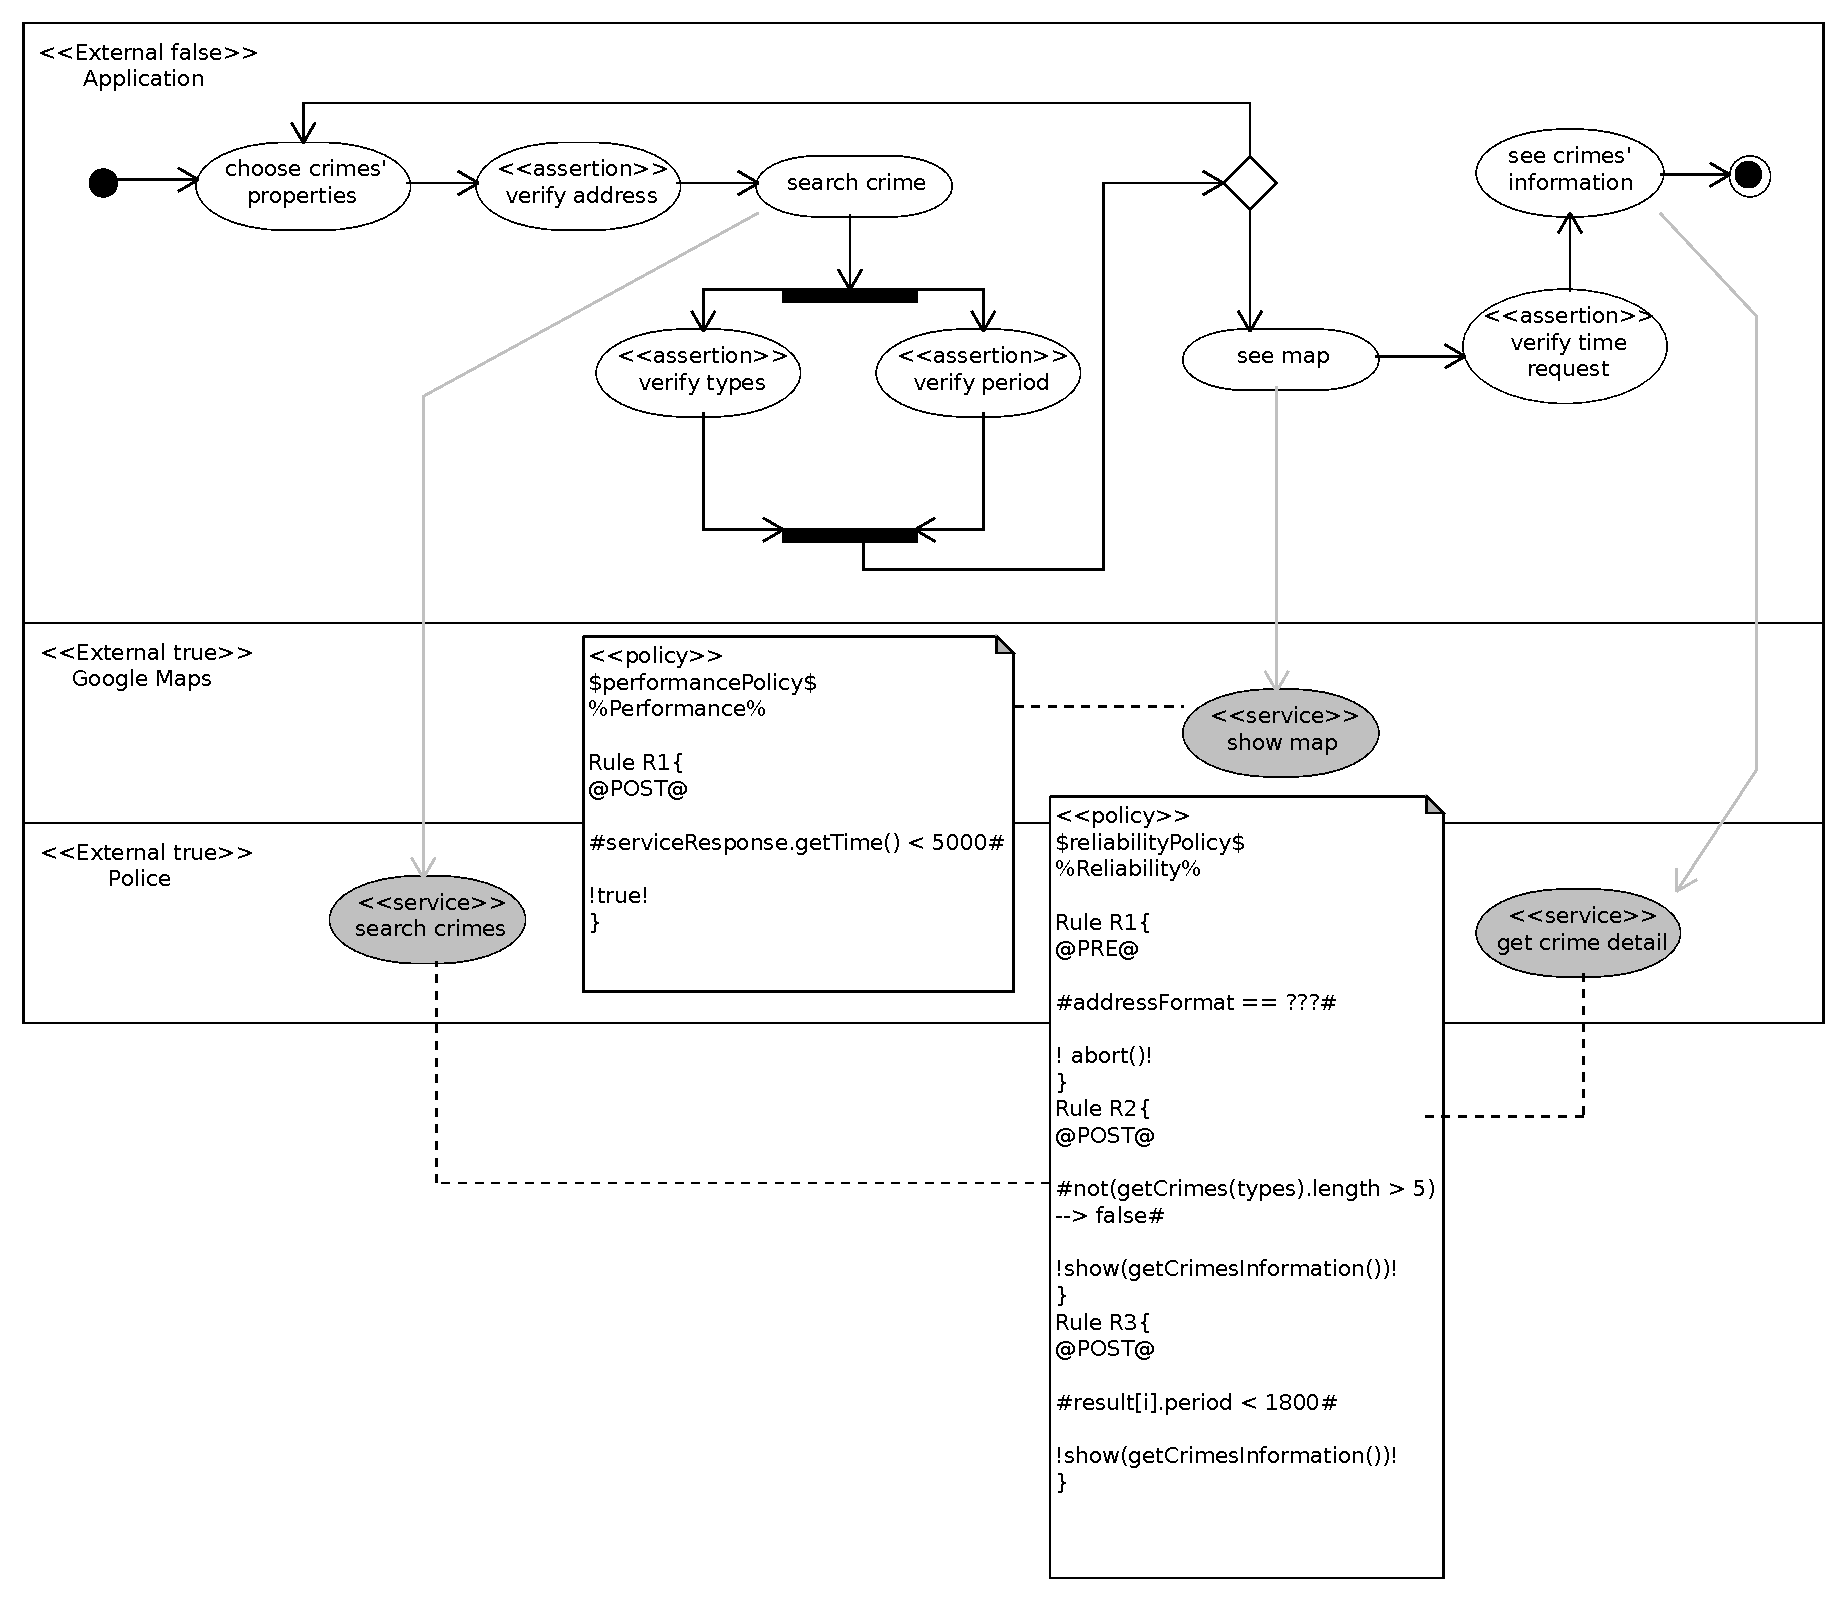
\includegraphics[width=0.99\textwidth]{chapters/validation/figs/model_piServiceComposition}
\caption{\textit{Crime information}
$\pi$-ServiceComposition.}
\label{fig:serviceCompositionCrimeMap} 
\end{figure} 


\begin{figure}[ht!]    
\centering
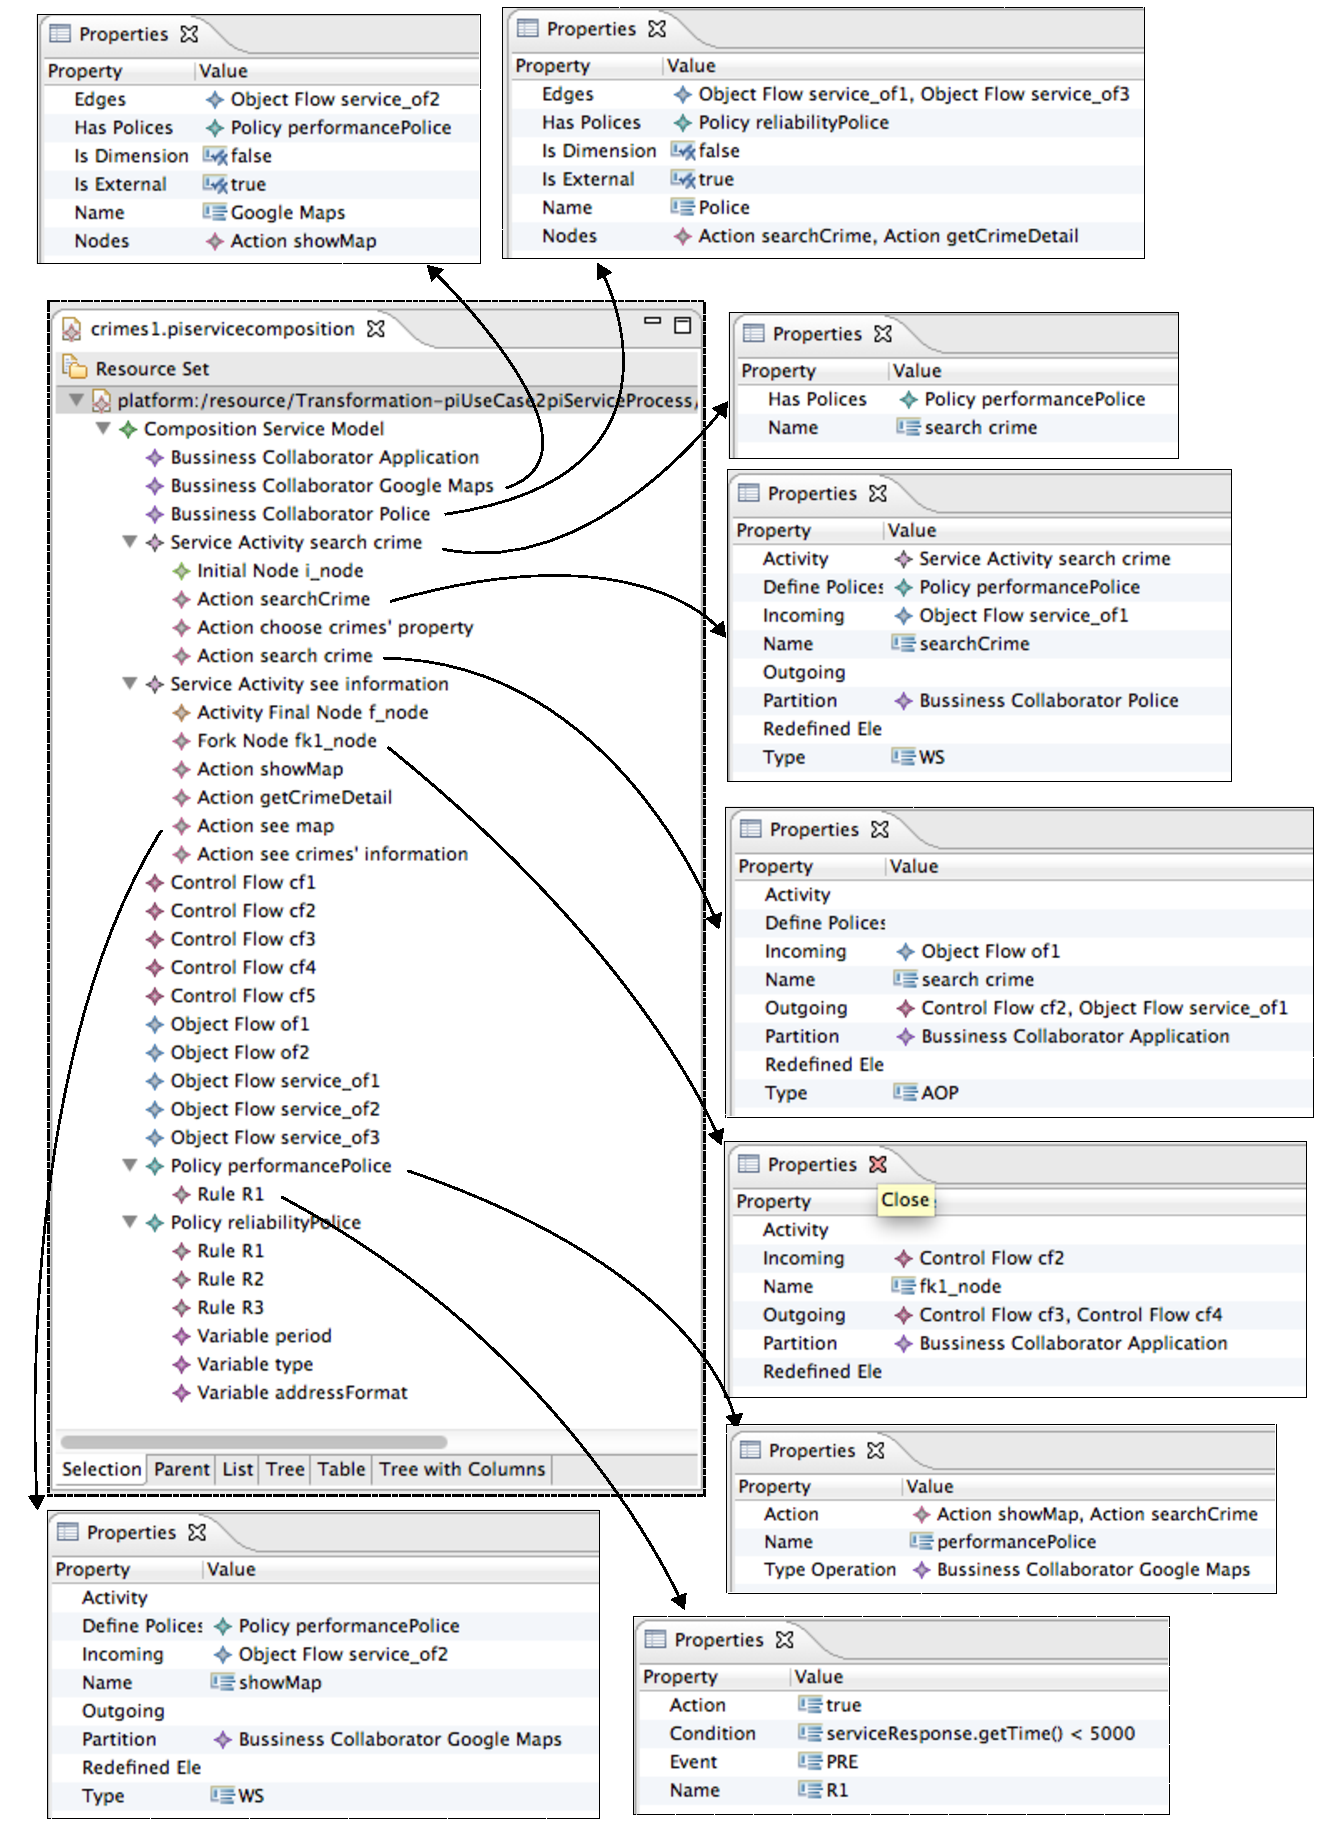
\includegraphics[width=0.99\textwidth]{chapters/validation/figs/toolServiceCOmposition_crime1}
\caption{\textit{Crime information}
$\pi$-ServiceComposition Environment.}
\label{fig:toolserviceCompositionCrimeMap}
\end{figure}  

For each $\pi$-ServiceComposition model, the contracts described in the
$\pi$-ServiceProcess model are grouped in policies. Figure
\ref{fig:serviceCompositionCrimeMap} describes the \textit{performancePolicy}
and \textit{reliabilityPolicy} policies, both associated with a service activity
and its actions. It is important to highlight that all policies are applied to the
entire actions associated with a service activity, for example, the
\textit{performancePolicy} verifies the request time for presenting the Google
maps. If the time exceeds 5000 milliseconds, the maps call is ignored and only
the crime information is presented. The \textit{reliabilityPolicy} is
associated with crime data verification. There are three rules over crime
address format, types of crime and the period of time in which it happens. The
crime presentation may obey the pre- and post-condition described in this policy. Figure
\ref{fig:toolserviceCompositionCrimeMap} presents the $\pi$SOD-M tool
description for the model described in Figure
\ref{fig:serviceCompositionCrimeMap}.

\begin{figure}[ht!]   
\centering
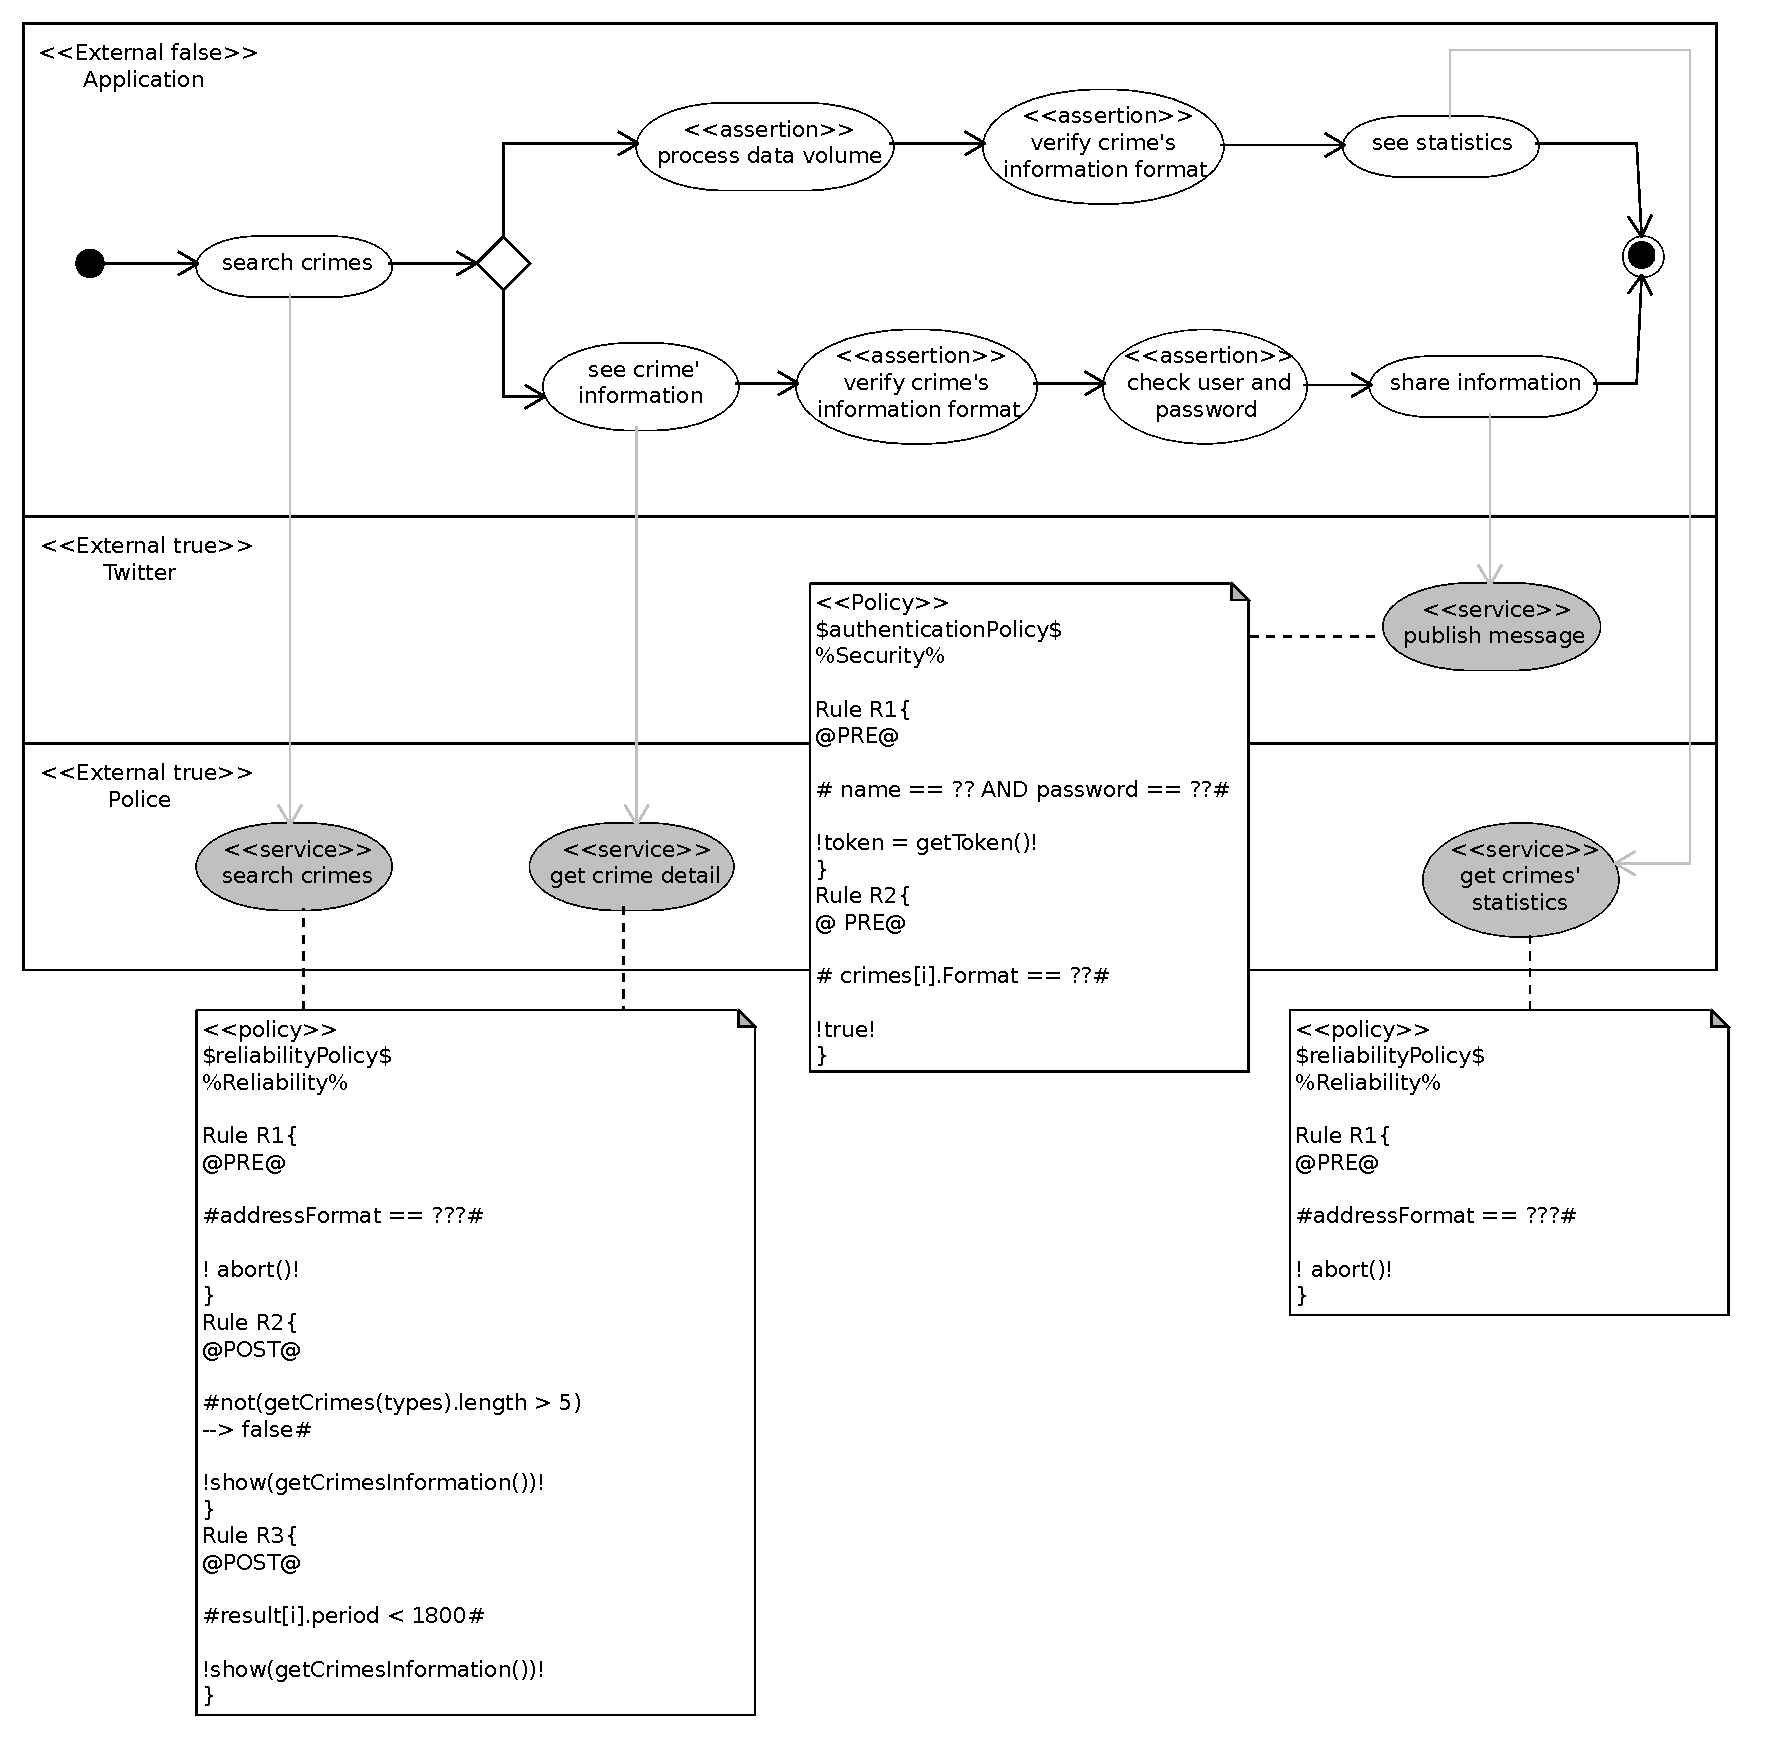
\includegraphics[width=0.99\textwidth]{chapters/validation/figs/model_piServiceComposition2}
\caption{\textit{Crime statistic and share information}
$\pi$-ServiceComposition.}
\label{fig:serviceCompositionCrimeMap2}
\end{figure}    

\begin{figure}[ht!]    
\centering
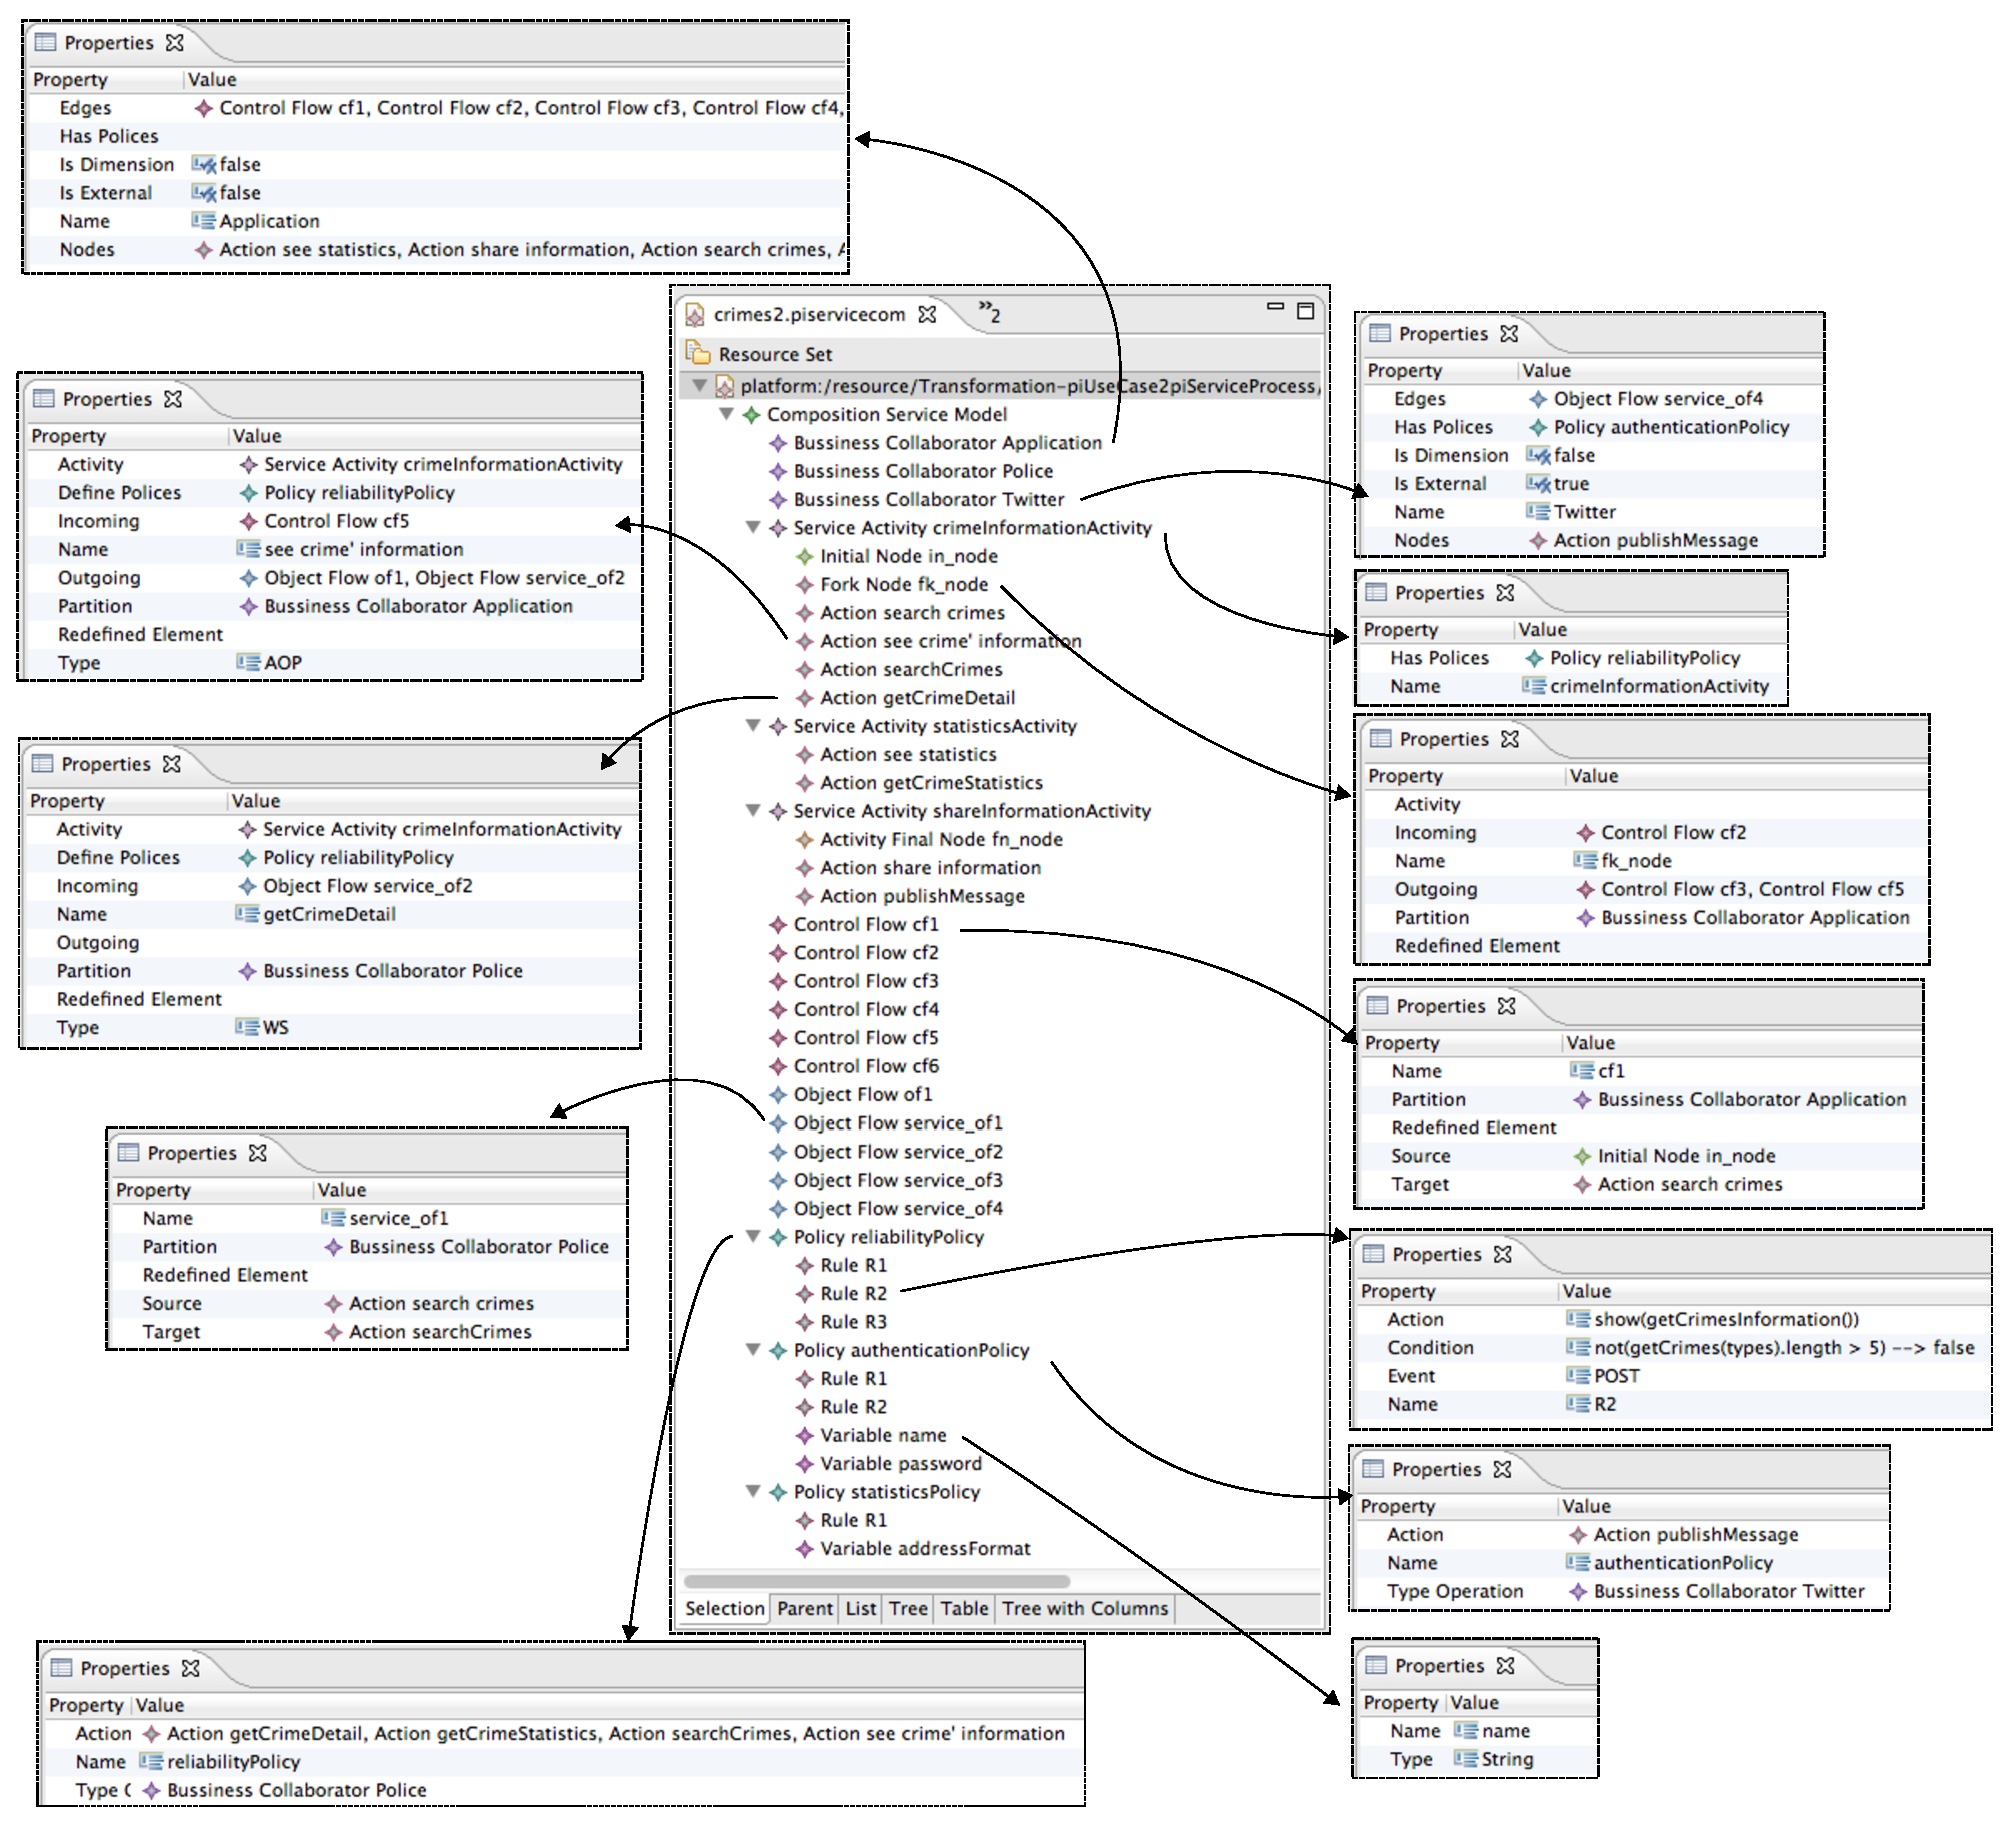
\includegraphics[width=0.99\textwidth]{chapters/validation/figs/toolServiceCOmposition_crime2}
\caption{\textit{See crime statistic and share information}
$\pi$-ServiceComposition Environment Detail.}
\label{fig:toolserviceCompositionCrimeMap2}
\end{figure}   

Figure \ref{fig:serviceCompositionCrimeMap2} refines the $\pi$-ServiceProcess
model described in Figure \ref{fig:serviceProcessCrimeMap2} and Figure
\ref{fig:toolserviceCompositionCrimeMap2} presents the $\pi$SOD-M tool
description for the model described in Figure
\ref{fig:serviceCompositionCrimeMap2}. This model details the policies for
\textit{crime statistic} and \textit{share information} services. The
policies are \textit{statisticPolicy} and \textit{authenticationPolicy},
respectively. 

These models provide an overview of the external services and its composition
from the actions described in the $\pi$-ServiceProcess model. These models also
provide a more detailed view of the system restrictions, applying policies
over external services. This model refines the $\pi$-ServiceProcess models
detailing the Business Collaborators that are expressed as external services,
and grouping contract into policies. 

% From these composition models, next
% step is generate the specification system code in $\pi$-PEWS.

% \subsubsection{$\pi$-PEWS Model}
% \label{sec:pews_crimesMap} 


\begin{figure}[ht!]
\tiny
\centering

\begin{lstlisting}[label=list:crimeInformationPEWS,caption=pi-PEWS
Specification: Crime information. ]

1  ns police =  "http:\\www.pm.rn.gov.br/service"
2  ns googleMaps =  "http://maps.googleapis.com/maps/api/"

4  alias chooseCrimesProperties = portType/chooseCrimesProperties in police
5  alias searchCrimes = portType/searchCrimes in police
6  alias seeMap = portType/showMap in googleMaps
7  alias seeCrimesInformation = portType/getCrimeDetail in police

9 (chooseCrimesProperties . searchCrimes)* . seeMap . seeCrimesInformation

11 def contract searchCrimesContract{
12  isAppliedTo: searchCrimes;    
13  requires: addressFormat == ?? 
14     (onFailureDo: call(chooseCrimesProperties) );  
15    ensures : !(getCrimes(types).length > 5) ==> false &&
16              result[i].period < 1800
17       (onFailureDo: show(getCrimesInformation())); 
18 }

20 def contract showMapContract{
21  isAppliedTo: seeMap;    
22    ensures : serviceResponse.getTime() < 5000
23       (onFailureDo: skip); 
24 }
\end{lstlisting}
\label{fig:crimeInformationPEWS}  
\end{figure}  


The result of the transformation of this model to the \textit{$\pi$-PEWS} model
is gives in the listing \ref{list:crimeInformationPEWS} and
\ref{list:crimeStatisticsPEWS}.


\begin{figure}[ht!]
\tiny
\centering
\begin{lstlisting}[label=list:crimeStatisticsPEWS,caption=pi-PEWS Specification: Crime
statistic and share information. ]

1  ns police =  "http:\\www.pm.rn.gov.br/service"
2  ns twitter =  "https://dev.twitter.com/docs/api/"

5  alias searchCrimes = portType/searchCrimes in police
7  alias seeCrimesInformation = portType/getCrimeDetail in police
4  alias seeStatistics = portType/getCrimeStatistics in police
6  alias shareInformation = portType/publishMessage in twitter

9  searchCrimes . ((seeCrimesInformation . shareInformation) |
10					seeStatistics)

12 def contract searchCrimesContract{
13  isAppliedTo: searchCrimes;    
14  requires: addressFormat == ?? 
15     (onFailureDo: call(chooseCrimesProperties) );  
16    ensures : !(getCrimes(types).length > 5) ==> false &&
17              result[i].period < 1800
18       (onFailureDo: show(getCrimesInformation())); 
19 }

21 def contract shareInformationContract{
22  isAppliedTo: shareInformation;    
23  requires: name == ?? AND password == ?? &&
24              crimes[i].Format == ?? 
25     (onFailureDo: call(shareInformation) );  
26 }

28 def contract seeStatisticsContract{
29  isAppliedTo: seeStatistics;    
30  requires: crimes[i].Format == ?? 
31     (onFailureDo: call(seeStatistics) );  
32 }
\end{lstlisting}
\label{fig:crimeStatisticsPEWS}  
\end{figure}  


  

\section{Example 3: GesIMED Application}
\label{sec:siw_gesimed}

Aiming to perform a qualitative analysis and the validation of $\pi$SOD-M
methodology, we present the \textit{GesIMED Application}\footnote{If necessary, a detailed description of this case
 study can be found in \cite{valeriaThesis}.}
 case study.  

% This case
% study was described in~\cite{valeriaThesis} with the goal of validating the
% SOD-M methodology. In
% this section we present the different produced by using the SOD-M and
% $\pi$SOD-M, as well as the contributions generated by of our proposal. We will
% model the same business case for both methods and see the difference between them.

This \correctingText{example} was originally developed in \cite{valeriaThesis} for the SOD-M
methodology. Here , we adapt the requirements of the system to include NFR. This
system is a management Web system that processes medical images through the Web \cite{valeriaThesis}. The objective is to
manage information about the creation and maintenance of scientific studies
for neuroscience research. The application is designed to be used primarily by
researchers in neuroscience, such as neurologists, neuropsychologists and
neuroradiologists who conducting research in this area.

The application requirements are the following: (i) a
database of medical images that can be accessed by the user; (ii) it has an
interface for querying the database; (iii)  implement standard  procedures for analyzing
and processing stored images; and (iv) the images analysis and processing
results must be also stored, so they can be used in future studies. 

The  Medical Image Analysis Laboratory from the Universidad Rey Juan Carlos
(LAIM) offers three specific services to researchers in neuroscience. The access
to services has a cost and financial revenues are assigned to LAIM. The services
are:

\begin{itemize}
  \item Storage and retrieval medical imaging service (SACim);
  \item Image processing service (SPim);
  \item Image visualization service (SVim);
\end{itemize}

From the functions offered by these services we will detail the application
characteristics. The application uses these services offered by LAIM for
modeling the application. 

% From this case study description we present the modeling performed in SOD-M, and
% soon after perform the modeling in $\pi$SOD-M. From the business case
% \textit{perform image processing}, we will differentiate the characteristics of
% each methodology.


  
% \subsection{$\pi$SOD-M Modeling}
% \label{sec:GesIMED-pisodm}
\bigskip
\bigskip
 
Given the description of the business requirements and the expected
functionality of the system, $\pi$SOD-M is used for developing this application. 

% The modeling of \textit{GesIMED} application in $\pi$SOD-M has
% the same input considered in SOD-M method, the description of business
% requirements and system functionality. Thereafter, we follow the development of
% each model according to specification of the $\pi$SOD-M  methodology. Our goal
% in this section is to highlight the particularities of $\pi$SOD-M regarding
% SOD-M.



We will detail the \textit{perform image processing} business service. In $\pi$SOD-M, the \textit{$\pi$-UseCase} model
describes the application functions, restrictions and its non-functional
attributes. This business service (\textit{perform image processing}) is 
sufficiently rich to describe the peculiarities of $\pi$SOD-M
compared to the original model of SOD-M. 

\subsection{\textit{$\pi$-UseCase} Model}

Figure \ref{fig:piUseCase-imageProcessing} shows the \textit{$\pi$-UseCase}
model. This model defines four constraints: \textit{authenticate, response time,
data format} and \textit{validate payment card}. These constraints are restrictions over the functions of the
\textit{GesIMED} application. In the description of each constraint it is
necessary to describe the constraint type (\textit{business} or \textit{value}).
The model has one business constraint and three value constraints. It is
possible to describe constraints for each use case application.


\begin{figure}[ht!]
\centering
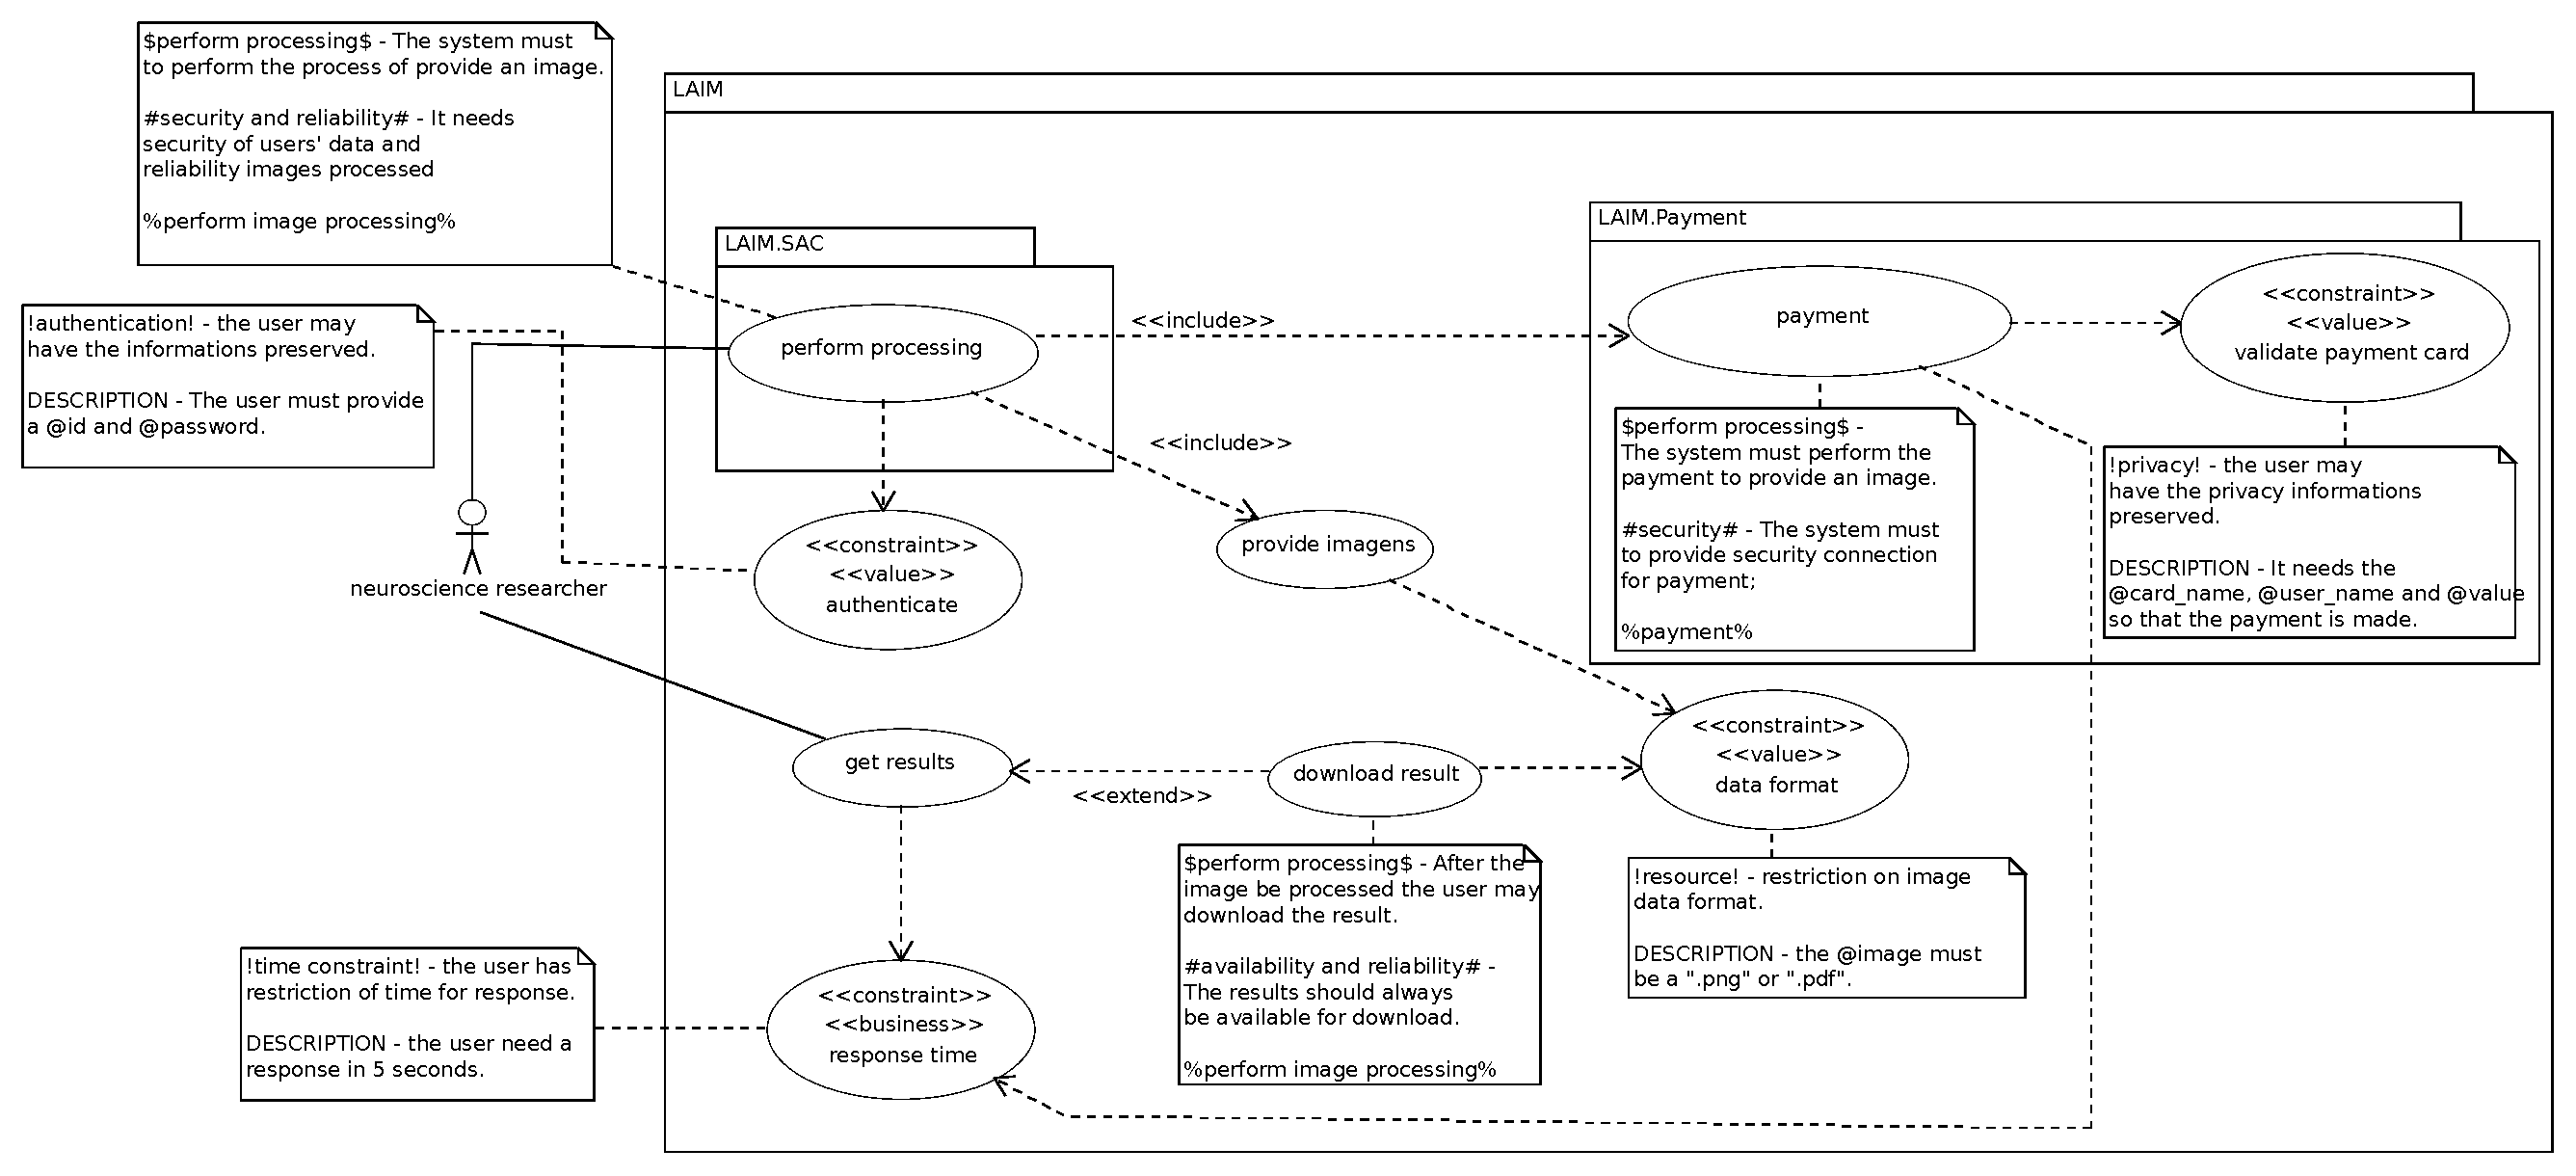
\includegraphics[width=.99\textwidth]{chapters/validation/figs/neuro-piuc-01.pdf}
\caption{$\pi$-UseCase: Perform Image Processing.}
\label{fig:piUseCase-imageProcessing}
\end{figure} 

% Notice that the other use cases are the same of those that were
% modeled in SOD-M. The difference is that they are now systematized in packages.
% Our approach guides the systematic functions through packages, because these
% packages represent business collaborators.

Besides the constraints, the model details the non-functional attributes
related to each constraint, for example, the \textit{response time} constraint.
For value constraints, it is necessary identify candidates variables to be
verified, through the use of \textit{@}. For example, the
authentication constraint, has the \textit{@id} and \textit{@password}
identifiers that must be verified. 

% It is possible to identify a real difference between the use case models in
% SOD-M and $pi$SOD-M, especially with regard of constraints, in a way to describe
% details of quality requirements.  


\begin{figure}[ht!]
\centering
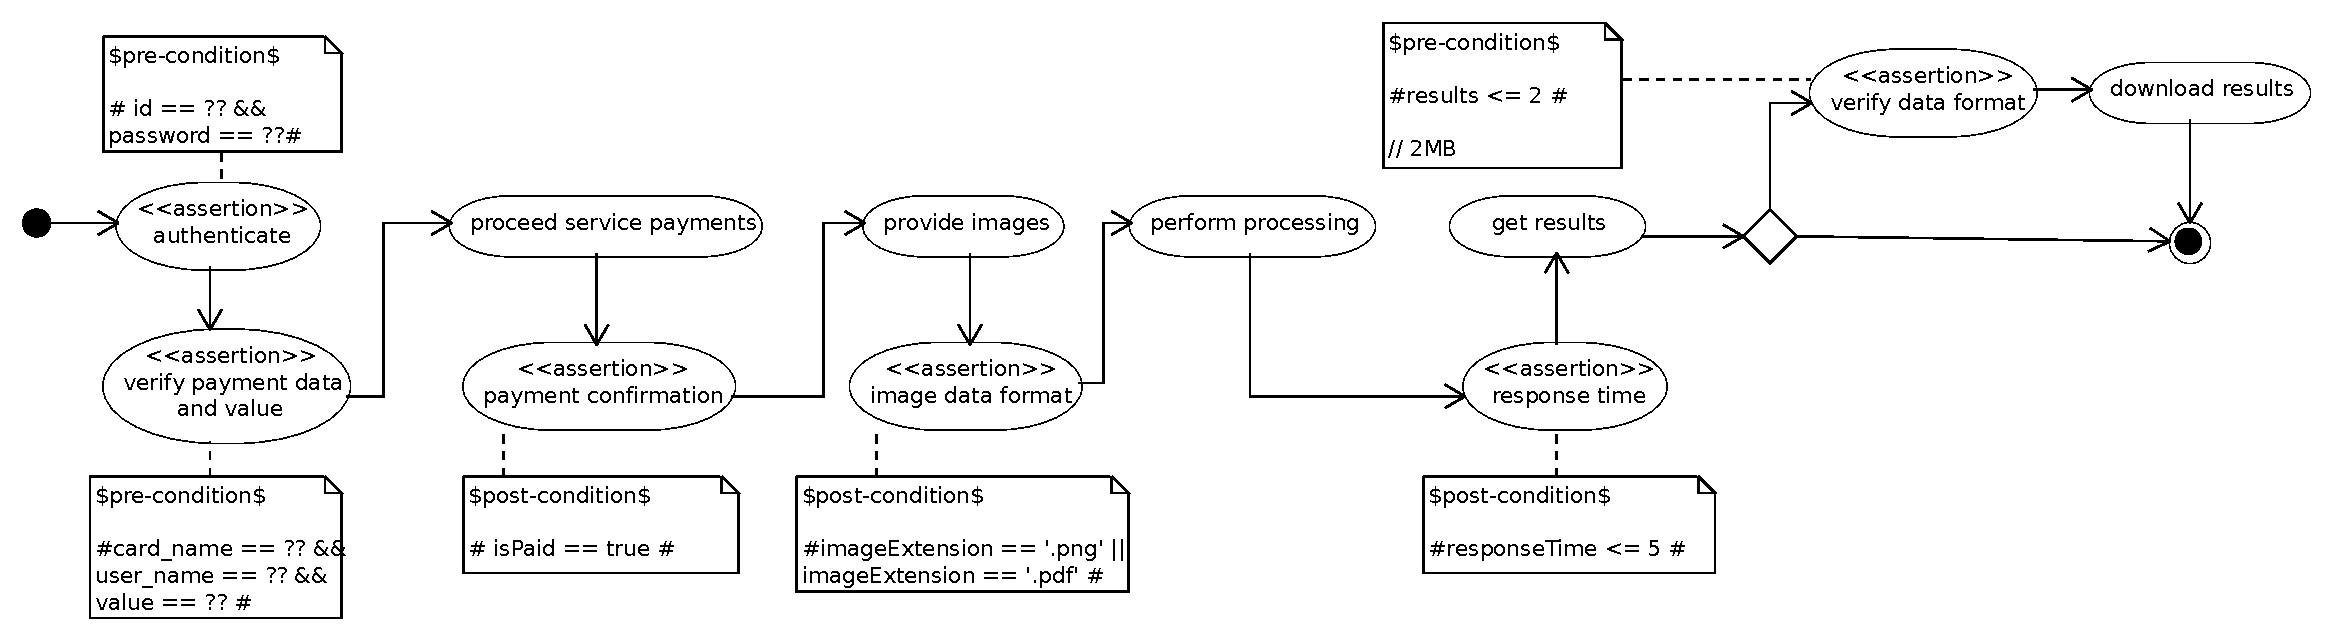
\includegraphics[width=.99\textwidth]{chapters/validation/figs/neuro-pisp-01.pdf}
\caption{$\pi$-ServiceProcess: Perform Image Processing.}
\label{fig:piServiceProcess-imageProcessing}
\end{figure} 

The main feature of our approach is the association of non-functional
requirements with use cases. For example, the user can identify that the
quality requirement related to a payment process is
\textit{transactional} or \textit{data privacy}. So, through the process, it is
possible to refine this information, considering other details provided.

The result of the \textit{$\pi$-UseCase} model is a detailed list of
constraints, its respective use case, system requirement information and
non-functional attributes required for each service.

\subsection{\textit{$\pi$-ServiceProcess} Model}

Figure \ref{fig:piServiceProcess-imageProcessing} shows the
\textit{$\pi$-ServiceProcess} model. This model transforms the use cases into actions,
and constraints into assertions. The resulting workflow describes pre or
post-conditions on workflow execution. The assertions are wrappers around the
action. All the assertions related to a specific action become a
contract. For example, the \textit{proceed payments service} action has a
pre- and a post-condition. The pre-condition is a restriction over the payment
information (\textit{card number, name} and \textit{value}), while the
post-condition defines the final state after the payment. The other assertions
of this model are the result of the transformation of each constraint described
in the \textit{$\pi$-UseCase} model. 
 
%  Notice that the workflow (figure \ref{fig:piServiceProcess-imageProcessing})
%  is the same as described in SOD-M, with the difference of having assertions
%  during the process, so that the constraints are verified.
 
 \begin{figure}[ht!]
\centering
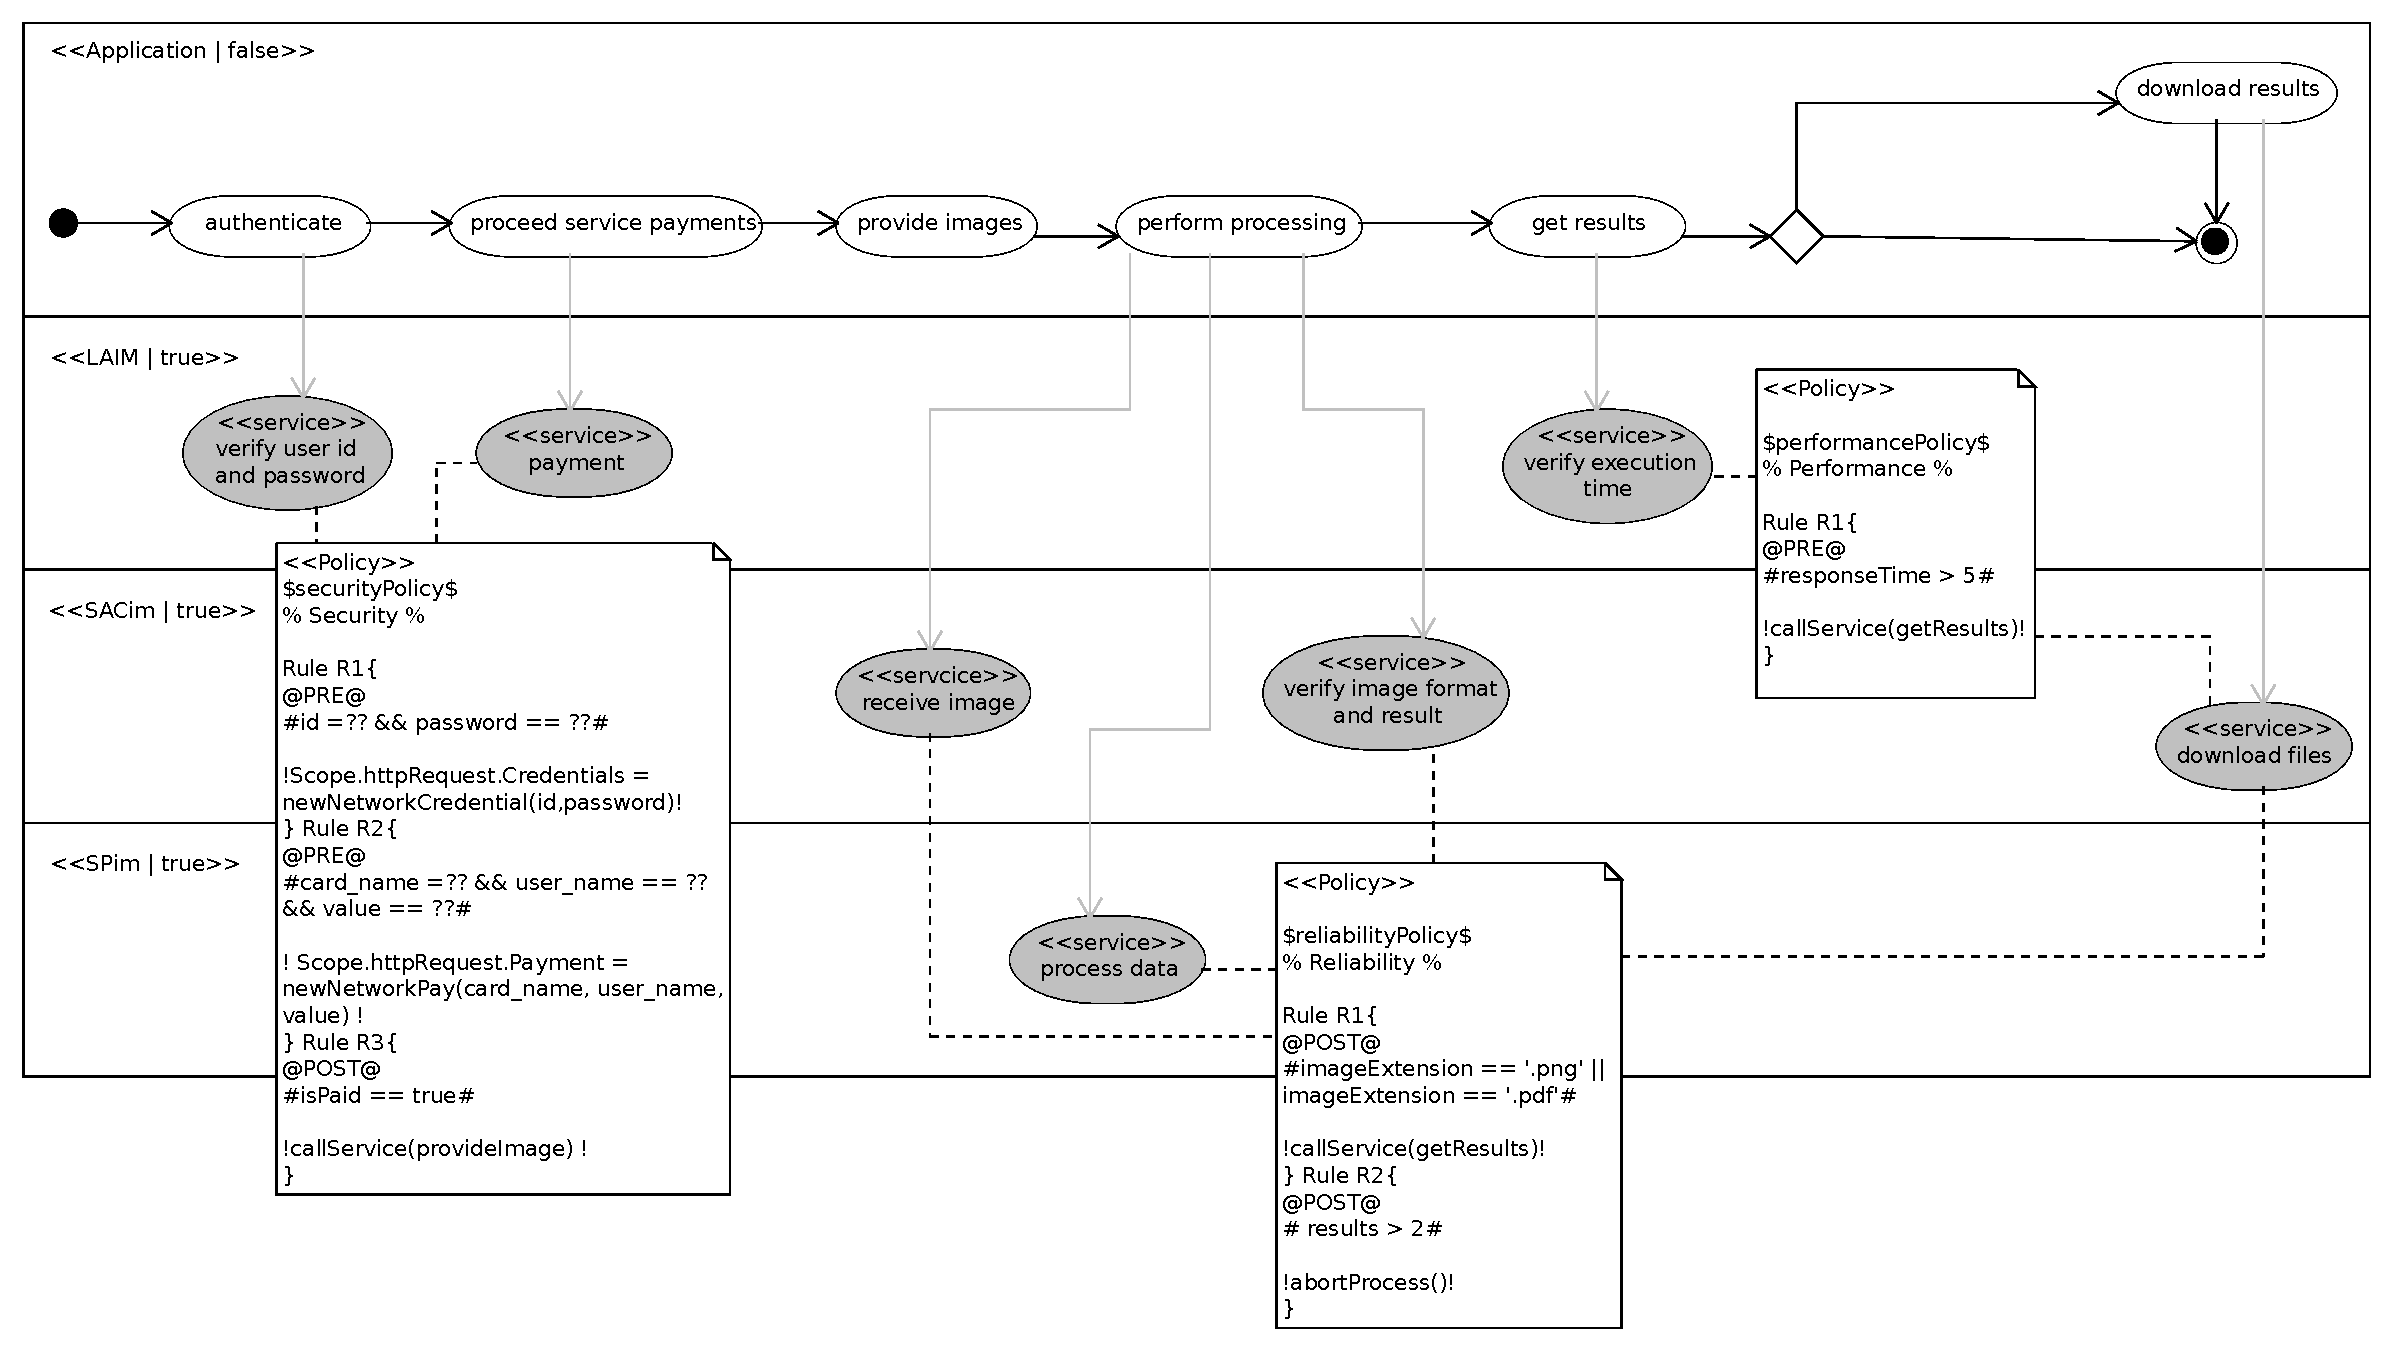
\includegraphics[width=.99\textwidth]{chapters/validation/figs/neuro-pisc-01.pdf}
\caption{$\pi$-ServiceComposition: Perform Image Processing.}
\label{fig:piServiceComposition-imageProcessing}
\end{figure} 

\subsection{\textit{$\pi$-ServiceComposition} Model}

The \textit{$\pi$-ServiceComposition} model presented in figure
\ref{fig:piServiceComposition-imageProcessing} refines the 
\textit{$\pi$-ServiceProcess} model. This model
describes the real services and their associated collaborators. The information
of the business collaborator comes from the package description. Contracts with
the same non-functional requirements become service policies. The policies
define rules, which are a direct transformation of the assertions in the
previous model.

% Another difference
% of our approach to the original approach of SOD-M, is that we do not treat each
% collaborator as a business process. 
 
\begin{figure}
\tiny
\centering

\begin{lstlisting}[label=list:pewsNeuro,caption=pi-PEWS Specification: Perform
Image Processing. ]

1  ns app =  "http:\\www.neuro.laim.org"
2  ns LAIM =  "http:\\www.neuro.laim.org/laim-service.wsdl"
3  ns SACim = "http:\\www.neuro.laim.org/sacim-service.wsdl"
4  ns SPim =  "http:\\www.neuro.laim.org/spim-service.wsdl"

6  alias authenticate = portType/verifyUserandPassword in LAIM
7  alias proceedServicePayment = portType/payment in LAIM
8 alias provideImage = portType/provideImage in app
9  alias receiveImage = portType/receiveImage in SACim
10 alias processData = portType/processData in SPim
11 alias verifyImageFormatAndResult = portType/verifyImageFormatAndResult in
12 SACim alias getResults = portType/verifyExecutionTipe in LAIM
13 alias downloadResults = portType/downloadFiles in SACim

15 service performProcessing = 
16            receiveImage . processData . verifyImageFormatAndResult

18 authenticate . proceedServicePayment . provideImage . 
19   performProcessing . [act(getResults).time > 5]getResults .
20   {downloadResults}

21 def contract authenticateContract{
22  isAppliedTo: authenticate;    
23  requires: id == ?? && password = ??;
24     (onFailureDo: call(authenticate) )  
25 }

27 def contract paymentContract{
28  isAppliedTo: proceedServicePayment;    
29  requires: card_name =?? && 
30  			user_name == ?? && 
31  			value == ??;  
32  ensures : isPaid == true ;
33 }

35 def contract performProcessingContract{
36  isAppliedTo: performProcessing;    
37  requires: imageExtension == '.png' || imageExtension == '.pdf'
38    (onFailureDo: skip );    
39  ensures : resultValue <= 2 ;
40 }
\end{lstlisting}
\label{fig:pewsNeuro}  
\end{figure}  



Listing \ref{list:pewsNeuro} shows the \textit{$\pi$-PEWS} specification that
was generated from the \textit{$\pi$-ServiceComposition} model. This
specification considers the operations (lines 6-16), its business collaborators
(namespaces in the lines 1-4), the main workflow (lines 18-20) and services
restrictions (described as contracts in the lines 21-40). The final result of
our approach is the specification that describes the structure and sequence of
execution to be performed by an orchestrator. \textit{$\pi$-PEWS}
specification defines a set of contracts to represent the application restrictions. Thus,
using $\pi$SOD-M it is possible to refine the models until the code generation.
 
\section{Lessons Learned}
\label{sec:leassonsLearned}

This section summarizes the experience we obtained after the use of $\pi$SOD-M
for the three \correctingText{examples}. \newText{In this section we also present some
results collected from the evaluation made ​​between the two approaches.}

\subsection{Example 1: To Publish Music} 
 
In this case study we can see that the restrictions on web services can be
modeled from the early stages of development, not leaving it to the programming
language, or to the programmer to resolve this type of problem. More
specifically, this case study had restrictions \textit{performance} and \textit{security}. Since
the \textit{$\pi$-UseCase} model to the \textit{$\pi$-ServiceComposition} model,
non-functional requirements and their attributes might be described without
serious impact on the modeling of other application requirements.  

The restrictions on the functions provided by
the \textit{Spotify} service was basically \textit{performance}. This type of
restriction is not easy to represent in the implementation, because it relies on
the network available to the user. We described the
constraints and refined them into a \textit{ performance} policy for updating
the music. The security restrictions have been described for the service that provides banking information. The security policy generated was described
for two functions of the Bank service, \textit{pay} and \textit{send
confirmation} functions. This type of specification can be refined incrementally
by applying the modelling steps defined by the $\pi$SOD-M methodology.

\correctingText{It} does not cover all the possible restrictions in
an application but it shows that it is possible to guarantee
quality requirements refining information at each iteration of the modeling,
such as constraints of \textit{performance} and \textit{security}.

The difficulty in modeling this \correctingText{example} was the definition of policies for
each type of non-functional requirement. For example, the \textit{httpAuthPolicy} policy for
the authentication on Facebook service has restrictions from
both types, \textit{performance} and \textit{security}. 

\subsection{Example 2: Crime Map}

The most important process when designing a system is the requirement analysis
process, especially identifying the non-functional requirements and the system
restrictions. In order to ease the coding process and let the developer focus on
technical issues, the system architecture must be automatically generated, from
the system design.

Using $\pi$SOD-M has enabled the explicit specification of functional and
non-functional requirements and their refinement along the different phases of
the development process.

% its structure
% may be automatically generated from the system design. If we carry out with some technical problem while coding, you can refer the document for the
% programming language you are using and solve it quickly, however problems with
% architecture or requirements analysis does not take longer to resolve. So, a
% good methodology is more important than is good language, and we could see this
% on the validation of $\pi$SOD-M.

In this \correctingText{example} we can see the restrictions on four web services:
\textit{Police, Google Maps, Twitter} and \textit{Post} service. As these
services are independent, the constraints of the application being developed
must comply with the service APIs. If a restriction is inconsistent with a
function, there is no guarantee that it will be respected. For example, if the police offers crimes information on a
particular region by type or day, it is not possible to present the restrictions
of a particular time of day, for example, crimes that happen in the afternoon.

This \correctingText{example} has two \textit{reliability} policies and one \textit{security}
policy. Policies on data are common, because they are restrictions on
the service interface. We notice in the development of this \correctingText{example} that
function restrictions, especially the execution time and time
response are more difficult to ensure.    

\subsection{Example 3: GesIMED}

 
The $\pi$SOD-M methodology helps to define a detailed description of the
application, its restrictions and non-functional requirements associated with each service.
The refinement of the quality requirements of each level helps to improve the
development detail in order to produce a more reliable application. The NFRs are
not only described in a general way, but the restrictions are designed to each
service individually.

Considering the modeling of this \correctingText{example} in SOD-M, the first step of the is
to list the global requirements (business case). Figure \ref{fig:sodm_usecase}
shows the use case model for the application. This model is very simple and describes the main application requirements. The actor is represented as the ``neuroscience
researcher'', which is the final consumer of the services to be implemented.
Furthermore, the model is represented as use cases, which describes the main
system business services: ``perform image processing\footnote{During our
analysis, we will detail the \textit{perform image processing} requirement, as a
way to better understand the particularities of both methods.}'', ``perform
image view'' and ``perform query''.


	

\begin{figure}[ht!]
\centering
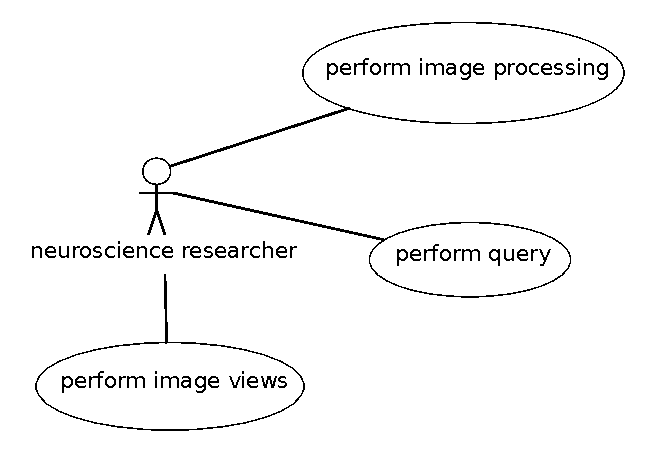
\includegraphics[width=.6\textwidth]{chapters/validation/figs/neuro-useCase.pdf}
\caption{Use Case Model~\cite{valeriaThesis}.}
\label{fig:sodm_usecase}
\end{figure}

The next model is the the extended use cases model. This model is used to model
the functionality required by the system to perform each business services.
Business services described in the previous model, become more detailed in the
extended use case model. In this model are described both the application's
features such as the possible services to be performed. Figure
\ref{fig:sodm_extendedusecase} presents the extended use case model for
\textit{perform image processing} business service. This model is detailed in 6
use cases that are necessary for the image processing. The use cases are: (i)
perform image processing; (ii) proceed with the service payment; (iii) provide
images; (iv) authenticate; (v) get results; and (vi) download results. 

\begin{figure}[ht!] 
\centering
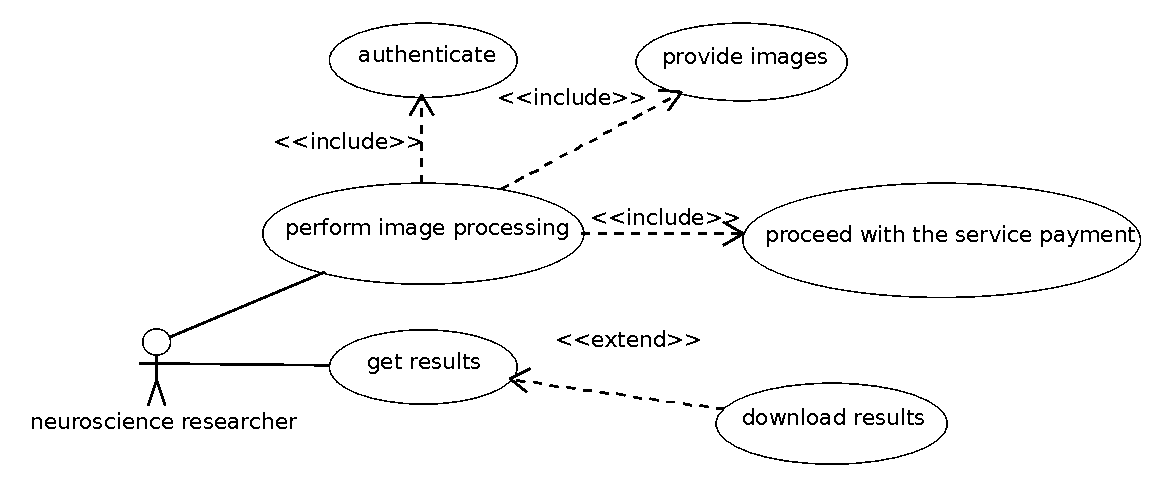
\includegraphics[width=.89\textwidth]{chapters/validation/figs/neuro-extendedUseCase.pdf}
\caption{Extended Use Case Model~\cite{valeriaThesis}.}
\label{fig:sodm_extendedusecase}
\end{figure} 
 
Once identified the different functionalities that are required by the
system to perform business services, the service process model is used to
represent the workflow necessary to perform a business service. SOD-M represents
each business service in different diagrams, which are shown in the following
figures. Figure \ref{fig:sp-imageProcessing}, for the business service ``
\textit{perform image processing}''. The activities represented in these figures
are derived from the basic use cases represented in the model extended use case.
 
\begin{figure}[ht!]
\centering
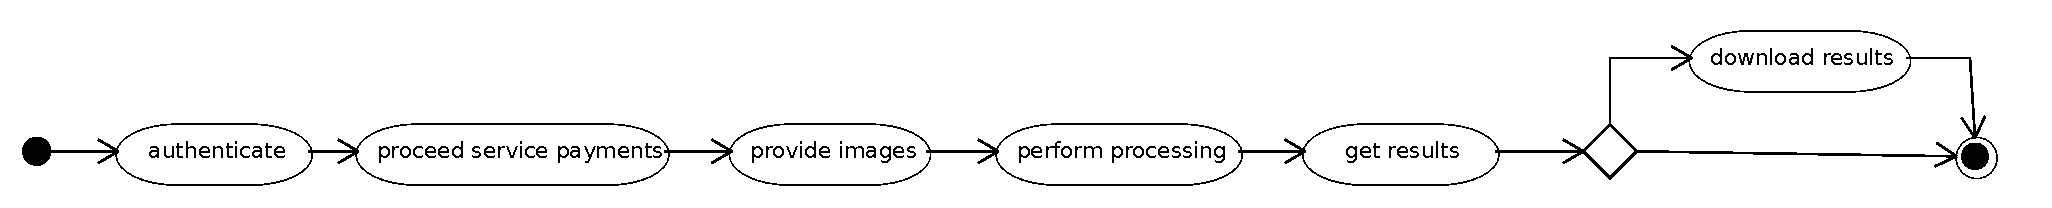
\includegraphics[width=.99\textwidth]{chapters/validation/figs/neuro-sp01.pdf}
\caption{Image Processing - Service Process Diagram~\cite{valeriaThesis}.}
\label{fig:sp-imageProcessing}
\end{figure}




% \begin{figure}[ht!]
% \centering
% 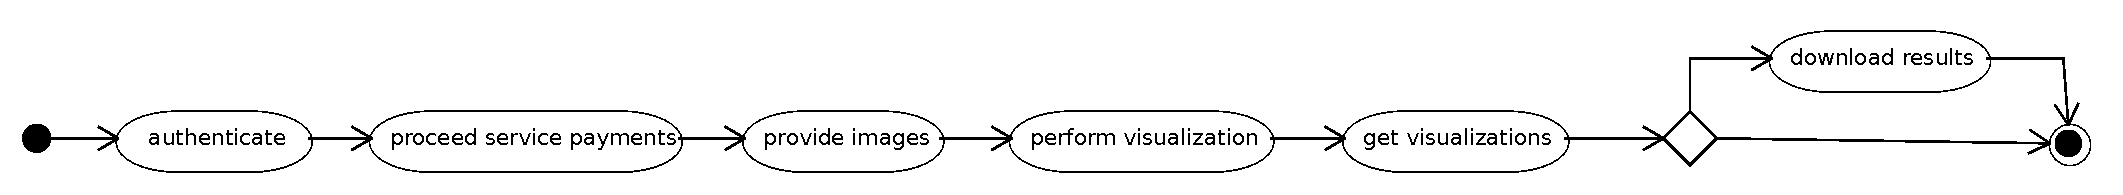
\includegraphics[width=.99\textwidth]{chapters/validation/figs/neuro-03.pdf}
% \caption{Image Visualization - Service Process Diagram~\cite{valeriaThesis}.}
% \label{fig:sp-imageVisualization}
% \end{figure}
% 
% \begin{figure}[ht!]
% \centering
% 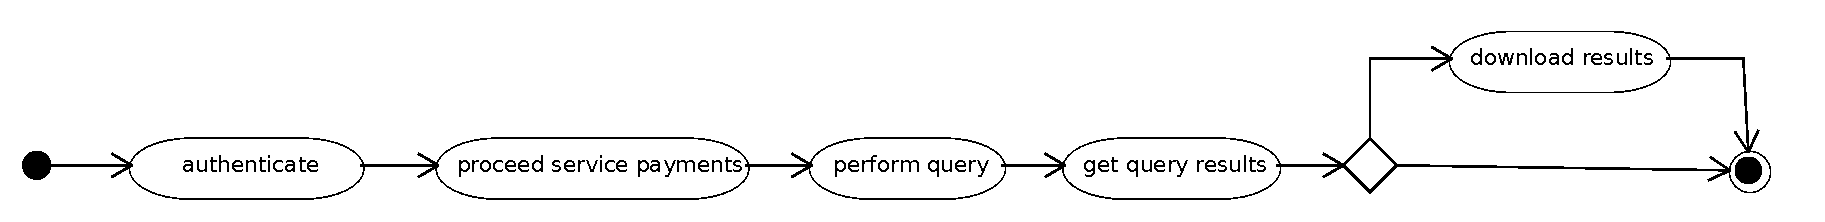
\includegraphics[width=.99\textwidth]{chapters/validation/figs/neuro-02.pdf}
% \caption{Perform Query - Service Process Diagram~\cite{valeriaThesis}.}
% \label{fig:sp-query}
% \end{figure}


The service composition models represent the processes of composition of the
various actions that are necessary to perform each business service, detailing
which business collaborator performing each action. 

 
 \begin{figure}[ht!]
\centering
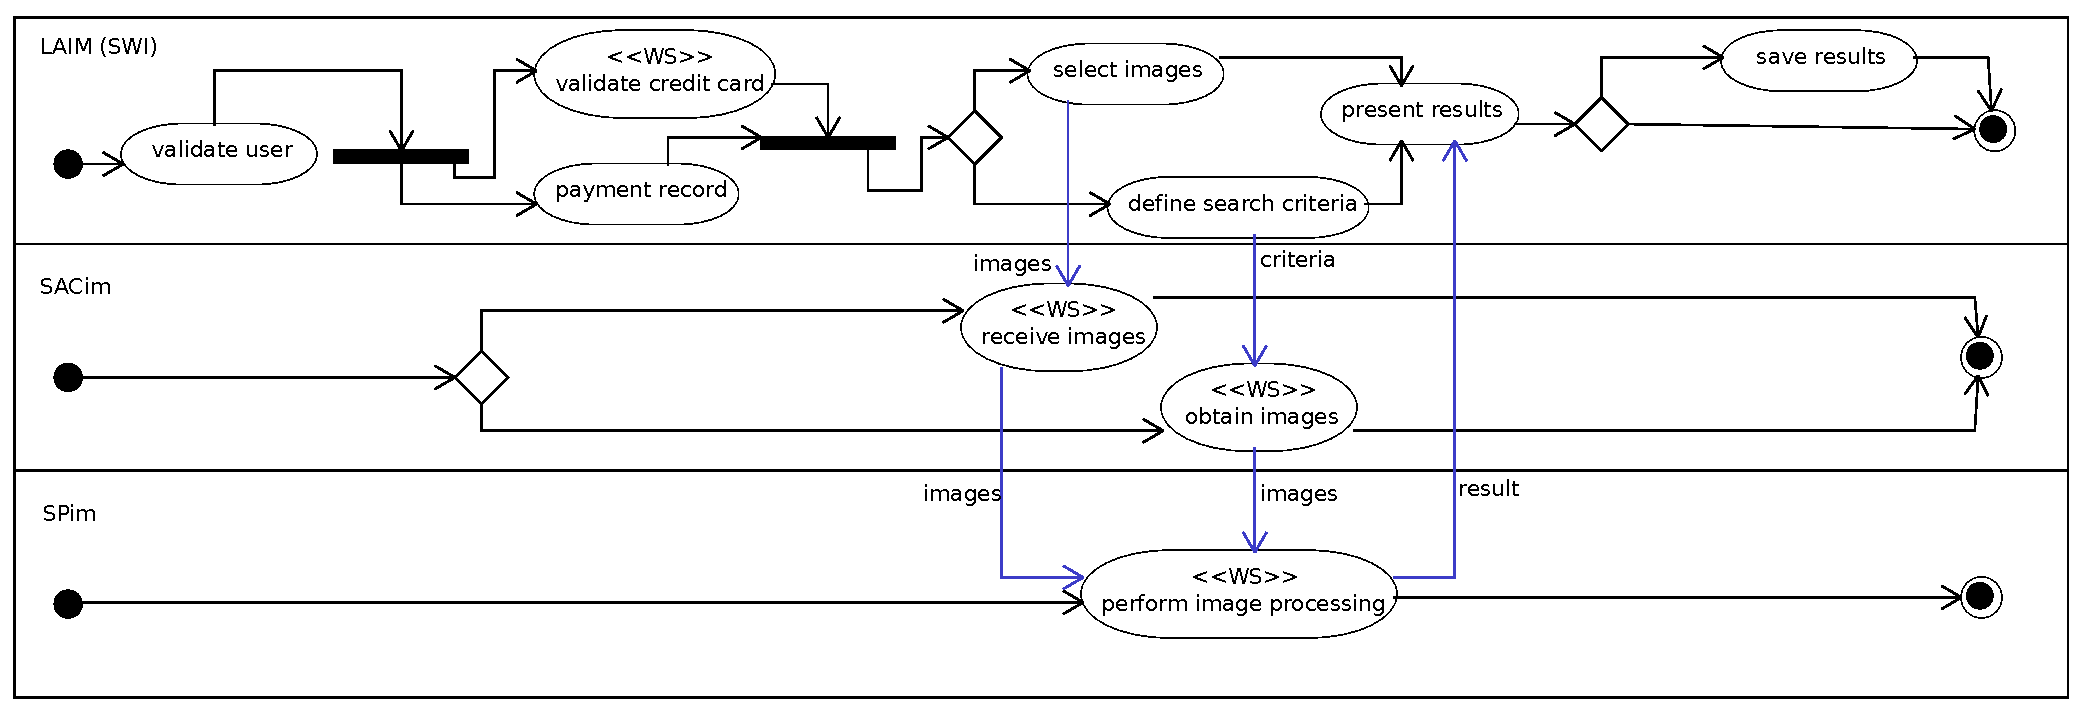
\includegraphics[width=.99\textwidth]{chapters/validation/figs/neuro-sc-01.pdf}
\caption{Image Processing - Service Composition Diagram~\cite{valeriaThesis}.}
\label{fig:sc-imageProcessing}
\end{figure}

% \begin{figure}[ht!]
% \centering
% 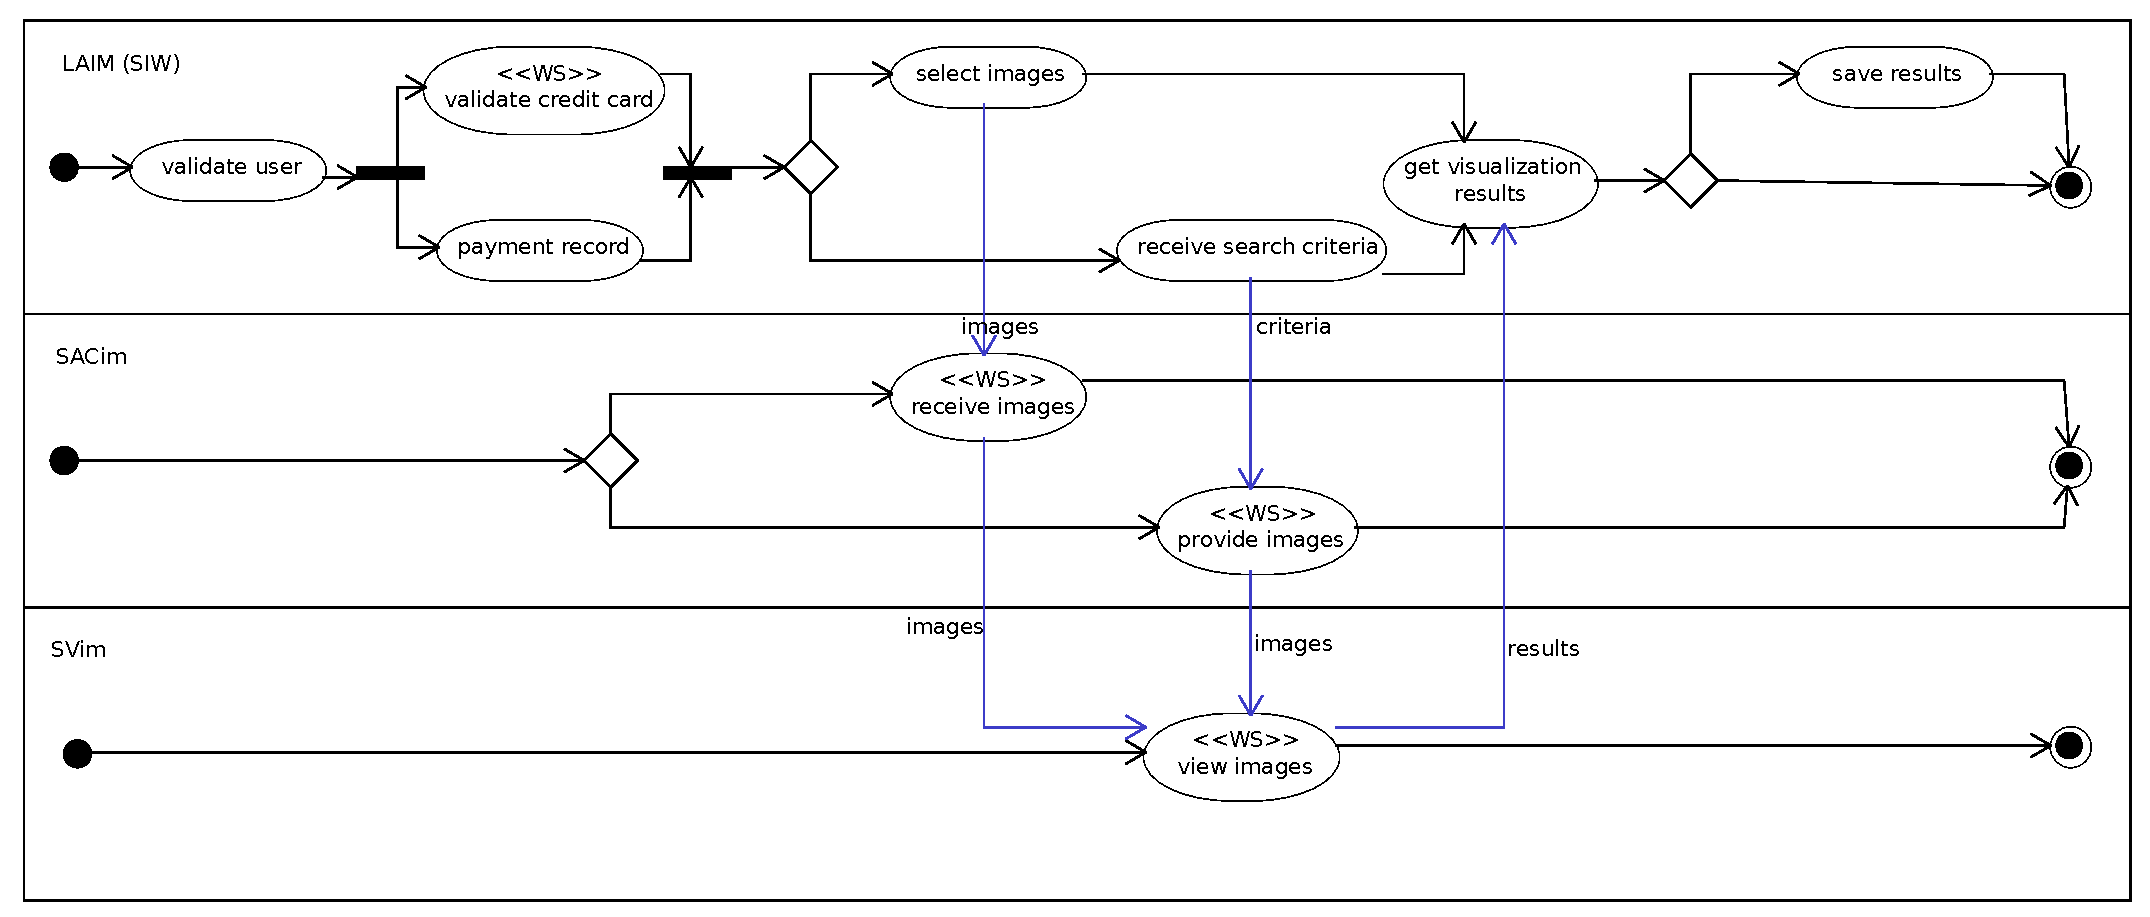
\includegraphics[width=.99\textwidth]{chapters/validation/figs/neuro-sc-02.pdf}
% \caption{Image Visualization - Service Composition
% Diagram~\cite{valeriaThesis}.}
% \label{fig:sc_example02}
% \end{figure}
% 
% \begin{figure}[ht!]
% \centering
% 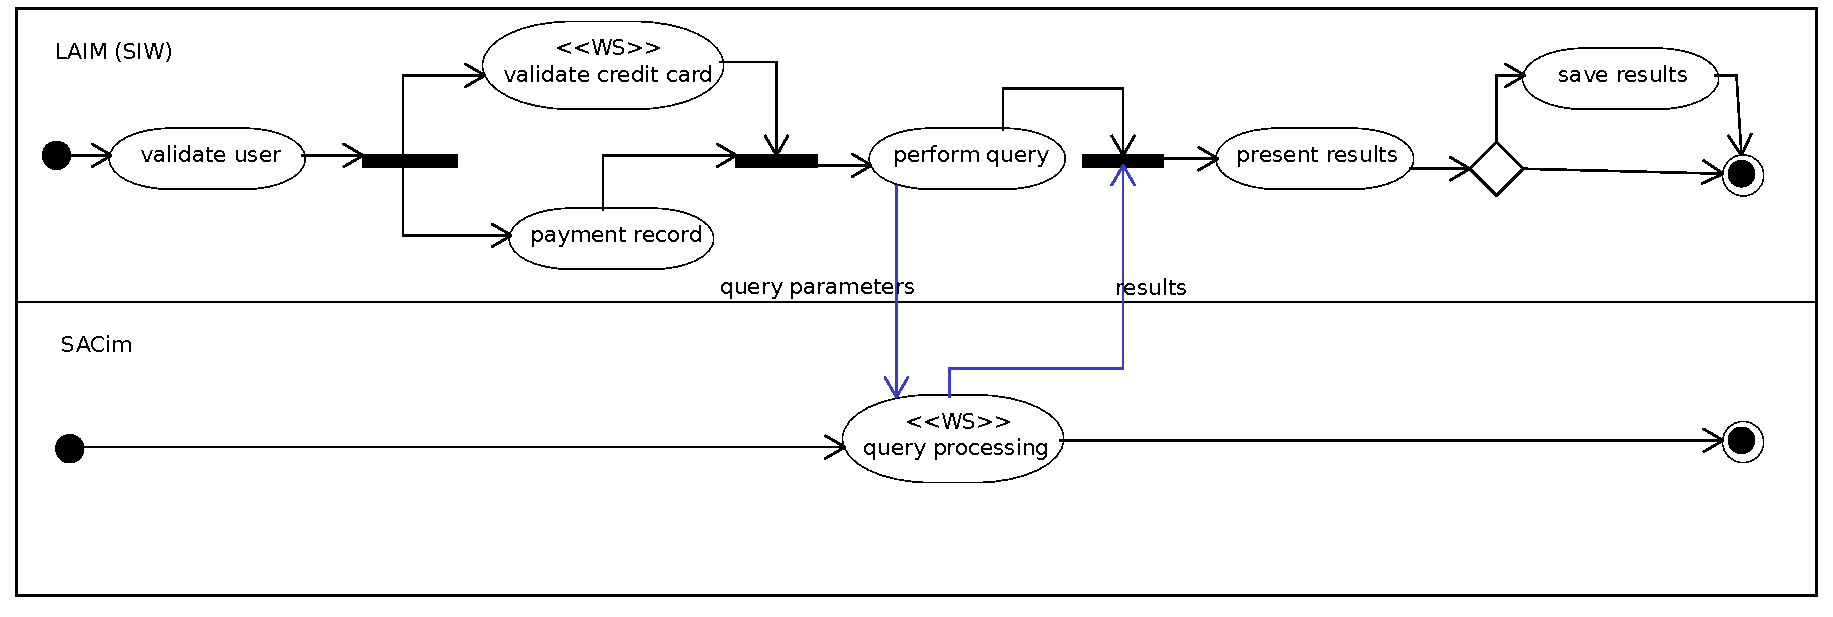
\includegraphics[width=.99\textwidth]{chapters/validation/figs/neuro-sc-03.pdf}
% \caption{Perform Query - Service Composition Diagra~\cite{valeriaThesis}.}
% \label{fig:sc_example03}  
% \end{figure} 

Figure \ref{fig:sc-imageProcessing} present the details of the services composition
for the business service we are modelling. It is important to realize that the
service processes described previously, are refined by the execution of these service.
Notice that SOD-M creates a workflow for each business service, independently.
This workflow is a sequence of services that can be run
considering the system features. Figure
\ref{fig:sc-imageProcessing} presents that the workflow
uses the services offered by LAIM to perform each function, according the SACim, SPim and SVim
services. It is also important to note that the external
application services are marked with the stereotype \textit{<<WS>>}.

The result of applying the SOD-M method is a detailed service composition model
from the business use case, in our specific case the ``\textit{perform image
processing}'' business service. 
 
 %\bigskip
 
% Notice that the non-functional properties is not modelled by SOD-M, in contract
% to $\pi$SOD-M models.



\section{Measurement and Evaluation of the $\pi$SOD-M Methodology}

Based on \cite{basili:1985}, the measurement and evaluation process requires a
mechanism for determining what data is to be collected; why it is to be
collected; and how the collected data is to be interpreted. The purpose of the measurement and
evaluation flows from the needs of the organization; the need to better
understand resource utilization in order to improve cost estimation; or the need
to evaluate the benefits, advantages and drawbacks of a research project.

The data collection process itself requires a basic paradigm that traces the
goals of the collected process, \textit{i.e.} the reasons the data are being
collected. \cite{basili:1985,Kontio:1996} describe that the need for information
must be quantified whenever possible and the quantification analyzed as to whether or not it
satisfies the needs. This quantification of the goals should then be mapped into
a set of data that can be collected.

Each evaluation \textit{goal} generates a set of questions that attempt to
define and quantify the specific goal which is at the root of its goal tree. The
\textit{goal} is only as well defined as the \textit{question} that it
generates. Each \textit{question} generates a set of \textit{metrics} or
\textit{distributions of data}.

The paradigm proposed by \cite{basili:1985} defines a set of six steps to the
data collection:

\begin{enumerate}
  \item Generate a set of goals;
  \item Derive a set of questions of interest or hypotheses which quantify those
  goals;
  \item Develop a set of data metrics and distributions which provide the
  information needed to answer the question of interest;
  \item Define a mechanism for collecting the data;
  \item Perform a evaluation of the data; 
  \item Analyze the data collected to answer the question posed.
\end{enumerate} 

\bigskip

Aiming to collect data that help in an initial analysis of our methodology
through three examples described in this chapter, we will use the approach
proposed by Basili \cite{basili:1985} to extract these data and analyze if the goals of
our proposal have been achieved and how it is possible improve the $\pi$SOD-M
methodology. 
% 
% Com o objetivo de coletar dados que auxiliem em uma análise inicial da
% metodologia proposta através dos 3 exemplos descritos neste capítulo, iremos
% utilizar a abordagem proposta por Basili para extrair esses dados e analisar se
% os objetivos da nossa proposta foram alcançados e de que forma é possível
% melhorar a metodologia $\pi$SOD-M.

\paragraph{Generate a set of goals:} First we present the goals we have, when we
intend to measurement and evaluate the $\pi$SOD-M methodology. The goals are:

% Primeiramente apresentamos os objetivos que almejamos ao realizar essa medição e
% avaliação da metodologia. Os objetivos são.
% 
% Objetivos:

\begin{enumerate}
  \item  Verify if the identification of non-functional requirements at initial
  levels of development improves the modeling of reliable web services.
  
%   Verificar se a identificação de requisitos não-funcionais nos níveis iniciais de desenvolvimento melhora a modelagem de serviços web confiáveis.

  \item  Verify how to refine application constraints into specification code,
  and if it improves the software quality.
  
%   Verificar se é possível refinar restrições de qualidade em código de especificação.

  \item  Verify if it is possible to reuse code generated for requirements
non-functional.

% Verificar se é possível a reutilização de código gerado para requisitos
% não-funcionais.

  \item  Verify how the non-functional requirements are specified in the
  methodology.

\end{enumerate}


\paragraph{Set of questions of interest which quantify the goals:} Following the
approach proposed in Basili \cite{basili:1985}, the questions are related to each goal. Table \ref{tab7:questions} present the questions related to the goals of the $\pi$SOD-M evaluation analysis.

\begin{table}
\centering
\caption{$\pi$SOD-M's Goals and Questions}
\label{tab7:questions}

\begin{tabular}{|l|l|}

\hline 
\hline \textbf{Goals} & \textbf{Questions} \\

\hline 1. Verify if the identification of non-functional & 1. What are the
levels of modeling  \\ 

requirements  at initial levels of development   & presented in the
methodology?  \\

 improves the modeling of reliable web services. &    And how the NFRs are
 modelled?  \\
 
 &  \\
 
 &  2. What is the goal of each modeling level?\\

&  \\
 
 &  3. Which kind of artifact is generated at\\
 & each level of development?\\
\hline
2. Verify how to refine application constraints & 1. What kind of modelling
approach\\

 into specification code, and if it improves &  is used in the methodology? \\
 
the software quality. & \\

& 2. How are modeled the non-functional\\
& requirements?\\

\hline

3. Verify if it is possible to reuse code  &1. Which level of development the code \\
generated for requirements non-functional. &  is generated?  and what kind of\\ 
 &code is generated?\\
&\\
& 3. The code is generated automatically \\
& or manual?\\

\hline

4. Verify how the non-functional requirements & 1. How are classified the
non-functional \\ 
are specified in the  methodology. & requirements?  \\

\hline
\hline

\hline


\end{tabular}

\end{table}
% 
% Seguindo a abordagem proposta em Basile, as perguntas referentes a cada objetivo
% são.

% OBJ1 - QUESTIONS
% 1 - Quais os níveis de modelagem que a metodologia piSOD-M apresenta? E de que
% forma os NFR são representados?
% 2 - Qual o objetivo de cada nível de modelagem
% da metodologia piSOD-M? 
% 3 - Que tipo de artefato é gerado em cada nível de desenvolvimento?
% 
% OBJ2 - QUESTIONS
% 1 - Qual abordagem de desenvolvimento é utilizada na metodologia?
% 2 - Como são modelados os requisitos não-funcionais?
% 
% OBJ3 - QUESTIONS
% 1 - Em qual nível de desenvolvimento o código é gerado? E que tipo de código é
% gerado? 
% 2 - O código é gerado de maneira automática ou manual?
% 
% OBJ4 - QUESTIONS
% 1 - Como são classificados os requisitos não-funcionais?
% 2 - Existe algum tipo de classificação dos RNF?


% Ainda seguindo a abordagem proposta por Basili, identificamos métricas com o
% objetivo de quantificar as perguntas, de forma a gerar dados que possam ser
% analisado e avaliados com o objetivo de verificar se os objetivos da avaliação
% foi satisfeito. As métricas são por listadas por objetivos/questões (por
% exemplo, #1.2. Esta métrica está relacionada ao objetivo 1, e a questão 2
% identificados anteriormente), dessa forma as medidas a serem quantificadas são
% apresentadas na tabela X.

\paragraph{Set of data metrics and distributions:} Still following the approach
proposed by Basili \cite{basili:1985}, we identify metrics with the objective of quantify the questions in order to generate data that can be
analyzed and evaluated in order to verify that the goals of the evaluation
were satisfied, or not. The metrics are listed by goal/question (for
example \#1.2. This metric is related to \textit{goal} 1, and \textit{question}
2 previously identified). The statements for measure the data are
shown in table \ref{tab8:metrics}.

\begin{table}
\centering
\caption{$\pi$SOD-M's Metrics/Distributions}
\label{tab8:metrics}

\begin{tabular}{|c|l|}

\hline 
\hline \textbf{Goal/Question} & \textbf{Metrics/Distributions} \\

\hline \#1.1 & 1. How many levels the methodology defines?  \\
& 2. How many models are generated at each level?\\
\hline \#1.2 & 1. How many restrictions were modeled (by level)?  \\
\hline \#1.3 & 1. How many artifacts were generated (by level)?  \\
\hline \#2.1 & 1. How long (in days) was spent for the modeling   \\
&  of each case study? \\
\hline \#2.2 & 1. How many RNFs were modeled using the approach?  \\
\hline \#3.1 & 1. How many lines of code were generated for \\
& specify the non-functional requirement identified? \\

\hline \#3.2 & 1. What is the total of line of code generated? \\

\hline \#4.1 &  1. How many types of non-functional requirements \\
& were identified?\\

 &  2. Which non-functional requirements \\
& were identified?\\

\hline
\hline

\hline


\end{tabular}

\end{table}

% Metricas
% 
% 1.1.1 Quantos níveis a metodologia define?
% 1.1.2 Quantos modelos são gerados em cada nível?
% 
% 1.2.1 Quantas restrições são modelada?
% 
% 1.3.1 Quantos artefatos podem ser gerados?
% 
% 2.1.1 Qual o tempo médio para o desenvolvimento de cada estudo de caso?
% 2.2.1 Quantos RNF foram modelados?
% 
% 3.1.1 Quantas línhas de código foram geradas para cada requisito não funcional
% identificado?
% 3.2.1 Qual a soma total de linha de código geradas?
% 
% 4.1.1 e 4.1.2 Quantos tipos de requisitos não-funcionais foram identificados?
%  

\paragraph{Collecting the data:} After the development of metrics and the types
of data to be collected, the extraction was performed considering the modeling
steps of $\pi$SOD-M for each case study presented in this chapter. Table
\ref{tab9:data} presents the results of the data collection.   

  
\paragraph{Evaluation of the data:} Tables \ref{tab8:metrics} and
\ref{tab9:data} present the questions and data generated from the evaluation of
each example. All examples were modeled in accordance with the proposed
methodology and yielded the following results.

% As tabelas 9 e 10 apresentam as perguntas e os dados gerados a partir da
% avaliação de cada exemplo. Todos os exemplos foram modelados de acordo com a
% metodologia e gerou os seguintes resultados.

\begin{table} 
\centering
\caption{Results: $\pi$SOD-M's Metrics/Distributions}
\label{tab9:data}

\begin{tabular}{|c|c|c|c|}
\hline 
\cline{2-4}
& \multicolumn{3}{ |c| }{$\pi$SOD-M} \\
\hline  
Metrics/Distributions & Example 1 & Example 2 & Example 3 
\\
\hline 
\hline \#1.1.1 & 4 & 4 & 4 \\
\hline \#1.1.2 & 1-1-1-1 & 2-2-2-2 & 3-1-1-1 \\
\hline \#1.2.1 & 5c-8a-6r-2co & 7c-9a-7r-5co & 4c-6a-6r-3co\\
\hline \#1.3.1 & 1 & 1 & 1 \\
\hline \#2.1.1 & 8 & 10 & 5\\
\hline \#2.2.1 & 2& 3& 3\\
\hline \#3.1.1 &9 & 37 & 20 \\
\hline \#3.2.1 & 29 & 56& 40\\
\hline \#4.1.1 & 2& 3& 3\\
%\hline \#4.1.2 & & & \\

\hline

\end{tabular}
\end{table}


The methodology defines 4 levels of modeling (\textit{\#1.1.1}), however the
case studies generated a different number of models ($\pi$-UseCase,
$\pi$-ServiceProcess, $\pi$-ServiceComposition e $\pi$-PEWS). In \textit{Example
1} was generated 1 model of each type, in \textit{Example 2} were generated two
models of each type, and in \textit{Example 3} were generated 3 $\pi$-UseCase
models and 1 referring to the others (\textit{\#1.1.2}). We found that this
variation has no involvement with the identification of the number of non-functional
requirements.

% A metodologia define 4 níveis de modelagem, no entanto os estudos de caso
% geraram um número diferente na quantidade de modelos ($\pi$-UseCase,
% $\pi$-ServiceProcess, $\pi$-ServiceComposition e $\pi$-PEWS). No exemplo 1 foram
% gerados 1 modelo de cada, No exemplo 2 foram gerados 2 modelos de cada tipo, e
% por fim, o exemplo 3 gerou 3 modelo de caso de uso e 1 referente aos demais.
% verificamos que essa variação não tem nenhuma implicação com a identificação dos
% requisitos.

Regarding the types of restrictions modeled at each level, we find that
the number constraints identified implies an increase in the number of
lines of code. The  \textit{Example 1} set five \textit{constraints} in the
$\pi$-UseCase model, 8 \textit{assertions} in the $\pi$-ServiceProcess model, 6
\textit{rules} in the $\pi$-ServiceComposition model and 2 \textit{contracts} in
the $\pi$-PEWS model (\textit{5c-8a-6r-2Co} \footnote{5c =
5 constraints, assertions 8th = 8; 6r = 6 rules; 2Co contracts = 2}). This
example generated 29 lines of code specification. However, the \textit{Example
2} presents the following data \textit{7c-9a-7r-5co}, generating 56 lines of
specification code. It was observed that the number of restriction increases the
number of lines specification. The \textit{Example 3} presents the following
data, \textit{4c-6a-6r-3co}, generating 40 code lines specification
(\textit{\#1.2.1}, \textit{\#3.1.1} and \textit{\#3.2.1}).


% Em relação aos tipos de resquições modeladas em cada nível, verificamos que
% quanto mais restrições são identificadas implica em um aumento no número de
% lineas de código. O exemplo defini 5 constraints no modelo de $\pi$-UseCase, 8
% assertions no modelo de $\pi$-ServiceProcess, 6 regras no modelo de
% $\pi$-ServiceComposition e 2 contratos no modelo de $\pi$-PEWS
% (\textit{5c-8a-6r-2co}\footnote{5c = 5 constraints; 8a = 8 assertions; 6r = 6
% regras; 2co = 2 contratos}). Esse exemplo tem 29 linhas de código de
% especificação. Enquanto o exemplo 2 apresenta o seguinte dado, 7c-9a-7r-5co,
% gerando 56 linhas de código de especificação. Percebe-se que o número de
% restrições aumenta o número de linhas de especificação. O exemplo 3 tem as
% seguintes resquições, 4c-6a-6r-3co, gerando 40 linhas de código de
% especificação.

According to the data analysis, we also found that the number of lines of code
for the definition of contracts increase according to the numbers of rules
identified (\textit{\#1.2.1}). 

The number of days spent for modeling also varied
according to the number of constraints. Thus, the time spent with
identification and modeling of the constraints implies a greater number of days
of development. \textit{Example 2} was modeled in 10 days (\textit{\#2.1.1}) and
this example showed a greater number of restrictions and non-functional
requirements. We assume that if these restrictions were not modeled since the initial stages, the time spent on
maintenance could be higher. \textit{Example 3} had the fewest
number of restrictions, and therefore took less time to be modeled. Thus the
number of non-functional requirements of an application implies the time spent
for the project development using $\pi$SOD-M (\textit{\#2.2.1} and
\textit{\#4.1.1}).

% Segundo a análise, verificamos também que o número de linha de especificação em
% apenas para a definiçào dos contratos, cresce de acordo com o números de regras
% identificadas. A quantidade de dias gastos para a modelagem também variou de
% acordo com o número de restrições da aplicação. Dessa forma, o tempo gasto com a
% identificação e modelagem das restrições do exemplo teve uma implicação direta
% com o número de dias gastos. O exemplo 2 foi modelago em 10 dias e este
% apresentou um número maior de restrições, e requisitos não funcionais. Podemos
% supor que se essas restrições não fossem modeladas desde as etapas iniciais, o
% tempo gasto com manutenção poderia ser maior. O exemplo 3 teve o menor número de
% restrições, e consequentemente levou menos tempo para ser modelado. Dessa forma
% o número de requisitos não-funcionais de uma aplicação implica no tempo gasto
% no desenvolvimento do projeto.

\paragraph{Conclusions:}

We conclude that the identification of NFRs in initial levels of modelling helps
the development of services, mainly because the restrictions can be
refined and transformed into code specification. This favors the
prior identification of errors, and help in the classification of the
non-functional requirements.

Classify restrictions as constraints, then refine this concept into assertions,
and then group it into policy improves identifying types of non-functional
requirements, providing reusability of services and better use of the code
specification.

We also found that the use of the method provides identification of different
types of NFRs. These requirements are translated into contracts and can be
checked at runtime. We can see that the number of lines of code generated
for each type of non-functional requirement does not have a regular variation,
and it does not generates apparent side effects.



\subsection{Comparison of the SOD-M and $\pi$SOD-M approaches}

% A tabela X apresenta dados em relacao aos 3 exemplos utilizados na avaliacao. O
% resultado reflete as diferencaos entre as duas abordagem com a intencao de
% verificar como a extensao de SOD-M pode melhorar o processo de modelagem de
% aplicacoes orientadas a servicos na presenta de requisitos nao funcionais. 
\newText{
We also perform a comparative analysis between $\pi$SOD-M and SOD-M,
considering other aspects. Table \ref{tab6:comparison} presents the data related with the
three examples used for the $\pi$SOD-M evaluation: (i) To Publish Music example (\textit{Ex. 1}),  (ii) Crime Map example (\textit{Ex. 2}), and  (iii) GesIMED
example (\textit{Ex. 3}). The result reflects the difference between the two
approaches (SOD-M and $\pi$SOD-M) with the intention of verifying how $\pi$SOD-M
can improve the modeling process of service-oriented applications in the presence of
non-functional requirements. }
 

% Os aspectos analisados foram: (i) a quantidade de use cases necessarios para a
% modelagem de mais alto nivel tanto dos requisitos como das restricoes da
% aplicacao; (ii) quantas actions sao necessarias para a representacao do processo
% de negocio; (iii) quando business collaborators sao necessarios para a
% execucao completa do workflow; (iv) quantos requisitos nao funcionais foram
% identificados durante a modelagem da aplicacao; (v) quantas linhas de codigo
% podem ser geradas a partir do modelo de composicao de servicos; e (vi) quantas
% transformacoes de modelos sao realizadas durante todo o processo de
% desenvolvimento.
\newText{
The aspects analyzed and presented in table \ref{tab6:comparison} are: (i) the
number of use cases required for modeling both, the
restrictions and requirements of the application, (ii) how many actions are required for the
representation of the business process, (iii) how many business collaborators
are needed to the complete execution of the workflow, (iv) the number of
non-functional requirements that were identified during the modeling of the
application, (v) how many lines of code were generated from the service
composition model of each example, and (vi) how many model transformations held
throughout the development process.
}




% Considerando o numero de casos de uso necessarios para a modelagem dos exemplos
% apresentados neste capitulo, os exemplo modelados com piSOD-M apresentam mais
% casos de uso pois e possivel modelar as restricoes da aplicacao atraves de casos
% de uso esteriotipados com o esteriotipo costraint. Devido a este motivo o
% exemplo 1 apresenta 9 casos de uso usando SOD-M, enquanto que utilizando a
% abordagem piSOD-M se tem 13 casos de uso. A diferenca (4 casos de uso)
% representa a quantidade de restricoes que foi identificada neste nivel atraves
% do modelo de pi-UseCase. No exemplo 2 temos 8 casos de uso utilizando SOD-M
% enquanto temos 13 utilizando piSOD-M. Uma diferenca de 5 casos de uso. E por fim
% o exemplo 3 temos 5 casos de uso utilizando SOD-M, e 9 casos de uso atraves da
% modelagem com piSOD-M.  piSOD-M apresenta uma quantidade maior de casos de uso
% pelo fato deste modelo tambem representar as restricoes da aplicacao, mesmo no
% nivel mais abstrado. Verificamos que apesar, de um esforco relativamente maior
% de modelagem, a representatividade do modelo no que diz respeito aos requisitos
% funcionais e nao-funcionais e maior em piSOD-M que em SOD-M.

\newText{
Considering the number of use cases for modeling the examples presented in this
chapter, the models from the $\pi$SOD-M approach present more use cases then
the models in SOD-M, because using $\pi$SOD-M it is possible to model the
restrictions of the application through stereotyped use cases
(\textit{constraint}). Due to this reason, example 1 has 9
use cases using SOD-M, while using $\pi$SOD-M, the model has 13 use cases. The difference (4 use cases) between
both approaches represents the amount of restrictions that have been identified
at this level through the $\pi$-UseCase model. In example 2, it has 8 use cases
using SOD-M while using $\pi$SOD-M it has 13 use cases. A difference of 5 use
cases. In the third example, it presents 5 use cases using SOD-M, and 9 cases
through $\pi$SOD-M. $\pi$SOD-M presents a greater number of use cases because
this model also represent the constraints of the application, even in the most
abstract level. We found that in spite of a relatively greater effort modeling,
$\pi$SOD-M describes functional and non-functional aspects, while SOD-M models
only functional aspects.
}


\begin{table}
\centering
\caption{Comparison: SOD-M and $\pi$SOD-M}
\label{tab6:comparison}

\begin{tabular}{r|c|c|c||c|c|c|}


\cline{2-7}
& \multicolumn{3}{ |c|| }{SOD-M} & \multicolumn{3}{ |c| }{$\pi$SOD-M} \\

\cline{2-7} & Ex. 1 & Ex. 2 & Ex. 3 & Ex.
1 & Ex. 2 & Ex. 3
\\
\hline 
\hline Use Case &9 &8 & 5& 13 & 14 &9\\
\hline Action &7 & 7 &5 &15 &12 &11\\
\hline Business  & 4&3 &3 &4 &3 &3\\
       Collaborator & & & & & &\\
\hline NFRs & - & - & - &2 &3 &3\\
	   modelled &  &  &  & & &\\
\hline Lines & 20 & 19 &20 & 29 & 56&40\\
	   of Code & & & & & &\\
\hline Transformations  & 2 & 2 & 2 & 3 & 3 & 3\\


\hline

\end{tabular}

\end{table}

% Em relacao ao numero de actions, a nossa abordagem apresenta um numero maior
% pois e necessário descrever pre- e pos-condições para a execuçao do workflow. O
% numero maior de actions em piSOD-M favorece que a execução do workflow obedeça a
% restrições do sistema. Estas actions são resultado das trasnformações dos casos
% de uso. Os casos de uso marcados com esteriotipos constraint, sao transformados
% em actions com esteriotipos assertion. É importante perceber na tabela, que no
% primeiro exemplo, o numero de action varia de 7 para 15, no segundo de 7 para 12
% e no terceiro exemplo varia de 5 para 11. A verificação de restrições atravéd de
% assertions favorece a representacao de requisitos nao-funcionais necessários
% para a execução do workflow.

\newText{
In relation to the number of actions, the $\pi$SOD-M approach provides a larger
number, because it needs to describe pre- and post-conditions for the
services. The larger number of actions in $\pi$SOD-M favors the verification of
restrictions during the execution of the workflow. These
actions are the result of a model transformation. The use cases marked
with \textit{constraint} stereotype are transformed into actions with
the \textit{assertion} stereotype. It is important to realize in the table that
in the first example, the number of action ranges from 7 to 15,  the second 7
to 12 and in the third example ranges from 5 to 11. The constraint checking
through assertions favors the representation of non-functional requirements
necessary for the workflow execution.
}


% Considerando o número de Business Collaborator, esse valor nao sofre nenhuma
% variação entre as abordagens, pelo fado dos serviços a serem executados nos 3
% exemplos e nas 2 abordagens serem os mesmos. Apesar do número de casos de uso e
% actions variarem isso não implica na variação da quantidade de serviços externos
% (business collaborator) necessários para a execução da aplicação.

\newText{Considering the number of \textit{Business Collaborator}, this value does not
suffer any variation between both approaches, because of the services to be
performed in the 3 examples in both approaches are the same. Although the number
of use cases and actions vary, it does not imply the variation of the amount of external
services (\textit{Business Collaborator}) required for execute the application.  
}
  

% Como o objetivo de ambas as abordagens são destintos, verificar a quantidade de
% requisitos não-funcionais não é comparável, no entanto aponta para uma melhoria
% e evolução da abordagem SOD-M. Usando SOD-M não é possível identificar nenhum
% requisito não funcional durante a modelagem. No entanto em piSOD-M é possível
% modelar distintos requisitos não-funcionais e refina-los durante a modelagem,
% fazendo com que em um nível mais baixo sejam representados como propriedades não
% funcionais \cite{MylopoulosBook99}. Apesar de não ser comparável pois ambas as
% abordagens tem focos de desenvolvimento diferentes, a proposta apresentada em
% piSOD-M abraga um valor razoável ao considerar a modelagem de requisitos não
% funcionais para aplicaçoes orientadas a serviços.

\newText{
Since the goal of SOD-M and $\pi$SOD-M approaches are different, analyze the number of
non-functional requirements modelled is not
comparable, however points to an evolution and improvement of the SOD-M approach. Using SOD-M, it is not possible
to identify any non-functional requirement during the modeling. However, using
$\pi$SOD-M, it is possible to model different non-functional requirements and
refine them. From this point of view, both approaches are not comparable because
they have different focus of development, otherwise the proposal presented in
$\pi$SOD-M adds reasonable value considering the modeling of non-functional
requirements for service-oriented applications.
}

% Considerando a especificação das aplicações descritas em cada na lingagem
% piPEWS, fazemos uma análise da diferença do número de linhas geradas em relação
% as ambas abordagens. Como a modelagem em SOD-M considera apenas a especificação
% dos requisitos funcionais, e piSOD-M consideram ambos aspectos, funcionais e não
% funcionais, a análise compara a especificação piPEWS de cada exemplo,
% considerando a geração dos contratos (piSOD-M) e a não geração dos contratos
% (SOD-M) que representam a verificação de aspectios não-funcionais. O número de
% linha e código cresce em piSOD-M devido ao fato da espeficicação gerar contratos
% que definem pre e pos-condições sobre os serviços do workflow. O crescimento
% depende da quantidade de restrições descritas durante a modelagem dos exemplos.
% Não existe nenhum padrão com relação a diferença de número de linhas de código.
% Por exemplo,o exemplo 1 a diferença entre as abordagens é de 9 linhas de código,
% enquanto o exemplo 2 a diferença é de 37 linhas. No exemplo 3 a diferença é de
% 20 linhas de código, sendo 20 linhas geradas usando a abordagem SOD-M e 40
% usando a abordagem piSOD-M. É importante notar que o número de requisitos não
% funcionais modelados tem como consequencia um maior número de linhas de código,
% perceba-se os exemplos 2 e 3, pois ambos modelam 3 requisitos não-funcionais e
% isso implica em um número maior de linhas de na especificação em piPEWS.

\newText{
Regarding the specification code for each example, we analyzed the difference of
lines of code ($\pi$-PEWS language) generated in both approaches. SOD-M
only considers the specification of functional aspects, and $\pi$SOD-M consider both aspects, functional and non-functional,
thereby we compare the $\pi$-PEWS specification for each example, considering the
generation of the workflow (SOD-M)  and the generation of contracts
($\pi$SOD-M). The number of lines of specification grows in $\pi$SOD-M due to
the fact that this approach generates contracts which defines pre- and post-conditions
for the services. The growth depends on the number of constraints identified
during the modeling. There is no standard concerning the difference in terms of the number of lines
generated. For example, in the first example the difference between the
approaches is 9 lines of code, while in the second example the difference is 37
lines. In the example 3 the difference is 20 lines of code, where 20 lines were
generated using the SOD-M approach  and 40 lines using $\pi$SOD-M. We can
conclude is that the number of non-functional requirements modeled implies a greater number of lines of specification code, to realize the examples
2 and 3, both has three non-functional requirements and it implied a larger
number of lines in $\pi$-PEWS specification, 56 e 40 respectively.
}



% Outro fator a ser analisado é o número de transformações em cada abordagem. Na
% modelagem de todos os exemplos em SOD-M foram realisadas 2 transformações no
% nível PIM, enquanto que na modelagem dos exemplos usando piSOD-M foram
% realizadas 3 trasnformações, 2 no nível PIM e 1 no nível PSM. O número maior de
% transformações implica em um maior refinamento dos conceitos, e consequentemente
% na geração de código para uma plataforma específica.

\newText{
Another factor to be considered is the number of transformations in each
approach. In the modeling of all the examples in SOD-M were performed two 
transformations at PIM level, whereas in the modeling of the examples using
$\pi$SOD-M were performed three transformation, 2 in the PIM level and 1 on PSM
level. The larger number of transformations in $\pi$SOD-M represents a step of
refinement and the generation of code for a specific platform.      
}

% 
% Apesar dos números apresentados na tabela X mostrarem que existe um esforço
% maior no uso da metodologia piSOD-M, isso se deve ao fato de que restrições
% sobre requisitos e serviços saão feitas desde os níveis mais abstratos de
% modelagem. Isso favorece a identificação prévia e revinamento adequado de
% aspectos transversais e restrições da aplicação. A metodologia piSOD-M agrega
% valor e conceitos novos em relação a SOD-M melhorando e facilitando a descrição
% de requisitos de qualidade das aplicações orientadas a serviços.

\newText{
Despite the numbers presented in table \ref{tab6:comparison} show that there is a
larger effort in the use of the $\pi$SOD-M methodology, compared with SOD-M,
this is due to the fact that non-functional requirements and restrictions on
services are made from the most abstract levels of modeling. This favors the
early identification of system restrictions and improves the refinement of
transversal aspects and constraints of the application. The 
$\pi$SOD-M methodology adds reasonable value and new concepts regarding SOD-M,
improving and facilitating the description of quality requirements for
service-oriented applications. }  

\section{Conclusions}
\label{sec:conclusion_validation}

This chapter presented the use of the $\pi$SOD-M methodology, as a form of
empirical validation. We described, modeled and implemented three
\correctingText{example of application development} to use concepts, model
properties and detail the process development. The methodology and its concepts supported the development of applications that use service
compositions, mainly in the identification and refinement of quality requirements. The use of $\pi$SOD-M
and its environment can help to identify the non-functional requirements and
improve the system modeling and specification process.
  
We conducted, in this chapter, two types of evaluations, the first followed the
proposal based on Basili~\cite{basili:1985} for data evaluation. And the second
was a comparison between $\pi$SOD-M and SOD-M, considering different aspects. 
  
\newText{The development of applications by using SOD-M favors and improves
the modelling of services in more abstract levels of development and help to
identify non-functional requirements related with each of these services.}

The transformations of models enables the semi-automatic
development of applications. Owing to the generation of the
system specification code from the service composition model, the designer and
developer can focus on the description and detail of functional and non-functional requirements. The
generated code contains the expression of the interaction with services and
their associated namespaces. This specification can be executed after the model
transformation.

As the process is iterative and incremental, after the generation of each model
it is possible to make adjustments to the generated model. For example, after
the $\pi$-UseCase model design and the generation of $\pi$-ServiceProcess 
model, the designer can make adjustments and improve the model so that it
becomes more expressive. 

 

